% Statistics creative and short question bank: First Paper + Second Paper.
% This is the single source file. Compile from question/ (twice, for the contents page):
%   pdflatex stat_cq_bank.tex
\documentclass[a4paper,oneside]{book}
\usepackage{float}
\usepackage{amsmath}
\usepackage{xcolor}
\usepackage[hidelinks]{hyperref}
\usepackage[a4paper, total={7.27in, 10.69in}]{geometry}
\usepackage{titletoc}
\usepackage{graphicx}
\usepackage{tikz} % for drawing labeled lines
\usetikzlibrary{calc} % for drawing labeled lines

\titlecontents*{chapter}
  [0pt]% <left>
  {}
  {\chaptername\ \thecontentslabel\quad}
  {}
  {\bfseries\hfill\contentspage}

\usepackage{bookmark}
\usepackage{etoolbox}

\makeatletter
\newcommand*{\AddChapterPrefixInBookmarks}{%
  \if@mainmatter
    \ifnum\bookmarkget{level}=0 %
      \preto\bookmark@text{\@chapapp\space}%
    \fi
  \fi
}
\makeatother

\bookmarksetup{
  numbered,
  addtohook=\AddChapterPrefixInBookmarks,
}

% Workaround for numbered sections in unnumbered
% chapter "Introduction" to avoid chapter number
% zero.
\renewcommand*{\thesection}{%
  \ifcase\value{chapter}%
  \else
    \thechapter.%
  \fi
  \arabic{section}%
}

\pagestyle{headings}

\DeclareUnicodeCharacter{20B9}{Rs.}% the rupee sign
\providecommand{\fillin}[1]{\textcolor{red}{#1}}% review notes (\fillin is from the exam class)

\begin{document}
\frontmatter

\begin{titlepage}
    \begin{center}
        \vspace*{1cm}
        \Huge
        \textbf{Statistics Question Bank}

        \vspace{0.5cm}
        \LARGE
        First and Second Paper

        \vspace{1.5cm}
        \textbf{Abdullah Al Mahmud}

        \vspace{1.5cm}
        \Large
        Updated on: \today

        \vfill
        
\includegraphics[width=1cm]{img/logo2.0.png}

        \Large
        www.statmania.info\\
    \end{center}
\end{titlepage}

\tableofcontents

\mainmatter

% ============================== PAPER 1 ==============================
\renewcommand{\theHchapter}{1.\arabic{chapter}}% unique link names per paper
\part{First Paper}

\chapter{Statistics, Variable and Concepts of Different Symbols} 

\section{Creative Questions}

\begin{enumerate}

     \item
	  \textbf{A system analyst collected frequencies of a signal at different times. Then he realized due to some unknown noise, 0.5 units got added to all the values. The recorded values are given below:} 
	  
	  \begin{center}
	  10, 12, 15, 14, 12, 16, 20, 16, 18, 11
	  \end{center}
  
  \begin{enumerate}
    \item
	What is change of origin? \hfill 1
    \item
	Does change of origin have an effect on median? \hfill 2
    \item  
	Find $\displaystyle \sum_{i=1}^{10} (X_i-5)$. \hfill 3
    \item
	Determine the summation of the values discarding the noise. \hfill 4
  \end{enumerate}
  
  \item  
\textbf{The daily website visits (in thousands) for an online platform over seven days are recorded as 80, 85, 90, 95, 100, 105, and 110 (denoted by \textit{z}). The platform analyst claimed that the square of the total visits is greater than the total of the squared visits.}

\begin{enumerate}
    \item  
    Calculate $\displaystyle \sum_{i=1}^7 (z_i - 2z_i)^2$ using the provided data. \hfill 3
    \item
    Verify whether the analyst’s statement is accurate based on the data. \hfill 4
\end{enumerate}

\item
\textbf{The weekly sales (in hundreds of dollars) for a retail store over six weeks are recorded as 12, 15, 18, 20, 22, and 25 (denoted by \( y \)). The store manager claimed that the square of total sales exceeds the total of squared sales.}

\begin{enumerate}
    \item
    Calculate $\displaystyle \sum_{i=1}^6 (y_i - 3y_i)^2$ using the provided data. \hfill 3
    
    \item
    Determine whether the manager’s claim is correct based on the data. \hfill 4
\end{enumerate}
  
  \item
\textbf{A software developer tracked the response times (in milliseconds) 
of a web application under test during peak usage hours. An unexpected 
delay of 1.2 ms was added to each recorded response time due to server
lag. The recorded times are as follows:}

\begin{center}
45, 48, 52, 50, 47, 53, 60, 55, 58, 49
\end{center}

\begin{enumerate}
    \item  
    Calculate $\displaystyle \sum_{i=1}^{10} (X_i - 25)$. \hfill 3
    \item
    Find the sum of the original response times before the lag was added. \hfill 4
\end{enumerate}

  
  \item
\textbf{The monthly sales (in thousands of units) recorded by a store over 
five months are 120, 135, 150, 160, and 175. The store manager 
stated that the square of the total sales is greater than the total of 
the squared sales.}

\begin{enumerate}
    \item  
    Calculate $\displaystyle \sum_{i=1}^5 (x_i - 1.5x_i)^2$ using the 
    provided data. \hfill 3
    \item
    Assess whether the manager’s statement is accurate based on the data. \hfill 4
\end{enumerate}

  \item  
  \textbf{A nutritionist is analyzing the daily protein intake (in grams) of five athletes.  
  The recorded values are:}  
  \begin{center}
  $x_1 = 55,\quad x_2 = 60,\quad x_3 = 48,\quad x_4 = 62,\quad x_5 = 50$
  \end{center}

  \begin{enumerate}
    \item  
    Compute the value of $\displaystyle \sum_{i=1}^5 (x_i - 52)^2$. \hfill 3

    \item  
    Calculate $\displaystyle \sum_{i=1}^5 (x_i^2 - 4x_i + 10)$ using both direct evaluation and by separating the summation terms. \hfill 4
  \end{enumerate}

 \item
	  \textbf{Marks obtained by five students in statisics out of 15 were 4, 6, 10, 12, and 15. The examiner said, the square of the sum of the marks is greater than the sum of the squares of the marks.} 
  
  \begin{enumerate}
    \item
	What is finite population? \hfill 1
    \item
	Explain quantitative variable with an example. \hfill 2
    \item  
	In the light of the available data, find $\displaystyle \sum_{i=1}^5 (x_i-2x_i)^2$ \hfill 3
    \item
	Verify the comment of the examiner. \hfill 4
  \end{enumerate}
  
  \item
\textbf{The revenue and expenses (in million BDT) of different business sectors are shown below:}

\begin{table}[h]
\centering
\begin{tabular}{c|ccccc}
Sector & 1 & 2 & 3 & 4 & 5 \\ \hline
Revenue (X) & 45 & 32 & 50 & 60 & 40 \\ \hline
Expenses (Y) & 30 & 20 & 35 & 50 & 25
\end{tabular}
\end{table}

\begin{enumerate}
    \item  
    Find the value of $\displaystyle \sum_{i=1}^5 \sum_{j=1}^5 (x_i - y_j)$. \hfill 3
    \item
    Examine the statement theoretically and empirically:  $\displaystyle \sum_{i=1}^5 (3x_i - 4y_j) = 3 \sum_{i=1}^5 x_i - 4 \sum_{i=1}^5 y_j$. \hfill 4
\end{enumerate}


   \item
	  \textbf{The capital and profit (in million BDT) of some Bangladeshi 
	  industries are given below:}
	  
	  \begin{table}[h]
	  \centering
\begin{tabular}{c|ccccc}
Industry & 1 & 2 & 3 & 4 & 5 \\ \hline
Capital (X) & 20 & 15 & 26 & 31 & 18 \\ \hline
Profit (Y) & 15 & 10 & 17 & 25 & 10
\end{tabular}
\end{table}
  
  \begin{enumerate}
    \item
	What is finite population? \hfill 1
    \item
	What are the functions of statistics? \hfill 2
    \item  
	Find the value of $\displaystyle \sum_{i=1}^5 \sum_{j=1}^5 (x_i - y_j)$ \hfill 3
    \item
	Analyze the statement theoretically and empirically:  $\displaystyle \sum_{i=1}^5 (4x_i-6y_j) = 4 \sum_{i=1}^5 x_i - 6 \sum_{i=1}^5 y_j $ \hfill 4
  \end{enumerate}
  
  \item  
	  \textbf{The revenue and expenditure (in million BDT) of five companies in Bangladesh are given below:}  
	  
	  \begin{table}[h]
	  \centering
\begin{tabular}{c|ccccc}
Company & A & B & C & D & E \\ \hline
Revenue (X) & 50 & 40 & 60 & 55 & 45 \\ \hline
Expenditure (Y) & 30 & 25 & 35 & 40 & 28
\end{tabular}
\end{table}
  
  \begin{enumerate}
    \item  
	Compute $\displaystyle \sum_{i=1}^5 (x_i - y_i)$. Interpret the result in terms of net earnings. \hfill 3  
    \item  
	Show that $\displaystyle \sum_{i=1}^5 (3x_i - 2y_i) = 3 \sum_{i=1}^5 x_i - 2 \sum_{i=1}^5 y_i$ theoretically and empirically. \hfill 4  
  \end{enumerate}  

  
  \item
\textbf{The monthly sales and expenses (in thousand BDT) of five retail stores are given below:}

\begin{table}[h]
\centering
\begin{tabular}{c|ccccc}
Store & A & B & C & D & E \\ \hline
Sales (X) & 50 & 65 & 40 & 70 & 55 \\ \hline
Expenses (Y) & 30 & 45 & 25 & 50 & 35
\end{tabular}
\end{table}

\begin{enumerate}
    \item 
    Calculate $\displaystyle \sum_{i=1}^5 (x_i + y_i)$ \hfill 3
    \item 
    Verify whether the statement $\displaystyle \sum_{i=1}^5 (3x_i - 2y_i) = 3 \sum_{i=1}^5 x_i - 2 \sum_{i=1}^5 y_i$ holds true. \hfill 4
\end{enumerate}


\item
	  \textbf{Goals scored by a footballer in 25 matches are summarized as shown below.} 
	  
	  \begin{table}[h]
	  \centering
\begin{tabular}{|c|ccccc|}
Goals & 0 & 1 & 2 & 3 & 4 \\ \hline
Times & 8 & 9 & 5 & 2 & 1
\end{tabular}
\end{table}
  
  \begin{enumerate}
    \item
	Is no. goals a discrete or continuous variable? \hfill 1
    \item
	Verify theoretically: $\displaystyle \sum_{i=1}^{2} X_iY_i = \sum_{i=1}^{2} X_i \times \sum_{i=1}^{2} Y_i$ \hfill 2
    \item  
	Find the total number of goals using a suitable notation. \hfill 3
    \item
	If he scores two (2) goals in the next match, will the scoring rate increase? Explain logically and empirically \hfill 4
  \end{enumerate}
  
  \item
\textbf{Points scored by a basketball player in 20 games are summarized as shown below.}

\begin{table}[h]
\centering
\begin{tabular}{|c|ccccc|}
Points & 0 & 1 & 2 & 3 & 4 \\ \hline
Games  & 4 & 6 & 5 & 3 & 2
\end{tabular}
\end{table}

\begin{enumerate}
    \item  
    Find the total number of points scored using appropriate notation. \hfill 3
    \item
    If he scores five (5) points in the next game, will the average scoring rate increase? Justify your answer with calculations. \hfill 4
\end{enumerate}

  
    \item  
	  \textbf{A researcher conducting a study on economic indicators has gathered the following data points, representing the net income (in million BDT) of five different companies over a fiscal year:}  
	  
	  \begin{center}  
	  $x_1=15, x_2=-12, x_3=10, x_4=21, x_5=33$  
	  \end{center} 
  \begin{enumerate}
    \item
	What is sample? \hfill 1
    \item
	Briefly explain shift of origin and scale. \hfill 2
    \item  
	Compute the value of $\displaystyle \sum_{i=1}^5 (x_i-20)^2$ \hfill 3
    \item
	Find the value of $\displaystyle \sum_{i=1}^5 (3x_i^2-2x_i-3)$ and examine its dependency on origin and scale. \hfill 4
  \end{enumerate} 
  
  \item
\textbf{A health researcher recorded the daily steps (in thousands) of five individuals over a week:}

\begin{center}
$y_1 = 8,\ y_2 = 5,\ y_3 = 12,\ y_4 = 10,\ y_5 = 7$
\end{center}

\begin{enumerate}
    \item
    Compute $\displaystyle \sum_{i=1}^5 (y_i - 10)^2$. \hfill 3
    
    \item
    Evaluate $\displaystyle \sum_{i=1}^5 (2y_i^2 - 3y_i + 4)$ and comment on how shifting the origin would affect this sum. \hfill 4
\end{enumerate}

\item
\textbf{A health specialist is analyzing the daily calorie intake (in hundreds of calories) of five individuals on a specific diet. The recorded values are:}
\begin{center}
$y_1 = 24, y_2 = 18, y_3 = 30, y_4 = 26, y_5 = 16$
\end{center}
\begin{enumerate}
\item
Compute the value of $\displaystyle \sum_{i=1}^5 (y_i - 20)^2$. \hfill 3
\item
Calculate the values of $\displaystyle \sum_{i=1}^5 (3y_i^2 - 4y_i + 7)$ and $\displaystyle \sum_{i=1}^3 (y_i^2 - 5y_i)$. \hfill 4
\end{enumerate}
  
  \item
\textbf{A psychologist is studying the stress levels (measured on a scale 
of 1 to 50) experienced by five participants during a specific task. 
The observed values are:}
\begin{center}
$x_1 = 32, x_2 = 28, x_3 = 40, x_4 = 35, x_5 = 22$
\end{center}
\begin{enumerate}
    \item
    Compute the value of $\displaystyle \sum_{i=1}^5 (x_i - 30)^2$. \hfill 3
    \item
    Calculate $\displaystyle \sum_{i=1}^5 (2x_i^2 - 5x_i + 4)$ using both a direct approach and by splitting the summation terms. \hfill 4
\end{enumerate}


\item
\textbf{A botanist is measuring the heights (in centimeters) of four seedlings after one week. The observed heights are:}
\begin{center}
$h_1 = 15, h_2 = 12, h_3 = 18, h_4 = 10$
\end{center}
\begin{enumerate}
    \item Compute the value of $\displaystyle \sum_{i=1}^4 (h_i - 14)^2$. \hfill 3
    \item Calculate $\displaystyle \sum_{i=1}^4 (3h_i^2 - 2h_i + 1)$ using both a direct approach and by splitting the summation terms. Also demonstrate that they are mathematically equivalent. \hfill 4
\end{enumerate}

 \item
	  \textbf{Height (in inches) of 10 cadets in a class are: 50, 60, 55, 65, 66, 70, 54, 64, 62, 72} 
	 
  \begin{enumerate}
    \item
	What is population in statistics? \hfill 1
    \item
	Is height discrete or continuous? \hfill 2
    \item  
	Find $\displaystyle \sum_{i=1}^{10} x_i^2$ \hfill 3
    \item
	Find the square of mean and mean of square. Are they equal? \hfill 4
  \end{enumerate}
  
   \item
	  \textbf{Marks of 10 students in Statistics in a class were found to be the following:} 
	 
	 \begin{center} 
	  99, 88, 98, 85, 97, 71, 87, 79, 70, 84
	  
	  \end{center}
	  
	  Later it was discovered that all marks should be 5 less than the recorded marks. 
  
  \begin{enumerate}
    \item
	What is change of origin? \hfill 1
    \item
	Does summation of a variable depend an change of origin?  \hfill 2
    \item  
	Considering the data in stem as X, find $\displaystyle \sum_{i=1}^{10} X_i$ and $\displaystyle \sum_{i=1}^{10} (X_i+3)$ \hfill 3
    \item
	Find the arithmetic mean of the corrected values, employing the concept of shift of origin. \hfill 4
  \end{enumerate}

  \item
  \textbf{Income and expenditure (both in thousands) of some individuals in four successive months are collected:}
 
\begin{table}[h]
 \begin{center}
\begin{tabular}{l|l|l|l|l}

Income (x)  & 20 & 30 & 25 & 10 \\ \hline
Expenditure (y) & 15  & 27  & 18 & 5 \\ 
\end{tabular}
\end{center}
\end{table}


  \begin{enumerate}
    \item
	What is a discrete variable? \hfill 1
    \item
    	Can fractional numbers be discrete? Explain briefly.  \hfill 2
     	     \item
     	Find $\displaystyle \sum_{i=1}^4 (x_i)(y_i-3)$.
    \item
    	Are, in the stem, $\displaystyle \sum_{i=1}^{n}
    	\sum_{i=1}^{n} x_iy_j = \sum_{i=1}^{n} x_iy_i?$ Vindicate. \hfill 4
  \end{enumerate}
  
  
  \item
\textbf{Income and Expenditure (in thousand BDT) data for 8 individuals in a housing society are given below:}

\begin{table}[h]
\centering
\begin{tabular}{l|cccccccc}
\textbf{Income (x)}       & 20 & 30 & 25 & 10 & 35 & 40 & 28 & 22 \\ \hline
\textbf{Expenditure (y)}  & 15 & 27 & 18 &  5 & 30 & 33 & 25 & 20
\end{tabular}
\end{table}


  \begin{enumerate}
    \item Using the data, prove $\displaystyle \sum_{i=1}^{10} \sum_{j=1}^{10}x_i y_j = (\sum_{i=1}^{10}x_i) (\sum_{j=1}^{10} y_j)$ \hfill 3
     \item Find the value of $\sum_{i=1}^{10} (x_i- y_i)^2$ using both direct evaluation and by separating the summation terms. \hfill 4
  \end{enumerate}

  
   \item
  \textbf{Call duration of 6 calls in a customer care center are}
  
  \begin{center}
  2, 2.5, 1.5, 5, 6, 3
  \end{center}
 
  \begin{enumerate}
    \item
	What is a sample? \hfill 1
    \item
    	Are all quantitative variables continuous?  \hfill 2
    \item
    	Determine $\displaystyle \sum_{i=1}^7 (x_i-3)^3$ \hfill 3
     \item
     	Find the values of  $\displaystyle \sum_{i=1}^7 (x_i-5)^2$ and $\displaystyle \sum_{i=1}^7 x_i^2+5.$  \hfill 4 \\
     	Explain mathematically why they are unequal.
  \end{enumerate}
  
   \item
     \begin{center}
  \textbf{$x_1 = 5, x_2 = 10, x_3 = 12, x_4 = 14, x_5 = 20$}
  \end{center}
 
  \begin{enumerate}
    \item
	What is a sample? \hfill 1
    \item
    	Find $\displaystyle \sum_{i=1}^5 (x_i-5)$ \hfill 2
    \item
    	Determine $\displaystyle \sum_{i=1}^5 3(x_i-c)^2$, where $c$ is the last digit of your cadet number.   \hfill 3
     \item
     	Find mean of square and square of mean from the data. When will they be equal?
  \end{enumerate}
    
  
   \item
	  \textbf{Goals scored by Karim Benzema in five seasons are recorded to be the following:} 
	  
	  \begin{table}[h]
	  \centering
\begin{tabular}{c|c|c}
Season & La Liga (x) & Uefa Champions League (y) \\ \hline
2017-18 & 5 & 5 \\ 
2018-19 & 21 & 4 \\
2019-20 & 21 & 5 \\
2020-21 & 23 & 6 \\ 
2021-22 & 27 & 15 \\ \hline
\end{tabular}
\end{table}
  
  \begin{enumerate}
    \item
	What is a quantitative variable? \hfill 1
    \item
	What is the notation to denote his total number of goals? \hfill 2
    \item  
	Compute $\displaystyle \sum_{i=1}^5 (y_i - 3)^2$ \hfill 
    \item
	Find total number of goals using two different notations and examine whether they match. \hfill 4
  \end{enumerate}

  
 \item
	  \textbf{Below are some information, with two variables x and y:} 
  

  \begin{table}[h]
\centering
\begin{tabular}{c|c|c|c|c}
$x_i$ & 3 & 4 & 1 & 0 \\ \hline
$y_i$ & 1 & 5 & 0 & 2 \\
\end{tabular}
\end{table}
  \begin{enumerate}
    \item
	What is a qualitative variable? \hfill 1
    \item
	Find $\displaystyle \sum_{i=1}^{4}x_i^2$ \hfill 2
    \item  
	Prove that $\displaystyle \sum_{i=1}^{4} (x_i+y_i) = \sum_{i=1}^{4}x_i + \sum_{i=1}^{4}y_i $ \hfill 3
    \item
	Find the value of $\displaystyle \sum_{i=1}^{4} x_iy_i-\sum_{i=1}^{4} x_i+4$ \hfill 4

  \end{enumerate}
  
   \item
	  \textbf{An analyst obtains some data:}
	  \begin{center}
	  $x_1=15, x_2=-12, x_3=17, x_4=11, x_5=23$
  \end{center}
  \begin{enumerate}
    \item
	What is sample? \hfill 1
    \item
	Briefly explain shift or origin and scale. \hfill 2
    \item  
	Compute the value of $\displaystyle \sum_{i=1}^5 (x_i-10)^2$ \hfill 3
    \item
	Find the value of $\displaystyle \sum_{i=1}^5 (5x_i^2-4x_i-3)$ and examine its dependency on origin and scale. \hfill 4
  \end{enumerate}

 \item
  \textbf{Number of accidents occurred in two different cities A and B are denoted by two variables x and y, respectively.} 
  
  \begin{table}[h]
  \centering
\begin{tabular}{c|c|c|c}
City & Day 1 & Day 2 & Day 3 \\ \hline
A    & 3     & 4     & 2     \\
B    & 5     & 3     & 2    
\end{tabular}
\end{table}
  
  An analyst observed that $\displaystyle \Bigl(\sum_{i=1}^{3} x_i\Bigr)^2 \;\neq\; \sum_{i=1}^{3} x_i^2$ and  $\displaystyle \Bigl(\sum_{i=1}^{3} y_i\Bigr)^2 \;\neq\; \sum_{i=1}^{3} y_i^2$
  
  \begin{enumerate}
    \item  Show that 
	\[
\sum_{i=1}^{3} (x_i + y_i)^2 = \sum_{i=1}^{3} x_i^2 + 2\sum_{i=1}^{3} x_i y_i + \sum_{i=1}^{3} y_i^2
\] \hfill 3
    \item
	Evaluate the analyst's comment. \hfill 4
  \end{enumerate}
  

\item
\textbf{The weights (in kg) of eight cadets were recorded in the college hospital. It was later found that the weighing machine had shown 2 kg more than the true weight for every cadet. The recorded weights are:}
\begin{center}
52, 48, 55, 50, 47, 53, 49, 54
\end{center}
\begin{enumerate}
  \item What is change of origin? \hfill 1
  \item Does a change of origin affect the summation of a variable? Explain. \hfill 2
  \item Find $\displaystyle \sum_{i=1}^{8} (x_i-50)$, where $x_i$ is a recorded weight. \hfill 3
  \item Determine the sum of the true weights directly and by using the rules of summation, and compare the results. \hfill 4
\end{enumerate}

\item
\textbf{A stationery shop sold four types of items in a day. The number of units sold ($x$) and the price per unit in taka ($y$) are given below:}
\begin{center}
\begin{tabular}{l|c|c|c|c}
Item & Pen & Notebook & File & Marker \\ \hline
Units sold ($x$) & 12 & 8 & 5 & 6 \\ \hline
Price per unit ($y$) & 10 & 60 & 30 & 25
\end{tabular}
\end{center}
\begin{enumerate}
  \item What is a discrete variable? \hfill 1
  \item Find $\displaystyle \sum_{i=1}^{4} x_i^2$. \hfill 2
  \item Show, theoretically and with the data, that $\displaystyle \sum_{i=1}^{4} (x_i+y_i) = \sum_{i=1}^{4}x_i + \sum_{i=1}^{4}y_i$. \hfill 3
  \item The shopkeeper claims that the total sales value equals the product of the total units sold and the total of the unit prices. Verify the claim. \hfill 4
\end{enumerate}

  % MGCC 43 pre-test 2026
\item
\textbf{A coach recorded the time (in seconds) taken by ten cadets to run 100 metres. It was later found that the stopwatch had been started early, so every recorded time was 2 seconds more than the true time. The recorded times are:}
\begin{center}
15, 17, 14, 16, 18, 13, 19, 15, 16, 17
\end{center}
\begin{enumerate}
  \item What is change of origin? \hfill 1
  \item Does a change of origin affect the summation of a variable? Explain. \hfill 2
  \item Calculate $\displaystyle \sum_{i=1}^{10} (x_i-12)$, where $x_i$ is a recorded time. \hfill 3
  \item Find the sum of the true times. \hfill 4
\end{enumerate}

\end{enumerate}

\section{Short Questions}
\begin{enumerate}
    \item
	$x_1=2, x_2=-3, x_3=7, x_4=12.$ 
	
	Find the values of the following: \hfill $4 \times 1.5 = 6$
	
	i) $\displaystyle \sum_{i=1}^3 x_i$ 
	ii) $\displaystyle \sum_{i=1}^4 x_i^2$
	iii) $\displaystyle \sum_{i=1}^4 (x_i+3)$
	iv) $\displaystyle \sum_{i=1}^4 (x_i-4)^2$
	
	
	\item \textbf{Write down the scales of measurement of the following variables.} \hfill $8 \times 0.5 = 4$

	Gender, Religion, Temperature, Income group (Lower class, Low, Middle, High)
	
Income, Distance of stars, Radius of screws, Room no.

\item \textbf{Distinguish between the qualitative and quantitative variable.} \hfill $6 \times 0.5 = 3$

Diameter of trees, Color, Weight, Gender, Jersey Number, Family Size

\item \textbf{Distinguish between the discrete and continuous variable.} \hfill $8 \times 0.5 = 4$

Number of vote cast for a particular candidate, Time required to run 100 m, Years of schooling, Number of goals in a soccer match, Body temperature, Gravity of stars, Absolute humidity, Atomic Number

\item Find $\displaystyle \sum_{i=1}^5 c$, where $c$ is a constant. \hfill 1

\item What are the functions of statistics? \hfill 1

\item What is the origin of the word statistics? \hfill 1

\item What is finite population? \hfill 1

\item Give an example of an infinite population. \hfill 1

\item What is a variable? \hfill 1

\item What is a sample? \hfill 1

\item What is a qualitative variable? \hfill 1

\item Show that $\displaystyle \sum_{i=1}^4 \sum_{j=1}^4 x_i \times y_i= \neq \sum_{i=1}^4 x_i \times y_i$

\item What is a quantitative variable? \hfill 1

\item What is a discrete variable? \hfill 1

\item What is a continuous variable? \hfill 1

\item Differentiate between discrete and continuous variable. \hfill 2
\item Is the weight of a person a discrete or continuous variable? \hfill 1

\item Is the number of children in a family a discrete or continuous variable? \hfill 1

\item Is the height of a building a discrete or continuous variable? \hfill 1

\item Is the time it takes for a car to complete a race a discrete or continuous variable? \hfill 1

\item Is the number of languages spoken by a person a discrete or continuous variable? \hfill 1

\item Is the distance between two cities a discrete or continuous variable? \hfill 1


\item Is the number of goals scored by a football team in a match a discrete 
or continuous variable? \hfill 1

\item Is the volume of water in a swimming pool a discrete or continuous 
variable? \hfill 1

\item Is the type of blood group (A, B, AB, O) a qualitative or 
quantitative variable?\hfill 1

\item Is the number of books in a library a qualitative or quantitative 
variable?\hfill 1

\item Is the brand of a smartphone (e.g., Apple, Samsung, etc.) 
a qualitative or quantitative variable?\hfill 1

\item Is the temperature measured in Celsius a qualitative or quantitative variable?\hfill 1

\item Is the color of a car a qualitative or quantitative variable?\hfill 1

\item What is univariate data? \hfill 1

\item What is bivariate data? \hfill 1

\item Differentiate between qualitative and quantitative variable. \hfill 2

\item What are the scales of measurement? \hfill 2

\item Differentiate between ratio and interval scale. \hfill 2

\item What is nominal scales of measurement? \hfill 1

\item What is ordinal data? \hfill 1

\item What is ratio data? \hfill 1

\item What is interval data? \hfill 1

\item Give one example of each scale of measurement. \hfill 2
\item Distinguish qualitative and quantitative variables. \hfill 2 

\item Explain change of origin and scale with an example. \hfill 2

\item Differentiate between ratio and interval scale of measurement. \hfill 2

\item What is change of origin? \hfill 1

\item What is change of scale? \hfill 1

\item What is another way to write $\displaystyle \sum_{i=1}^n bx_i$?  \hfill 1

\item After expansion, what does 
$\displaystyle \sum_{i=1}^n \left( ax_i-b \right)$ become?

\item What is the expansion of $\displaystyle \left( \sum_{i=1}^n x_i\right)^2$

\item 
If the scores of five students in a test are 78, 85, 92, 88, 95, 
find $\displaystyle \sum_{i=1}^5 (x_i^2 - 2x_i + 3)$ \hfill 2

\item 
If the ages of a group of people are 22, 25, 28, 30, and 35, 
find $\displaystyle \sum_{i=1}^5 (x_i^2 + 3x_i)$ \hfill 2

\item 
If the heights of five individuals are 150, 155, 160, 165, 170 cm, 
find $\displaystyle \sum_{i=1}^5 (x_i^2 - 4x_i + 6)$ \hfill 2

\item 
If the monthly salaries of five employees are 2000, 2500, 3000, 3500, and 4000 
dollars, find $\displaystyle \sum_{i=1}^5 (x_i^2 + 2x_i - 1)$ \hfill 2


\end{enumerate}

\chapter{Collection, Presentation, and Organization of Data} 

\section{Creative Questions}

    \begin{enumerate}
    
    \item
\textbf{A teacher asked 30 students about their preferred mode of study. The responses were categorized into five types. The collected data are as follows:}

\begin{centering}
Online  Offline  Mixed  Offline  Group  Online  Mixed  Group  Offline  Mixed \\
Online  Group    Offline Mixed   Online Offline Online  Group  Mixed   Online \\
Group   Online   Mixed  Offline  Online Group   Offline Mixed   Online Group \\
\end{centering}

\begin{enumerate}
  \item  
  Represent the above data using a Bar Diagram and explain your findings. \hfill 3
  \item
  Would a Pie Chart be equally appropriate here? Discuss with reasoning. \hfill 4
\end{enumerate}

 \item
  \textbf{Given below are the names of the districts encountering road accidents during the first five days in January, 2025.}

\begin{table}[h]
\centering
\begin{tabular}{|c|l|}
\hline
\multicolumn{1}{|c|}{Day} & \multicolumn{1}{c|}{Districts}                                                  \\ \hline
1                         & Narayanganj, Faridpur, Naogaon, Pabna, Satkhira, Mymensingh, Dinajpur, Rajshahi \\ \hline
2                         & Chuadanga, Khagrachhari, Cox's Bazar, Barishal, Chattogram,Munshiganj              \\ \hline
3                         & Munshiganj, Narayanganj, Bogura, Gaibandha, Sunamganj, Chattogram               \\ \hline
4                         & Dhaka, Patuakhali, Noakhali                                                     \\ \hline
5                         & Natore, Munshiganj, Mymensingh                                       \\ \hline
\end{tabular}
\end{table}

  \begin{enumerate}
    \item
	On which day do you see the highest number of accidents? \hfill 1
    \item
	Make a table of top 5 districts with highest number of accidents. \hfill 2
    \item  Make a Pie Chart using the table in (b). \hfill 3
    \item	Make a bar diagram showing the number of the districts affected daily, and interpret the trend.  \hfill 4
  \end{enumerate}
  
         \item
	  \textbf{Some of the most-searched key words on the web by the employees of a social media research firm are:}
	  
	  \begin{center}
    Facebook, Google, YouTube, Facebook, Facebook, YouTube, Weather, \\
YouTube, Gmail, YouTube, Facebook, YouTube, Google, YouTube, \\
Gmail, Weather, Gmail, Gmail, YouTube, Facebook, YouTube, \\
Gmail, Facebook, YouTube, Facebook
    \end{center}
    
  
  \begin{enumerate}
    \item What is most popular key word? \hfill 1
    \item Differentiate between primary and secondary data. \hfill 2
    \item  
	Draw a Bar Chart from the above data and explain. \hfill 3
    \item
	Is a Pie Chart a better representation of this data? Justify. \hfill 4
  \end{enumerate}
  
     \item
	  \textbf{Favorite colors of 30 individuals are noted down. There are five different colors. The recorded colors are given below:}
	  
	  \begin{centering}
	  Brown Red   Pink  Green Green Green Brown Pink  Brown Red   \\
    Brown Red   Green Pink  White Red   Brown Green White Brown \\
    White Brown Pink  Red   White Brown Green Red   Pink  Red  \\
    \end{centering}
    
  
  \begin{enumerate}
    \item
	What is nominal data? \hfill 1
    \item
	What are the ways to deal with categorical data? \hfill 2
    \item  
	Draw a Pie Chart from the above data and explain. \hfill 3
    \item
	Is Bar Diagram a better representation of this data? Justify. \hfill 4
  \end{enumerate}
  
  \item
	  \textbf{The favorite fruits recorded from 30 individuals are as follows:} 
	  
	   \begin{centering}
    Apple, Banana, Cherry, Banana, Mango, Apple, Cherry, Grape, Banana, Mango, \\
    Cherry, Apple, Grape, Banana, Mango, Apple, Grape, Cherry, Apple, Banana, \\
    Cherry, Mango, Apple, Banana, Grape, Cherry, Mango, Apple, Banana, Grape \\
    \end{centering}
  
  \begin{enumerate}
    \item
	What kind of data is this? \hfill 1
    \item
	How can you present the data in this dataset? List three methods. \hfill 2
    \item  
	Draw a Pie Chart from the above data and explain. \hfill 3
    \item
	Is Bar Diagram a better representation of this data? Justify. \hfill 4
  \end{enumerate}
  
     \item
	  \textbf{The following table tracks the number of individuals who sleep 
	  within specific hourly intervals. }
	  
\begin{table}[h]
  \centering
\begin{tabular}{c|c|c|c|c|c|c|c}
Hours of Sleep (per night) & 4-5   & 5-6   & 6-7   & 7-8   & 8-9   & 9-10  & 10+   \\ \hline
Number of Individuals      & 12    & 20    & 25    & 30    & 18    & 8     & 7     
\end{tabular}
\end{table}


  \begin{enumerate}
    \item  
	Draw an Ogive from the data provided and explain. \hfill 3
    \item
	Write five useful insights about the data combining information from 
	the Ogive and the table. \hfill 4
  \end{enumerate}
  
       \item
	  \textbf{Hourly wages of 100 workers in an idustry were collected by a 
	  market analyst. The analyst desires to mine a pattern and useful insights 
	  from the collected data about the industry. The obtained data are 
	  demonstrated below:}
	  
	  \begin{table}[h]
	  \centering
\begin{tabular}{c|c|c|c|c|c|c|c}
Wage              & 51-55 & 56-60 & 61-65 & 66-70 & 71-75 & 76-80 & 81-85 \\ \hline
Number of workers & 7     & 11    & 18    & 36    & 15    & 8     & 5    
\end{tabular}
\end{table}

  \begin{enumerate}    \item
	What is class interval? \hfill 1
    \item
	How does a frequency distribution help us to find pattern in data? \hfill 2
    \item  
	Draw an Ogive from the data provided and explain. \hfill 3
    \item
	Write five useful insights about the data combining information from Ogive and the table. \hfill 4
  \end{enumerate}
  
   \item
	  \textbf{The heights of 20 adult males were collected and found to be as follows:}
	  \begin{center}
	  170, 172, 168, 175, 180, 178, 169, 173, 176, 175 \\
	  171, 174, 177, 165, 179, 167, 181, 164, 182, 172,  \\
	  \end{center}
  
  \begin{enumerate}
    \item
	What are discrete class intervals? \hfill 1
    \item
	What are the problems with discrete intervals?\hfill 2
    \item  
	Create a Histogram from the data  and explain. \hfill 3
    \item
	Create an Ogive and compare the focus of these two graphs. \hfill 4
  \end{enumerate}
  
  \item
\textbf{The test scores (out of 100) of 20 students in a mathematics exam were recorded as follows:}
\begin{center}
65, 72, 78, 81, 55, 88, 92, 47, 69, 73 \\
84, 91, 77, 63, 58, 71, 94, 86, 68, 79 
\end{center}

\begin{enumerate}
    \item
    What are discrete class intervals? \hfill 1
    \item
    What are the limitations of using discrete class intervals with continuous data? \hfill 2
    \item
    Make a frequency distribution and explain. \hfill 3
    \item  
    Construct a histogram for the given data and interpret its shape. \hfill 4
\end{enumerate}
  
  \item
  \textbf{A school health survey was conducted to understand the weight distribution among students. As part of this initiative, the weights (in kilograms) of 20 randomly selected students from different grades were measured and recorded to assess the general health status and identify patterns or anomalies in weight across the group. The collected data are as follows:}

  \begin{center}
  48, 52, 55, 50, 60, 62, 53, 58, 51, 54 \\
  56, 59, 49, 47, 61, 63, 57, 46, 45, 50 \\
  \end{center}

\begin{enumerate}
  \item  
  Construct a frequency distribution table using a suitable class interval. \hfill 3

  \item
  Create an Ogive and hence estimate the quartiles and interpret. \hfill 4
\end{enumerate}

  
  \item
  \textbf{The ages of 20 participants in a fitness program were recorded and found to be as follows:}
  \begin{center}
  25, 30, 28, 35, 40, 38, 26, 32, 36, 31 \\
  27, 33, 29, 41, 42, 37, 34, 39, 43, 45 \\
  \end{center}

  
  \begin{enumerate}
    \item  
	 Create a frequency distribution and interpret. \hfill 3
    \item
	Create a Histogram from the data and explain. If the no. of 
	classes were fewer, how would the \\ pattern of the distribution shift? \hfill 4
  \end{enumerate}
  
   \item
	  \textbf{The marks of 57 students in a village are given below.}
	  
	  \begin{table}[h]
	  \centering
\begin{tabular}{c|c|c|c|c|c|c|c}
Class     & 10-20 & 20-30 & 30-40 & 40-50 & 50-60 & 60-70 & 70-80 \\
Frequency & 5     & 8     & 10    & 13    & 11    & 7     & 3    
\end{tabular}
\end{table}
  
  \begin{enumerate}
    \item
	Are the intervals discrete or continuous? \hfill 1
    \item
	Question \hfill 2
    \item  
	Create an Ogive and interpret. \hfill 3
    \item
	Question \hfill 4
  \end{enumerate}
  

\item
\textbf{A college librarian noted the category of each of the 30 books borrowed on a particular day:}
\begin{center}
History, Fiction, Science, Poetry, Fiction, Poetry,\\
Fiction, Fiction, Science, Fiction, Poetry, History,\\
Biography, Science, Biography, Biography, History, Fiction,\\
Science, Biography, History, Science, Fiction, Science,\\
Fiction, Fiction, History, Science, Fiction, Science
\end{center}
\begin{enumerate}
  \item Which category of book was borrowed the most? \hfill 1
  \item Is the librarian's data primary or secondary? Give a reason. \hfill 2
  \item Draw a bar diagram from the data and explain it. \hfill 3
  \item Would a pie chart represent the data better? Justify by drawing one. \hfill 4
\end{enumerate}

\item
\textbf{A manufacturer tested 20 LED bulbs and recorded the lifetime of each (in hundreds of hours):}
\begin{center}
42, 55, 61, 48, 53, 67, 58, 50, 63, 45 \\
56, 59, 71, 52, 64, 47, 57, 68, 54, 60
\end{center}
\begin{enumerate}
  \item What is a class interval? \hfill 1
  \item What problem arises if discrete class intervals are used for lifetime data? \hfill 2
  \item Construct a frequency distribution and draw a histogram from it. \hfill 3
  \item Draw an ogive and compare what it shows with what the histogram shows. \hfill 4
\end{enumerate}

    % MGCC 43 pre-test 2026
\item
\textbf{The time (in minutes) spent by 20 customers in a supermarket was recorded as follows:}
\begin{center}
12, 25, 31, 18, 44, 37, 22, 29, 51, 34 \\
27, 40, 16, 33, 46, 28, 55, 36, 23, 39
\end{center}
\begin{enumerate}
  \item What are discrete class intervals? \hfill 1
  \item What are the limitations of using discrete class intervals with continuous data? \hfill 2
  \item Make a frequency distribution and explain. \hfill 3
  \item Construct a histogram for the data and interpret its shape. \hfill 4
\end{enumerate}

\end{enumerate}
    
\section{Short Questions}

\begin{enumerate}

\item How is a bar diagram different from a pie chart? \hfill 1

 \item If two class intervals of a frequency distribution are (10-30) and 
 (30-50), what is the width of class interval? \hfill 1
  \item If two class intervals of a frequency distribution are (20-30) and 
 (30-40), what is the width of class interval? \hfill 1
  \item What is an open-ended distribution? \hfill 1
  \item Differentiate between primary and secondary data. \hfill 2
  \item   What are discrete class intervals? \hfill 1
  \item 	What are the problems with discrete intervals \hfill 2
  \item What are the two main types of variables? \hfill 1

\item How is a bar diagram different from a pie chart? \hfill 1

  \item For a pie chart, how are the angles calculated? \hfill 1

\item What does a frequency distribution show? \hfill 1

\item How do you define a categorical variable? \hfill 1

\item What is the primary use of a histogram? \hfill 1

\item Explain the significance of the height of bars in a bar diagram. \hfill 1

\item What information can you gather from a pie chart? \hfill 1

\item How is data grouped in a frequency distribution? \hfill 1

\item What does the width of the bins represent in a histogram? \hfill 1

\item Why is it important to label the axes in a bar diagram? \hfill 1

\item Define nominal data. \hfill 1
  \item Relate histogram and stem and leaf plot \hfill 2

\item What is the purpose of a frequency distribution? \hfill 1

\item Explain the difference between discrete and continuous data. \hfill 2

\item What is a histogram used for? \hfill 1


% Add more from already generated fromc chatgpt

\end{enumerate}

\chapter{Measures of Central Tendency} 
\section{Creative Questions}
\begin{enumerate}

\item
\textbf{Three cars in a race cover different distances with different velocities as shown in the table below:}

\begin{table}[h]
\centering
\begin{tabular}{|c|c|c|}
\hline
\textbf{Car} & \textbf{Distance (m)} & \textbf{Velocity (m/s)} \\
\hline
A & 20 & 5 \\
\hline
B & 28 & 7 \\
\hline
C & 36 & 9 \\
\hline
\end{tabular}
\end{table}
  \begin{enumerate}
    \item
	Question \hfill 1
    \item
	Question \hfill 2
    \item  
	Question \hfill 3
    \item
	Question \hfill 4
  \end{enumerate}

 \item
  \textbf{A vehicle moves along the path ABCD, covering each segment at a uniform velocity.}

\begin{center}

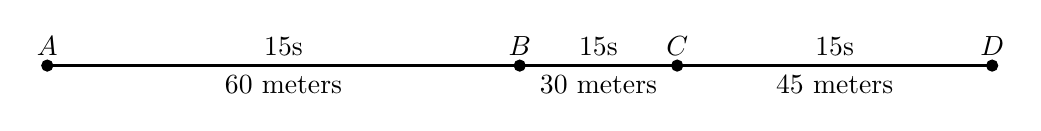
\begin{tikzpicture}
% Define the total length and segment lengths
\def\totalLength{12}
\def\segmentOne{6}   % 15s segment
\def\segmentTwo{2}   % 5s segment  
\def\segmentThree{4} % 10s segment

% Draw the main line
\draw[thick] (0,0) -- (\totalLength,0);

% Define the points
\coordinate (A) at (0,0);
\coordinate (B) at (\segmentOne,0);
\coordinate (C) at (\segmentOne+\segmentTwo,0);
\coordinate (D) at (\totalLength,0);

% Draw solid points at A, B, C, D
\foreach \point/\label in {A/A, B/B, C/C, D/D} {
    \filldraw[black] (\point) circle (2pt);
    \node[above] at (\point) {$\label$};
}

% Add time labels above the segments
\node[above] at ($(A)!0.5!(B)$) {15s};
\node[above] at ($(B)!0.5!(C)$) {15s};
\node[above] at ($(C)!0.5!(D)$) {15s};

% Optional: Add distance markers below the line
\node[below] at ($(A)!0.5!(B)$) {60 meters};
\node[below] at ($(B)!0.5!(C)$) {30 meters};
\node[below] at ($(C)!0.5!(D)$) {45 meters};


\end{tikzpicture}
  \end{center}
  \begin{enumerate}
    \item
	What is the formula of harmonic mean? \hfill 1
    \item
	When should we use the harmonic mean? \hfill 2
    \item  
	Find the average velocity of the vehicle. \hfill 3
    \item
	Compare the average speed estimated using the arithmetic and harmonic mean and \\ verify their suitability in the given situation. \hfill 4
  \end{enumerate}


 \item
	  \textbf{While driving from city A to city B, a car got 22 miles per gallon and
while returning on the same road, the car got 30 miles per gallon.} 
  \textcolor{red}{REVIEW THE QUESTION}
  \begin{enumerate}
    \item
	How many measures of centrtal tendencies are there? \hfill 1
    \item
	Which route takes more amount of fuel per mile? \hfill 2
    \item  
	If the total distance for the round trip was 300 miles, how many gallons of fuel were used for the entire journey? \footnote{$$\frac{150}{22} + \frac{150}{30} \text{ gallons} = \frac{130}{11} \text{ gallons} = 11.82 \text{ gallons}$$} \hfill 3
    \item
	Find the car’s average gas mileage for the entire trip, in miles per gallon. \hfill 4
  \end{enumerate}

     \item
	  \textbf{A shrimp producer wanted to get an insight into his shrimp production. To do so, he randomly collected weights of different shrimps in his farm.} 
	  

	  \begin{table}[h]
	  \centering
\begin{tabular}{c|c|c|c|c|c}
Weight of shrimp (gm) & 10-20 & 20-30 & 30-40 & 40-50 & 50-60 \\ \hline
Frequency & 5 & 8 & 10 & 9 & 4
\end{tabular}
\end{table}

  \begin{enumerate}
    \item
	What is the primary goal of central tendency?\hfill 1
    \item
	When is Median a better measure of central tendency than Arithmetic Mean and why? \hfill 2
    \item  
	From the stem, find 3rd quartile and explain. \hfill 3
    \item
	Find harmonic mean (HM) and compare with the arithmetic mean (AM) \hfill 4
  \end{enumerate}

 \item
	  \textbf{An arithmetic series is formed as follows:}
	  
	   \begin{center}
  \textbf{$a, a+c, a+2c, \cdots, a+2nc$}
  \end{center}
  
  \begin{enumerate}
    \item
	What is change of origin and scale? \hfill 1
    \item
	Convert the series into a set of natural numbers. \hfill 2
    \item  
	Find the arithmetic mean of the series with the use of change of origin and scale. \hfill 3
    \item
	Find the geometric mean of the series: $1, 2, 4, \cdots , 2^n$ . \hfill 4
  \end{enumerate}

 \item
	  \textbf{Scores by Travis Head in the last two matches of ICC Men's 
	  Cricekt World - 2023 are given. In Cricket, Strike Rate (SR) is computed by dividing Runs by Balls and then multiplying the quotient by 100.} 
	  
	  \begin{table}[h]
	  \centering
\begin{tabular}{c|c|c}
Match & Runs & Balls \\ \hline 
1 & 62 & 48 \\
2 & 137 & 120 \\ \hline 
\end{tabular}
\end{table}
  
  \begin{enumerate}
    \item
	How many averages do you know of? \hfill 1
    \item
	Give an example when arithmetic mean is appropriate instead of harmonic mean. \hfill 2
    \item  
	When is Weighted Harmonic mean is used. Show a numerical example. \hfill 3
    \item
	Determine the average Strike Rate of the batter \hfill 4
  \end{enumerate}
  
   \item
	  \textbf{Average height of the four tallest towers in Dhaka is 153.25 meters. The heights of first three towers is 171, 153 and 152 meters, respectively. A new tower has been built with height 150 meters.} 
  
  \begin{enumerate}
    \item
	Write two primary uses of central tendency. \hfill 1
    \item
	Prove mathematically: $\displaystyle \sum_{i=1}^n (x_i-\bar x) = 0$ \hfill 2
    \item  
	Compute the height of the forth tower. \hfill 3
    \item
	After the addition of the new tower, will the average increase or decrease? Explain logically and empirically (using data). \hfill 4
  \end{enumerate}

 \item
	  \textbf{For two non-zero positive numbers, $GM=4\sqrt3$ and $HM=6$, where the quantities bear usual notations} 
  
  \begin{enumerate}
    \item
	When is Harmonic mean suitable? \hfill 1
    \item
	For two numbers, what is the relationship between AM, GM, and HM? \hfill 2
    \item  
	What is the Arithmetic mean? \hfill 3
    \item
	Determine the numbers. \hfill 4
  \end{enumerate}
  
  \item
\textbf{For two positive non-zero numbers, if $GM = 5\sqrt{2}$ and $AM = 8$, where the symbols represent their usual meanings:}

\begin{enumerate}
    \item  
    Find the Harmonic mean (HM). \hfill 3
    \item
    Identify the two numbers. \hfill 4
\end{enumerate}

\item
\textbf{For two positive non-zero numbers, if $GM = 6\sqrt{3}$ and $AM = 10$, where the symbols represent their usual meanings:}

\begin{enumerate}
    \item  
    Determine the Harmonic Mean (HM) of the two numbers. \hfill 3
    \item
    Find the values of the two numbers. Comment on the obtained values. \hfill 4
\end{enumerate}

  
   \item
	  \textbf{12 is deducted from each value of a variable and then divided by 3. The new arithmetic mean (AM) is found to be 4.} 
  
  \begin{enumerate}
    \item
	What is change of origin? \hfill 1
    \item
	Does AM depend on origin? Prove with an example. \hfill 2
    \item  
	From the stem, find the original AM. \hfill 3
    \item
	Does the origin or the scale have greater impact on AM in this example? \hfill 4
  \end{enumerate}
  
   \item
	  \textbf{A statistics teacher gave a test to students worth 50 marks. After publishing the result, it was decided the marks would be converted to 100-marks scale. It was also noted that each student should get 2 marks more than the given marks.} 
  
  \begin{enumerate}
    \item
	In the stem, which concept is revealed? \hfill 1
    \item
	Does the arithmetic mean depend upon change of scale? \hfill 2
    \item  
	Demonstrate the effect of change of origin and scale on arithmetic mean, deriving the formula for conversion between them. \hfill 3
    \item 
    If the original arithmetic mean of the marks of the students is 44, what is the changed mean? Does the change of origin and scale always increase the value? Analyze.
	 \hfill 4
  \end{enumerate}

   \item
	  \textbf{The arithmetic and geometric means of ages two boys Abir and Abid are 10 and 8.} 
  
  \begin{enumerate}
    \item
	What is arithmetic mean? \hfill 1
    \item
	When can we not calculate arithmetic mean? \hfill 2
    \item  
	Determine the ages of Abir and Abid. \hfill 3
    \item
	Does the data comply with the theorem $\displaystyle AM \times  = GM^2$? \hfill 4
  \end{enumerate}
  
     \item
	  \textbf{Income of 100 individuals in the city of Rajshahi were analyzed and found to produce the the following distribution:} 
	  
	  \begin{table}[h]
	  	  \centering
\begin{tabular}{c|ccccc}
Income                                                           & 40-50 & 50-60 & 60-70 & 70-80 & 80-90 \\ \hline
\begin{tabular}[c]{@{}c@{}}Number of \\ Individuals\end{tabular} & 15    & 20    & 35    & 20    & 10   
\end{tabular}
\end{table}
  
  \begin{enumerate}
    \item
	What is Median? \hfill 1
    \item
	Does median necessarily lie in the dataset? \hfill 2
    \item  
	Estimate Median and explain the result. \hfill 3
    \item
	Find Arithmetic Mean and Mode. Which measure seems to be the best one? \hfill 4
  \end{enumerate}
  
   \item
	  \textbf{Amount of rainfall in some cities around the world for a month were obtained as follows:} 
	  
	      \begin{table}[h]
    \centering
\begin{tabular}{c|c}
\textbf{Rainfall (mm)} & \textbf{Frequency} \\ \hline
20-30                  & 5                  \\ \hline
30-40                  & 6                  \\ \hline
40-50                  & 4                  \\ \hline
50-60                  & 3                  \\
60-70                  & 5                 
\end{tabular}
\end{table}

    \begin{enumerate}
    \item
	When is Short-Cut method for Arithmetic Mean useful? \hfill 1
    \item
	Derive the formula of Short-cut Method \hfill 2
    \item  
	Compute the Arithmetic Mean using the Short-cut method. \hfill 3
    \item
	Compute the Arithmetic Mean with a different value of origin (a). Do both the methods give same result?\hfill 4
  \end{enumerate}
  
     \item
\textbf{The number of hours spent studying per week by students in a school were recorded as follows:}

\begin{table}[h]
\centering
\begin{tabular}{c|c}
\textbf{Hours Studied} & \textbf{Frequency} \\ \hline
0-5                   & 8                  \\ \hline
5-10                  & 12                 \\ \hline
10-15                 & 10                 \\ \hline
15-20                 & 6                  \\ \hline
20-25                 & 4                 
\end{tabular}
\end{table}

    \begin{enumerate}
    \item
	Relate short-cut method of arithmetic mean with change of origin and scale. \hfill 2
    \item  
	Compute the Arithmetic Mean of the given data using the short-cut method. \hfill 3
    \item
	Compute the Arithmetic Mean with a different value of origin (a). Do both the methods give same result? What is the best choice of a? \hfill 4
  \end{enumerate}
  
  \item
\textbf{Concentrations of a chemical solution (in mol/L) were recorded over 
several trials as follows:} 

\begin{table}[h]
\centering
\begin{tabular}{c|ccccc}
\textbf{Concentration (mol/L)} & 0.1-0.2 & 0.2-0.3 & 0.3-0.4 & 0.4-0.5 & 0.5-0.6 \\ \hline
\textbf{Frequency}             & 4       & 7       & 5       & 6       & 3       
\end{tabular}
\end{table}

\begin{enumerate}
    \item  
    Compute the Arithmetic Mean using the Short-cut method. \hfill 3
    \item
    Compute the Arithmetic Mean using a different assumed mean (A). \\
    Do both methods yield the same result? \hfill 4
\end{enumerate}

  
     \item
	  \textbf{A sports analyst collected ages of athelets having ages between 10 and 35. He then presented his findings as below:} 
	  
	  \begin{table}[h]
	    \centering
\begin{tabular}{c|c|c|c|c|c}
Age            & 10-15 & 15-20 & 20-25 & 25-30 & 30-35 \\ \hline
No. of Athlete & 2     & 8     & 10    & 5     & 3    
\end{tabular}
\end{table}
  
  \begin{enumerate}
    \item
	What is central tendency? \hfill 1
    \item
	When is geometric mean iappropriate to measure? \hfill 2
    \item  
	Compute median from the stem. \hfill 3
    \item
	Show that Arithmetic mean is greater than Harmonic mean. Which one of them is more suitable for this data? \hfill 4
  \end{enumerate}
  
   \item
  \textbf{The monthly temperatures in the cities of Dhaka (in Degree Celsius) and New York (in degree Fahrenheit) are given in the following table:}
  
  % Please add the following required packages to your document preamble:
% \usepackage[normalem]{ulem}
% \useunder{\uline}{\ul}{}
\begin{table}[h]
\centering
\begin{tabular}{ccccccccccccc}
City             & Jan  & Feb  & Mar  & Apr  & May  & Jun  & Jul  & Aug  & Sep  & Oct  & Nov  & Dec  \\
Dhaka ($^o C)$   & 24.6 & 28.3 & 32.4 & 33.9 & 33.6 & 32.8 & 32.1 & 32.3 & 32.4 & 31.9 & 29.7 & 26.1 \\
New York ($^oF$) & 29   & 32   & 40   & 50   & 60   & 70   & 75   & 74   & 67   & 56   & 46   & 35  
\end{tabular}
\end{table}

  
  \begin{enumerate}
    \item
	How is the Range defined? \hfill 1
    \item
	Can the standard deviation exceed the variance? Prove. \hfill 2
    \item  
	Find the standard deviation of the above data and compare the cities. \hfill 3
    \item
	Examine the efficacy the standard deviation in light of the given context. Is a better measure availabe? Analyze. \hfill 4
  \end{enumerate}

   \item
	  \textbf{Mean monthly salaries of employees of two companies A \& B are tk. 
	  65,000 and tk. 75,000. The combined arithmetic mean (AM) is tk. 
	  71,000 and number of employees in the company A is 20.} 
	  
  \begin{enumerate}
    \item
	Write down the formula of combined AM for k groups. \hfill 1
    \item
	What is the combined AM of two data sets with AM 35 and 45 and number of values equal? \hfill 2
    \item  
	How many employees are there in the company B? \hfill 3
    \item
	Salary of an employee of company A was recorded as tk. 60,000 in place of
	65,000. What is the new AM of company A. Also find the corrected combined AM.\hfill 4
  \end{enumerate}
  
  \item
\textbf{Average marks of two sections A \& B in a statistics exam are 68 and 74 respectively. The overall average mark of both sections combined is 70. Section A has 25 students.}

\begin{enumerate}
    \item  
    How many students are there in section B? \hfill 3
    \item
    Later, it was found that a student in section B was wrongly marked 80 instead of 90. Find the corrected average of section B and the new combined average. \hfill 4
\end{enumerate}


     \item
	  \textbf{A departmental store records their sales. An analysis of products with prices less than tk. 30 generates the following table.} 
	  
\begin{table}[H]
\centering
\begin{tabular}{c|c|c|c|c|c|c}
Price     & 0-5 & 5-10 & 10-15 & 15-20 & 20-25 & 25-30 \\ \hline
Frequency & 1   & 0    & 2     & 3     & 8     & 12   
\end{tabular}
\end{table}
  
  \begin{enumerate}
    \item
	What is relative frequency? \hfill 1
    \item
	If $Y = a + bX$, $\bar Y = ?$ \hfill 2
    \item  
	Find 67th Percentile and 3rd Quartile and explain. \hfill 3
    \item
	Is AM or Median more suitable for this data? Elucidate. \hfill 4
  \end{enumerate}

   \item
	  \textbf{Arithmetic (AM) and Harmonic Mean (HM) of two numbers are 25 and 9, respectively.} 
    \begin{enumerate}
    \item
	When is HM useful? \hfill 1
    \item
	Derive HM formula using the concept of average velocity. \hfill 2
    \item  
	Find the two values from the stem. \hfill 3
    \item
	Show mathematically that $HM \le AM$ (for n=2) \hfill 4
  \end{enumerate}

   \item
  \textbf{Frequency distribution of marks in statistics of a college is given in the following table.}
 

\begin{table}[h]
\centering
\begin{tabular}{c|c|c}
\hline
Marks & \begin{tabular}[c]{@{}c@{}}Number of Students\\ Group - A\end{tabular} & \begin{tabular}[c]{@{}c@{}}Number of Students\\ Group - B\end{tabular} \\ \hline
25-30 & 11 & 10 \\ \hline
30-35 & 18 & 16 \\  \hline
35-40 & 21 & 22 \\ \hline
40-45 & 26 & 28 \\ \hline
45-50 & 14 & 9 \\ \hline
\end{tabular}
\end{table}

  \begin{enumerate}
    \item
	What is data? \hfill 1
    \item
	What are the disadvantages of secondary data? \hfill 2
    \item  
	Calculate the arithmetic mean of Group - A \hfill 3
    \item
	Compute the combined mean. Is it greather than the arithmetic mean of Group - B? Explain the possible reason(s). \hfill 4
\end{enumerate}

\item  
  \textbf{The following table presents the distribution of monthly salaries (in thousand BDT) of employees in two different departments of a company.}  

\begin{table}[h]
\centering
\begin{tabular}{ccc}
\hline
Salary Range (in 1000 BDT) & \begin{tabular}[c]{@{}c@{}}Number of Employees\\ Department - X\end{tabular} & \begin{tabular}[c]{@{}c@{}}Number of Employees\\ Department - Y\end{tabular} \\ \hline
20-25 & 8 & 6 \\ 
25-30 & 14 & 12 \\ 
30-35 & 19 & 21 \\ 
35-40 & 24 & 26 \\ 
40-45 & 15 & 10 \\ \hline
\end{tabular}
\end{table}

  \begin{enumerate}
    \item  
	Determine the arithmetic mean salary of employees in Department - X.  \hfill 3  
    \item  
	Compute the combined mean salary. Is it higher than the arithmetic mean of Department - Y? Justify your answer with a statistical explanation.  \hfill 4  
\end{enumerate}  



    \item
  \textbf{In the test examination, marks of 11 students in statistics are: 90, 92, 93, 49, 44, 88, 80, 58, 83, 71, 76.}
  \begin{enumerate}
    \item
	What is central tendency? \hfill 1
    \item
	When is median better than arithmetic mean? Explain with an example. \hfill 2
    \item  
	Find the 3rd the quartile and $61^{st}$ percentile from the data and explain.  \hfill 3
    \item
	Do quantiles depend on change of origin and scale. Prove using two examples.\hfill 4
\end{enumerate}

 \item
	  \textbf{HSC exam result of two colleges in a village are given below:} 
	  
	  \begin{table}[h]
	  \centering
\begin{tabular}{c|c|c}
College & Students & Passed \\ \hline
1 & 10 & 8 \\ \hline
2 & 20 & 5
\end{tabular}
\end{table}
  
  \begin{enumerate}
    \item
	How many measures of central tendency are there? \hfill 1
    \item
	Which measure of central tendency is perfect? \hfill 2
    \item  
	Find the pass rate of the colleges and, using them, of the village. \hfill 3
    \item
	Show an alternative method which gives the same result. \hfill 4
  \end{enumerate}

      \item
  \textbf{Scores of a batsman in the last 20 innings are} 
   \begin{center}
  	 28, 30, 16, 48, 50, 86, 105, 20, 10, 36, \\
  	 12, 25, 20, 35, 65, 12, 10, 76, 55, 32
  	 \end{center}
  \begin{enumerate}
    \item
	Write down the formula of weighted harmonic mean \hfill 1
    \item
	Can median be a better measure of central tendency than arithmetic mean for this data?  \hfill 2
    \item  
	Draw a stem and leaf plot from the data and explain.  \hfill 3
    \item
	Make a frequency distribution from the data and also find and interpret cumulative  \hfill 4 \\ frequencies and percentages.
\end{enumerate}

 \item
	  \textbf{In ODI cricket, two top batsmen are (as of 2nd Sept, 2022) Babar Azam and Rassie van der Dussen. Their average (arithmetic mean) scores are 59.79 and 69.32, appearing in 90 (including being not out in 12 occassions) and 33 (including being not out in 11 occassions) matches, respectively.} 
  
  \begin{enumerate}
    \item
	When is arithmetic mean inappropriate to use? \hfill 1
    \item
	Is arithmetic mean always suitable for comparison? \hfill 2
    \item  
	Find the combined arithmetic mean and explain. \hfill 3
    \item
	How to compare two sets of data having significantly distinct ranges? \hfill 4
  \end{enumerate}
  
   \item
	  \textbf{A fridge manufacturing company observe temperatures of newly developed 8 deep fridges. The observed temperatures (in degree celsius are:} 
	  
	    \begin{center}
-10, -8, -2, -4, -4, -1, -12, -3, -13
  \end{center}
  
  \begin{enumerate}
    \item
	What is a Decile? \hfill 1
    \item
	How many Deciles does a data set have? Why? \hfill 2
    \item  
	Compute the 8th Decile from the data and explain. \hfill 3
    \item
	What is the value below which 75\% observations lie? Find in two distinct ways. \hfill 4
  \end{enumerate}
  
   \item
	  \textbf{Given below is a series of data.} 
	  
	  	    \begin{center}
	 $5, 7, 9, \cdots , 123$
	    \end{center}
  
  \begin{enumerate}
    \item
	What is the summation of natural numbers up to nth value? \hfill 1
    \item
	Find the arithmetic mean of natural numbers from 1 up to 20. \hfill 2
    \item  
	Find the arithmetic mean of the given series. \hfill 3
    \item
	Prove that arithmetic mean is greater than gemetric mean theoretically and empricially. \hfill 4
  \end{enumerate}
  
   \item
	  \textbf{Grades of a an undergraduate student with major in statistics are given below: } 
	  
	  [Credits serve as weights]

\begin{table}[h]
\centering
\begin{tabular}{c|c|c|c|c|c|c}
\hline
Course & Probability & Simulation & Calculus & Linear Algebra & Econometrics & Programming \\ \hline
Grade & 3.75 & 3.50 & 3.50 & 3.75 & 3.00 & 3.50 \\  \hline
Credit & 4 & 3 & 4 & 4 & 2 & 3 \\ \hline
\end{tabular}
\end{table}


  \begin{enumerate}
    \item
	Write down the formula of weighted mean. \hfill 1
    \item
	What is difference between weight and frequency? \hfill 2
    \item  
	Determine the GPA of the student. \hfill 3
    \item
	Determine the geometric mean for the data and evaluate \\ suitability. \hfill 4
  \end{enumerate}

 \item
	  \textbf{A student walks 3 hours at 5 km per hour (kph), 4 hours at 4 kph, and 2 hours at 3 kph.} 
  
  \begin{enumerate}
    \item
	When is harmonic mean suitable? \hfill 1
    \item
	Which mean could we use for the given data and why? \hfill 2
    \item  
	Find the average speed using weighted harmonic mean. \hfill 3
    \item
	Find the correct and suitable average speed using another method and mathematically show they are equivalent. \hfill 4
  \end{enumerate}
  
  \item
    \textbf{Scores of four athletes in different events at a track meet are recorded below:}

\begin{table}[h]
\centering
\begin{tabular}{c|c|c|c|c}
\hline
Event & High Jump & Long Jump & Shot Put & Javelin Throw \\ \hline
Score & 8.5 & 7.2 & 12.8 & 55.5 \\ \hline
Difficulty Factor & 2 & 3 & 2.5 & 1.5 \\ \hline
\end{tabular}
\end{table}

\textbf{A coach believes that events with higher difficulty factors should contribute more to the overall ranking and suggested a new weighting where the weight for each event is the square of its difficulty factor.}

  \begin{enumerate}
    \item
	Write down the formula of weighted mean. \hfill 1
    \item
	What is difference between weight and frequency? \hfill 2
	 \item Calculate the weighted average score of the athletes across all four events. \hfill 3
    \item If the coach's suggestion is implemented, would the mean be shifted upward or downward? Show mathematically and empricially. \hfill 4
  \end{enumerate}
  
  \item
\textbf{A biologist observes three different species of fish swimming at 
different speeds. The recorded swimming speeds are 2 m/s for 4 hours, 
3 m/s for 3 hours, and 5 m/s for 2 hours.}

\begin{enumerate}
    \item  
    Find the average swimming speed using the weighted harmonic mean. \hfill 3
    \item
    Confirm the average speed by applying another method and prove their 
    mathematical equivalence. \hfill 4
\end{enumerate}

\item
\textbf{A biologist records the lengths (in cm) of a certain species of 
fish found in different water bodies as shown below:}

\begin{table}[h]
\centering
\begin{tabular}{c|c|c|c|c|c}
\textbf{Category} & 5-10 & 10-15 & 15-20 & 20-25 & 25-30 \\ \hline
\textbf{Frequency} & 8    & 12    & 15    & 10    & 5     
\end{tabular}
\end{table}

\begin{enumerate}
    \item  
    Compute the Arithmetic Mean of the fish lengths. \hfill 3
    \item
    Suppose there is another set of data from a similar study with a mean of 17 cm and 20 observations. Find the combined mean of the two datasets and compare it with the mean found in (i). \hfill 4
\end{enumerate}

 \item
	  \textbf{A meteorologist records the monthly rainfall (in mm) in different regions over a year as shown below:}

\begin{table}[h]
\centering
\begin{tabular}{c|c|c|c|c|c}
\textbf{Rainfall (mm)} & 0-50 & 50-100 & 100-150 & 150-200 & 200-250 \\ \hline
\textbf{Frequency}     & 6    & 10     & 14      & 8       & 7       
\end{tabular}
\end{table}

  
  \begin{enumerate}
    \item
	Which class contains the Mode? \hfill 1
    \item
	Find $\Delta_1$ and $\Delta_2$, where the symbols represent their usual meanings \hfill 2
    \item  
	Find the Mode using the Direct formula. \hfill 3
    \item
	Find the Mode using histogram and compare with direct method. \\ Which one do you think is more accurate? \hfill 4
  \end{enumerate}
  
  
   \item
	  \item
\textbf{An ecologist records the number of trees in different forest plots based on their heights (in meters) over a survey period as shown below:}

\begin{table}[h]
\centering
\begin{tabular}{c|c|c|c|c|c}
\textbf{Tree Height (m)} & 0-5 & 5-10 & 10-15 & 15-20 & 20-25 \\ \hline
\textbf{Frequency}       & 5   & 12   & 18    & 9     & 6      
\end{tabular}
\end{table}

  
  \begin{enumerate}
    \item
	How much data lie below the Median point? \hfill 1
    \item
	What is the relationship between the median and the quartiles? \hfill 2
    \item  
	Find the median using the direct formula. \hfill 3
    \item
	Find the 1st and 3rd quartile from the table and interpret. \hfill 4
  \end{enumerate}
  
  \textcolor{red}{ADD QUESTIONS ASKING MODE AND MEDIAN AND OTHER QUARTILES FROM GRAPH}

\item
\textbf{A botanist measures the heights (in cm) of plants from a sample as shown below:}

\begin{table}[h]
\centering
\begin{tabular}{c|c|c|c|c|c}
\textbf{Height (cm)} & 20-30 & 30-40 & 40-50 & 50-60 & 60-70 \\ \hline
\textbf{Frequency} & 6 & 10 & 12 & 8 & 4
\end{tabular}
\end{table}

\begin{enumerate}
    \item  
    Find the median height of the plants and interpret. \hfill 3
    \item
    Determine the first (Q1) and third (Q3) quartiles of the plant heights. Explain the significance of these quartiles in understanding the data distribution. \hfill 4
\end{enumerate}

  
   \item
	  \textbf{A passer-by walks 3 hours at 5 km per hour (kph), another 3 hours 
	  at 4 kph, and another 3 hours at 3 kph.} 
  
  \begin{enumerate}
    \item
	When is harmonic mean suitable? \hfill 1
    \item
	Which mean could we use for the given data and why? \hfill 2
    \item  
	Find the average speed of the passer-by usingt he proper method. \hfill 3
    \item
	Find the correct and suitable average speed using another method and mathematically show they are equivalent. \hfill 4
  \end{enumerate}

 \item
	  \textbf{A cyclist moves around a square-shaped lake with the speeds 20, 25, 30, and 16 km per hour.} 
  
  \begin{enumerate}
    \item
	What is grouped data? \hfill 1
    \item
	Is arithmetic mean suitable for this data? \hfill 2
    \item  
	Find the average speed of the cyclist. \hfill 3
    \item
	Can we use some other formula for finding the same value of the average? Demonstrate. \hfill 4
  \end{enumerate}
  
     \item
	  \textbf{There are only two students in a class IX in a college. In half-yearly exam, the arithmetic and the geometric mean of the marks of those two studnets are 25 and 15, respectively.} 
  
  \begin{enumerate}
    \item
	Write down the formula of Geometric Mean for grouped data. \hfill 1
	\item Prove with an example: $\displaystyle \sum_{i=1}^n (x_i-\bar x) = 0$ \hfill 2
    \item  
	Determine the marks of the students. \hfill 3
    \item
	Is 20 a possible value of the harmonic mean of this data? Explain theoretically and empirically. \hfill 4
  \end{enumerate}

\begin{table}[h]
\centering
\begin{tabular}{c|c|c|c|c|c}
\textbf{Rainfall (mm)} & 20-30 & 30-40 & 40-50 & 50-60 & 60-70 \\ \hline
\textbf{Frequency} & 5 & 6 & 4 & 3 & 5
\end{tabular}
\end{table}

\item
\textbf{Five judges mark a participant in a competition. A more experienced judge's mark carries a larger weight, as shown below:}
\begin{center}
\begin{tabular}{l|c|c|c|c|c}
Judge & 1 & 2 & 3 & 4 & 5 \\ \hline
Mark ($x$) & 2 & 4 & 6 & 7 & 9 \\ \hline
Weight ($w$) & 3 & 2.5 & 2 & 1.5 & 1
\end{tabular}
\end{center}
\begin{enumerate}
  \item Write down the formula of the weighted arithmetic mean. \hfill 1
  \item Why is a weighted mean more suitable than a simple mean here? \hfill 2
  \item Find the weighted arithmetic mean of the marks. \hfill 3
  \item The organisers consider giving all the judges equal weight. Would the participant benefit? Justify with calculations. \hfill 4
\end{enumerate}

\item
\textbf{The scores of a student in six courses, along with the credits of the courses, are given below:}
\begin{center}
\begin{tabular}{l|c|c|c|c|c|c}
Course & Math & English & Art & Physics & ICT & History \\ \hline
Score ($x$) & 90 & 80 & 70 & 85 & 75 & 62 \\ \hline
Credit ($w$) & 4 & 3 & 2 & 4 & 2 & 1
\end{tabular}
\end{center}
\begin{enumerate}
  \item When is the weighted arithmetic mean equal to the simple arithmetic mean? \hfill 1
  \item Find the simple arithmetic mean of the scores. \hfill 2
  \item Find the weighted arithmetic mean of the scores, using the credits as weights. \hfill 3
  \item The student claims that 10 more marks in Art would raise the weighted mean as much as 10 more marks in Math. Verify the claim. \hfill 4
\end{enumerate}


\item
\textbf{The number of bacteria (in thousands) in a culture was counted at the end of five successive hours:}
\begin{center}
\begin{tabular}{l|c|c|c|c|c}
Hour & 1 & 2 & 3 & 4 & 5 \\ \hline
Bacteria ($x$) & 3 & 6 & 12 & 24 & 48
\end{tabular}
\end{center}
\begin{enumerate}
  \item Write down the formula of the geometric mean for ungrouped data. \hfill 1
  \item What happens to the geometric mean if one of the values is 0? Explain. \hfill 2
  \item For $n$ positive values, derive the formula $\displaystyle G = \mbox{antilog}\left(\frac{1}{n}\sum_{i=1}^{n} \log x_i\right)$. \hfill 3
  \item Find the geometric mean of the data directly and by using logarithm and antilogarithm, and compare the results. \hfill 4
\end{enumerate}

\item
\textbf{The monthly savings (in hundred taka) of 40 families are given below:}
\begin{center}
\begin{tabular}{l|c|c|c|c|c}
Savings & 0-10 & 10-20 & 20-30 & 30-40 & 40-50 \\ \hline
No. of families & 4 & 8 & 15 & 9 & 4
\end{tabular}
\end{center}
\begin{enumerate}
  \item Write down the formula of the geometric mean for grouped data. \hfill 1
  \item The first class starts at 0. Does this prevent us from finding the geometric mean? Explain. \hfill 2
  \item Find the geometric mean of the savings using logarithm and antilogarithm. \hfill 3
  \item Find the arithmetic mean of the savings and, comparing it with the geometric mean, comment on the relation between the two. \hfill 4
\end{enumerate}

% MGCC 43 pre-test 2026
\item
\textbf{The yields (in kg) of 100 mango trees in an orchard in Rajshahi have the following distribution:}
\begin{center}
\begin{tabular}{l|ccccc}
Yield (kg) & 20--30 & 30--40 & 40--50 & 50--60 & 60--70 \\ \hline
Number of trees & 12 & 22 & 36 & 18 & 12
\end{tabular}
\end{center}
\begin{enumerate}
  \item What is the median? \hfill 1
  \item Does the median necessarily lie in the data set? Explain. \hfill 2
  \item Estimate the median and explain the result. \hfill 3
  \item Find the arithmetic mean and the mode. Which measure seems to be the best one? \hfill 4
\end{enumerate}

% MGCC 43 pre-test 2026
\item
\textbf{In an auditorium, the first row has 8 seats and each following row has 3 more seats than the row before it. The numbers of seats in the rows are:}
\begin{center}
$8, 11, 14, \cdots, 125$
\end{center}
\begin{enumerate}
  \item What is the sum of the first $n$ natural numbers? \hfill 1
  \item Find the arithmetic mean of the natural numbers from 1 to 30. \hfill 2
  \item Find the average number of seats per row. \hfill 3
  \item Prove that the arithmetic mean of two unequal positive values is greater than their geometric mean, and verify it using the numbers of seats in the first and last rows. \hfill 4
\end{enumerate}

\end{enumerate}

\section{Short Questions}

\begin{enumerate}

\subsection{General Questions}

    \item What is the primary purpose of central tendency? \hfill 1
    \item When is WAM equal to WHM? Show mathematically. \hfill 2
    \item When is the equality true: $AM=GM=HM$? Prove mathematically and empirically.  \hfill 3
    \item When is Median a better measure of central tendency than Arithmetic Mean?  \hfill 1
    \item When is Harmonic Mean more suitable than Arithmetic Mean?  \hfill 1
    \item Write two primary uses of central tendency. \hfill 1
    \item For two distinct non-zero values, what is the relationship among AM, GM, and HM? \hfill 1
    \item what is the relationship among AM, GM, and HM? \hfill 1
    \item What are the criteria of a good measure of central tendency? \hfill 1
    \item For two non-zero positive numbers, prove $AM \ge GM \ge HM$ \hfill 3
    \item Find the AM, GM, and HM: $1,2,4,\cdots, 2^n$ \hfill 4
    \item A data set has the following values: 5, 10, 20, 30. Find AM, GM, HM, Median, and Mode and order the results in ascending order. \hfill 4

    
\subsection{Arithmetic Mean}

    \item Does Arithmetic Mean depend on change of origin and 
    scale? Prove mathematically and with an example. \hfill 3
    \item If $\bar{X} = 3 , \text{ and } n = 10$, what is $\sum X_i$? \hfill 2
    \item Derive the formula of combined mean using logic and an example. \hfill 2
    \item Prove with an example: $\displaystyle \sum_{i=1}^n (x_i-\bar x) = 0$ \hfill 2
    \item Prove mathematically: $\displaystyle \sum_{i=1}^n (x_i-\bar x) = 0$ \hfill 2
    \item Derive the formula of Arithmetic Mean for short-cut method. \hfill 2
    \item Derive the formula of combined Arithmetic Mean for $n$ nnumber of observations.
    \item Find Arithmetic Mean of first n natural numbers. \hfill 2
    \item If $u_i = x_i + y_i$, find $\bar x$ in terms of $u$. \hfill 1
    \item For two numbers, $AM=25$ and $GM=15$. $HM=?$ \hfill 1
    \item $\bar X = 25$ and $Y_i = 5X_i + 20$. $\bar Y = ?$
    \item Find Arithmetic Mean: $11,13,15, \cdots, 57$
    \item Find Arithmetic Mean: $115,120,125, \cdots, 225$
    \item Find Arithmetic Mean: $14,18,22, \cdots, 70$ \hfill 2
    \item Find Arithmetic Mean: $0, 5, 10, \cdots, 70$ \hfill 2
    \item Arithmetic Mean ($\bar X$) of five numbers is 40, and of three of them is 30. What is $\bar X$ of the rest two?
    \item AM of 200 values is found to be 50. Later it was seen two values were recorded as 92 and 8 in place of 192 and 88, respectively. What is the correct AM?
    \item AM of 8 values of 20. If the 9th value is 0, what is the new AM?
    \item AM of Income of City A is 1500 and of City B is 1200. If a person moves from city A to city B, can AM of both cities decrease?
    \item Calculate Arithmetic Mean:
    
    \begin{table}[h]
    \centering
\begin{tabular}{c|c}
\textbf{Renumeration (X)} & \textbf{No. of Employees (f)} \\ \hline
30               & 5                    \\ \hline
35               & 8                    \\ \hline
40               & 10                  
\end{tabular}
\end{table}
    
    \item Calculate Arithmetic Mean using short-cut method:
    
    \begin{table}[h]
    \centering
\begin{tabular}{c|c}
\textbf{Rainfall (mm)} & \textbf{Frequency} \\ \hline
20-30                  & 5                  \\ \hline
30-40                  & 6                  \\ \hline
40-50                  & 4                  \\ \hline
50-60                  & 3                  \\
60-70                  & 5                 
\end{tabular}
\end{table}

    \item What is the relationship between changing origin \& scale and short-cut method of Arithmetic Mean?

\subsection{Geometric Mean}    
    \item Write down the formula of Geometric Mean for grouped data.
    \item Find Geometric Mean for these values: $2, 4, 8$ \hfill 1
    \item Derive the formula of Geometric Mean using logarithm. \hfill 1
    \item When is Geometric Mean not calculable? \hfill 1
    \item When is Geometric Mean appropriate? \hfill 1
    \item Determine the formula of combined Geometric Mean when $n_1=n_2=n$ \hfill 1
    \item $Y_i = 3X_i$. If $G_y = 9, G_x=?$ [G stands for Geometric Mean] \hfill 2
    \item $n_1=15, G_1=75, n_2=10, \space and \space G_2=80$ Find combined GM.

\subsection{Harmonic Mean}

    \item Write down the formula of Weighted Harmonic Mean.\hfill 1
    \item When is Weighted Harmonic Mean used instead of Unweighted one? \hfill 1
    \item Calculate Harmonic Mean: $10,15,20$ \hfill 1
    \item Show mathematically that Harmonic Mean of velocity for a fixed distance is equal to average velocity.
    \item Find the average speed:
    
    \begin{table}[h]
    \centering
\begin{tabular}{c|c|c}
Path   & Distance (km) & Speed (km/h) \\ \hline
Path 1 & 3             & 8            \\ \hline 
Path 2 & 2             & 9            \\ \hline
Path 3 & 2             & 2           
\end{tabular}
\end{table}

\subsection{Median}

    \item Does Median depend on origin and scale? Prove with an example?
    \item How much data lie below the Median point? \hfill 1
    \item What is the relationship between the median and the quartiles? \hfill 2
    \item Median score of 50 students is 70. What does it mean? \hfill 1
    \item Write down the formula of Median for even number of observations.
    \item Write down the formula of Median for grouped data. 
    \item Find median: $5,10, 15, 20, 25, 30$
    \item Find median: $7,  2,  4,  5,  6, 10$ and explain the value \hfill 2
    \item Is Median affected by outliers?
    \item Does Median depend on origin and scale? Prove. \hfill 2
    \item What is the greatest disadvantage of Median?
    \item Does Median always lie in the data set from which it is calculated? \hfill 1
    
\subsection{Mode}

    \item What is the formula of Mode for grouped data?
    \item Find the mode: $2,2,3,3,4,4,2,2,7$
    \item What is an Unimodal dataset?

\subsection{Quadratic Mean}

    \item What is the formula of Quadratic Mean for grouped and ungrouped data?
    \item When is Quadratic Mean used?

\subsection{Partition Values}
    \item If a data is divided into four parts, how many partition values are created?
    \item Write down the formula of Median for even and odd number of observations.
    \item Derive the general formula of Quartiles using the concept of Median?
    \item Third Quartile of score of 50 students is 76. What does it mean?
    \item Which Quartile is equal to Median?
    \item Which Percentile is equal to 3rd Quartile?
    \item Find all the Quartiles and interpret: $2,1,0,5,-6,7,-4$ \hfill 3

    
\end{enumerate}

\chapter{Measures of Dispersion} 
\section{Creative Questions}

\begin{enumerate}

\item
\textbf{Rainfall measurements (in mm) of two cities for six days are as below:}

\begin{table}[h]
\centering
\begin{tabular}{c|cccccc}
Day & 1 & 2 & 3 & 4 & 5 & 6 \\
\hline
City X & 15 & 12 & 10 & 18 & 14 & 11 \\ \hline
City Y & 20 & 8 & 25 & 5 & 22 & 10 \\
\end{tabular}
\end{table}

\begin{enumerate}
    \item
    What is a measure of dispersion? \hfill 1
    
    \item
    Explain with an example why measuring dispersion is important in data analysis. \hfill 2
    
    \item
    Calculate the variance of rainfall for City X. \hfill 3
    
    \item
    Which city shows more consistent rainfall? Justify. \hfill 4
\end{enumerate}

    \item
  \textbf{Temperatures of two cold regions for five days are as below:}

    \begin{center}

    City A: 2, 1, -1, 0, 3

    City B: 3, 0, -2, 2, 3
    
    \end{center}
  \begin{enumerate}
    \item
	What is dispersion? \hfill 1
    \item
	Illustrate the necessity of dispersion with an example. \hfill 2
    \item  
	Find the variance of temperature of city A.  \hfill 3
    \item
	Which city has more consistent temperature? Analyze.\hfill 4
\end{enumerate}

    \item
  \textbf{Temperatures of two cold regions for five days are as below:}

    \begin{center}

    City A: 2, 1, -1, 0, 3

    City B: 3, 0, -2, 2, 3
    
    \end{center}
  \begin{enumerate}
    \item
	What is standard deviation? \hfill 1
    \item
	Is standard deviation of a set of negative values negative? Justify mathematically. \hfill 2
    \item  
	Find Mean Deviation about mean of the values of city A.  \hfill 3
    \item
	Which city has more consistent weather? Verify statistically. \hfill 4
\end{enumerate}

\item  
  \textbf{Rainfall (in mm) recorded in two towns over five days is as follows:}

\begin{table}[h]
\centering
\begin{tabular}{c|ccccc}
Day     & 1  & 2  & 3  & 4  & 5  \\ \hline
Town X  & 12 & 15 & 10 & 18 & 14 \\
Town Y  & 20 & 22 & 18 & 25 & 21
\end{tabular}
\end{table}


  \begin{enumerate}
    \item  
	Find the Mean Deviation about the median for the rainfall data of Town X.  \hfill 3  
    \item  
	Which town shows greater variability in rainfall? Support your answer with statistical measures.  \hfill 4  
\end{enumerate}

\item  
  \textbf{Scores of two students in five tests are as follows:}

\begin{table}[h]
\centering
\begin{tabular}{c|ccccc}
Test     & 1  & 2  & 3  & 4  & 5  \\ \hline
Student A  & 78 & 85 & 90 & 88 & 76 \\ 
Student B  & 80 & 82 & 78 & 86 & 84
\end{tabular}
\end{table}

  \begin{enumerate}
    \item  
	Find the Mean Deviation about the mean for the scores of Student A.  \hfill 3  
    \item  
	Which student has more consistent performance? Justify using statistical measures.  \hfill 4  
\end{enumerate}  

\item  
  \textbf{Monthly sales (in thousand dollars) of two stores over five months are given below:}

\begin{table}[h]
\centering
\begin{tabular}{c|ccccc}
Month     & 1  & 2  & 3  & 4  & 5  \\ \hline
Store P  & 50 & 55 & 48 & 52 & 49 \\
Store Q  & 60 & 58 & 65 & 63 & 61
\end{tabular}
\end{table}

  \begin{enumerate}
    \item  
	Calculate the variance of Store P’s sales data.  \hfill 3  
    \item  
	Compare the sales stability of both stores using an appropriate statistical measure.  \hfill 4  
\end{enumerate}  


 \item
	  \textbf{Two companies A and B pay their workers on a weekly basis. The summary of wages paid by them is shown below:} 
	  
	  \begin{table}[h]
	  \centering
\begin{tabular}{c|ccc}
Factory & Mean Wage (BDT) & Standard Deviation & Number of workers \\ \hline
A       & 1560       & 90                 & 200               \\ 
B       & 1580       & 70                 & 160              
\end{tabular}
\end{table}
  
  \begin{enumerate}
    \item
	What is dispersion? \hfill 1
    \item
	Is variance always greater than stanard deviation? Justify. \hfill 2
    \item  
	Which company is more consistent with their wages? \hfill 3
    \item
	Compare the wages with variance alone. Does it produce the same conclusion. Justify the finding. \hfill 4
  \end{enumerate}
  
  \item 
  \textbf{Two schools, X and Y, conducted the same mathematics examination for their students. The summary of the test scores (out of 100) is shown below:}

\begin{table}[h]
\centering
\begin{tabular}{c|ccc}
School & Mean Score & Standard Deviation & Number of Students \\ \hline
X      & 72.5       & 8.2                & 150                \\ 
Y      & 74.0       & 6.5                & 120               
\end{tabular}
\end{table}

  \begin{enumerate}
    \item  
	Determine the combined standard deviation of the scores of the schools. \hfill 3
    \item
	Which school has more consistent scores? Analyze. \hfill 4
  \end{enumerate}

 \item
	  \textbf{Mean and Standard Deviation of 200 items are found to be 60 and 20. Later it was found that two items were recorded as 3 and 67 in place of 13 and 17.} 
  
  \begin{enumerate}
    \item
	Does standard deviation depend on change of origin? \hfill 1
    \item
	Prove $\displaystyle \sigma^2 = \frac{\sum x^2}n -(\frac{\sum x}{n})^2$ from original formula. \hfill 2
    \item  
	Should the correct mean be smaller or greater? Also find it and compare.  \hfill 3
    \item
	Find the correct standard deviation. \hfill 4
  \end{enumerate}
  
     \item
  \textbf{The monthly temperatures in the cities of Dhaka (in Degree Celsius) and New York (in degree Fahrenheit) are given in the following table:}
  
  
% Please add the following required packages to your document preamble:
% \usepackage[normalem]{ulem}
% \useunder{\uline}{\ul}{}
\begin{table}[H]
\centering
\begin{tabular}{|c|c|c|c|c|c|c|c|c|c|c|c|c|}
\hline
City             & Jan  & Feb  & Mar  & Apr  & May  & Jun  & Jul  & Aug  & Sep  & Oct  & Nov  & Dec  \\ \hline
Dhaka ($^o C)$   & 24 & 28 & 32 & 33 & 33 & 32 & 32 & 32 & 32 & 32 & 29 & 26 \\ \hline
New York ($^oF$) & 29   & 32   & 40   & 50   & 60   & 70   & 75   & 74   & 67   & 56   & 46   & 35   \\ \hline
\end{tabular}
\end{table}

  
  \begin{enumerate}
    \item
	How is the Range defined? \hfill 1
    \item
	Can the standard deviation exceed the variance? Prove. \hfill 2
    \item  
	Find the standard deviation of the above data and compare the cities. \hfill 3
    \item
	Examine the efficacy the standard deviation in light of the given context. \\ Is a better measure availabe? Analyze. \hfill 4
  \end{enumerate}

        \item
  \textbf{  A company recorded the monthly sales (in lakhs of ₹) of two salespersons X and Y for the first half of the year:}


\begin{table}[h]
\centering
\begin{tabular}{c|cccccc}
Month & Jan & Feb & Mar & Apr & May & Jun \\ \hline
Salesperson X & 42 & 38 & 45 & 40 & 43 & 41 \\
Salesperson Y & 50 & 28 & 60 & 35 & 55 & 30
\end{tabular}
\end{table}

\begin{enumerate}
    \item Calculate the \textbf{mean deviation about median} for salesperson X. \hfill 3
    
    \item Which salesperson has \textbf{more consistent sales}? Justify using an appropriate relative measure of dispersion. \hfill 4
\end{enumerate}


      \item
  \textbf{The table below presents the number of goals scored by two footballers, A and B, over five consecutive seasons}

 \begin{table}[h]
\centering
\begin{tabular}{c|c|c|c|c|c}
Season      & 1  & 2  & 3  & 4  & 5  \\ \hline
Footballer A & 10 & 15 & 12 & 9  & 20 \\ \hline
Footballer B & 25 & 5  & 10 & 15 & 6  
\end{tabular}
\end{table}

  \begin{enumerate}
    \item  
	Find Mean Deviation about mean and median of the footballer A.  \hfill 3
    \item
	Which footballer should be hired a club? Determine with the help of a suitable relative measure of dispersion. \hfill 4
\end{enumerate}

% MGCC 43 pre-test 2026
\item
\textbf{Two brands of LED bulbs, A and B, were tested. A summary of their lifetimes is shown below:}
\begin{center}
\begin{tabular}{c|c|c|c}
Brand & Mean lifetime (hours) & Standard deviation (hours) & Number of bulbs \\ \hline
A & 800 & 60 & 50 \\
B & 1200 & 72 & 40
\end{tabular}
\end{center}
\begin{enumerate}
  \item What is dispersion? \hfill 1
  \item Is the variance always greater than the standard deviation? Justify. \hfill 2
  \item Which brand is more consistent in lifetime? \hfill 3
  \item Compare the brands using the variance alone. Does it lead to the same conclusion? Justify the finding. \hfill 4
\end{enumerate}

% MGCC 43 pre-test 2026
\item
\textbf{The mean and standard deviation of the daily output (in units) of 100 workers were found to be 40 and 5. Later it was found that two outputs had been recorded as 30 and 70 in place of 45 and 35.}

\begin{enumerate}
  \item Does the standard deviation depend on a change of origin? \hfill 1
  \item Prove $\displaystyle \sigma^2 = \frac{\sum x^2}{n} - \left(\frac{\sum x}{n}\right)^2$ from the original formula. \hfill 2
  \item Should the correct mean be smaller or greater? Find it and compare. \hfill 3
  \item Find the correct standard deviation. \hfill 4
\end{enumerate}

\end{enumerate}

\section{Short Questions}

 \begin{enumerate}
 
 \item Which measure of dispersion is suitable for an open-ended distribution?  \hfill 1
 \item What does dispersion measure?  \hfill 1
 \item What are the absolute measures of dispersion?
 \item What are the relative measures of dispersion?
 \item What is the formula of Range? \hfill 1
 \item Does Range consider all values? \hfill 1
 \item Is Range influenced by extreme values or outliers? \hfill 1
 \item Write down the formula of Mean Deviation ($MD(\bar x)$.
 \item Write down the formula of Mean Deviation around median ($MD(Me)$.
 \item Write down the formula of Mean Deviation for grouped data ($MD(\bar X)$.
 \item Does mean deviation depend on all values of a dataset? \hfill 1
 \item Does Mean Deviation depend on change of origin and scale? Verify. \hfill 2
  \item When is variance less than standard deviation? \hfill 1
  \item Write down the formula of Quartile Deviation. \hfill 1
 \item Which is the most important measure of dispersion?
   \item Is $\sum |x_i-\bar x|$ always greater than $\sum (x_i-\bar x)$? Prove mathematically. \hfill 2
   \item If $\bar X = 25, CV = 50\%, \sigma^2=?$ \hfill 1
   \item Arithmetic mean of a variable is 16 and variance is 9. What is the value of CV? \hfill 1 
   \item What is the variance of first 5 natural numbers?
 
 \item Find the sum of squares: 12, 10, 11, 15, 20 \hfill 1
 \item Find the square of summation: 2, 5, 7, 8, 4 \hfill 1
 \item Find the sum of squared deviation from the mean of these values: 2, 5, 6, 7, 3 \hfill 1
 \item Find the sum of squares: 8, 6, 9, 12, 14 \hfill 1  

\item Find the square of summation: 3, 7, 5, 9, 6 \hfill 1  

\item Find the sum of squared deviation from the mean of these values: 4, 8, 6, 10, 7 \hfill 1  

\item Compute the sum of squares for the following values: 5, 9, 12, 14, 11 \hfill 1  

\item Compute the square of summation for: 1, 4, 6, 7, 2 \hfill 1  

\item Find the sum of squared deviations from the mean: 3, 6, 8, 10, 5 \hfill 1  

\item Find the sum of squares of differences from 10: 6, 8, 10, 12, 14 \hfill 1  



\subsection{Variance}
\item If $n=10, \sum x_i = 120, \sum x_i^2=2000, CV=?$
\item Is coefficient of variation a pure number? Explain \hfill 2

\end{enumerate}


\chapter{Moments, SKewness, and Kurtosis} 
\section{Creative Questions}

  \begin{enumerate}
  
   \item
	  \textbf{The first four moments around 4 of productions of a company over four years are -1.5, 17, -30, and 108.} 
  
  \begin{enumerate}
    \item
	Can the second central moment be negative? \hfill 2
    \item  
	Determine the second and third central moments. \hfill 3
    \item
	What kind of kurtosis do the data have? \hfill 4
  \end{enumerate}

   \item
	  \textbf{Duration of stays of a spy in foreign countries are obtained by a researcher. As part of an analysis, s/he starts with the following summary.} 
	  
	  \begin{table}[h]
	  \centering
\begin{tabular}{c|cccccc}
Duration & 1-10 & 11-20 & 21-30 & 31-40 & 41-50 & 51-60 \\ \hline
Frequency & 4 & 3 & 3 & 2 & 5 & 2
\end{tabular}
\end{table}
  
  \begin{enumerate}
    \item
	What is symmetry? \hfill 1
    \item
	What is implied by the value of coefficient of skewness 0.8 \hfill 2
    \item  
	Estimate the median of the data and interpret. \hfill 3
    \item
	Obtain coefficient of skewness from data and comment on the life of the spy based on it. \hfill 4
  \end{enumerate}
  
   \item
	  \textbf{The kurtosis and the variance of a symmetrical distribution are $\gamma_2 = -2.3672$ and $\sigma^2 = 4096$, respectively.} 
  
  \begin{enumerate}
    \item  
	Find the fourth central moment. \hfill 3
    \item
	Determine the value of the first and the third raw moments around 5. \hfill 4
  \end{enumerate}
  
  \item  
\textbf{A human resources department recorded the number of years employees have been with the company. The grouped frequency distribution below summarizes the data for a department.}  

\begin{table}[h]
\centering
\begin{tabular}{c|c|c|c|c|c|c}
Years of Service & 0–2 & 3–5 & 6–8 & 9–11 & 12–14 & 15–17 \\ \hline
Frequency & 4 & 6 & 10 & 5 & 3 & 2
\end{tabular}
\end{table}

\begin{enumerate}
  \item  
  Calculate the coefficient of skewness using the grouped data. What does the result indicate about employee tenure? \hfill 3

  \item  
  Compute the coefficient of kurtosis. What does it reveal about the distribution of tenure lengths? \hfill 4
\end{enumerate}

  
  \item  
  \textbf{A financial analyst is studying the annual returns (in percentage) of a set of investment portfolios. The following table summarizes the data.}  

\begin{table}[h]
\centering
\begin{tabular}{c|cccccc}
Annual Return (\%) & -5 to 0 & 1-5 & 6-10 & 11-15 & 16-20 & 21-25 \\ \hline
Frequency & 3 & 5 & 7 & 6 & 4 & 3
\end{tabular}
\end{table}

  \begin{enumerate}
    \item  
	Compute the skewness of the data and interpret the nature of the investment returns.  \hfill 3  
    \item  
	Determine the kurtosis and explain.  \hfill 4  
  \end{enumerate}  



   \item
	  \textbf{There has been an increase in average lifetime of people of Bangladesh. To get more insight on this, a research was conducted, in which ages of retired government employees were recorded. A sample of 10 people is given below:}
	  
	  \begin{center}
	  75, 62, 63, 72, 66, 76, 59, 77, 70, 79
	  \end{center}
    \begin{enumerate}
    \item
	What is the 2nd central moment equal to? \hfill 1
    \item
	Show that the first central moment is zero. \hfill 2
    \item  
	Find the variance of the data. \hfill 3
    \item
	Are the data symmetric? Justify. \hfill 4
  \end{enumerate}
  
  \item
\textbf{A study was conducted to track the daily water consumption (in liters) 
of 10 individuals over a week. The recorded values are as follows:}

\begin{center}
2.5, 3.1, 2.8, 3.5, 2.7, 3.3, 2.6, 3.0, 2.9, 3.4
\end{center}

\begin{enumerate}
\item
Determine the variance of the data set. \hfill 3
\item
Assess whether the data distribution appears to be symmetric with the help
two different methods. \hfill 4
\end{enumerate}

\item  
\textbf{A researcher analyzed the daily screen time (in hours) of 12 students over a month. The recorded values are as follows:}  

\begin{center}  
4.2, 5.1, 3.8, 6.5, 4.7, 5.3, 4.6  
\end{center}  

\begin{enumerate}  
\item  
Compute the five-number summary of the data. \hfill 3  
\item  
Analyze the skewness of the dataset using both graphical and numerical approaches. \hfill 4  
\end{enumerate}  

  
   \item
	  \textbf{The arithmetic and geometric means of the first and third 
	  quartiles of a distribution are 10 and 8, respectively. The 
	  second quartile is 10.} 
  
  \begin{enumerate}
    \item
	What is the formula suggested by Pearson to find skewness? \hfill 1
    \item
	Which moments are useful in measuring central tendency and dispersion?  \hfill 2
    \item  
	Find skewness from the stem using a suitable formula. \hfill 3
    \item
	Which method of finding skewness od you think is the best and why? \hfill 4
\end{enumerate}

 \item
	  \textbf{For a particular data set, Median = 120, Mode = 110, Standard Deviation = 4, and Coefficient of Variation (CV)  = 3.2} 
  
  \begin{enumerate}
    \item
	Why is  CV used?  \hfill 1
    \item
	Find arithmetic mean.. \hfill 2
    \item  
	Find skewness according to Pearson's method ($SK_P$) \hfill 3
    \item
	Does ($SK_P$) convey the proper idea about the data as to the given information? Justify. \hfill 4
  \end{enumerate}
  
  \item
\textbf{For a given data set representing the monthly salaries (in thousands) of employees in a company, the following statistics are provided: Median = 60, Mode = 55, Standard Deviation = 5, and Coefficient of Variation (CV) = 8.3.}

\begin{enumerate}
    \item  
    Calculate the skewness using Pearson's method ($SK_P$). \hfill 3
    \item
    Does the value of ($SK_P$) accurately reflect the nature of the data based on the given statistics? Justify your answer. \hfill 4
\end{enumerate}


 \item
	  \textbf{US Dollar exchange (to taka) in Bangladesh since 1980 to 2005 (after each 5 years) were: \\ 16, 31, 36, 40, 52, 64} 
  
  \begin{enumerate}
    \item
	What are moments? \hfill 1
    \item
	Which moment is equal to the variance? Show mathematically. \hfill 2
    \item  
	Find, from the stem, the first and second raw moments about 1. \hfill 3
    \item
	Find skewness and kurtosis of and explain. \hfill 4
\end{enumerate}

 \item
	  \textbf{A farmer in Dinajpur district produces seasonal crops. First four moments around 9 of his daily earnings are computed as -1, 8, -16, and 25.}
  
  \begin{enumerate}
    \item
	What is the Box and Whisker plot? \hfill 1
    \item
	Can Box and Whisker plot suggest symmetry? \hfill 2
    \item  
	 Find the arithmetic mean and variance of the farmer's earnings.\hfill 3
    \item
	Do the earnings produce a symmetric data? Analyze. \hfill 4
  \end{enumerate}

 \item
	  \textbf{The first four moments about 3 of a distribution are -1, 5, -10, and 120.} 
  
  \begin{enumerate}
    \item
	What are moments used for? \hfill 1
    \item
	Can the second central moment be greater than the third central moment? \hfill 2
    \item  
	Find the second and third moments about arithmetic mean of the distribution. \hfill 3
    \item
	Find skewness and kurtosis and comment on the values.  \hfill 4
\end{enumerate}

  \item
	  \textbf{The first four moments of a distribution around 5 are 2, 20, 40, and 50, respectively.} 
  
  \begin{enumerate}
	\item 
	Draw the shape of a left-skewed distribution. \hfill 1
	\item 
	Derive the value of thew first central moment. \footnote{$\frac{\sum(x_i-\bar x}{n} = \bar x - \bar x) = 0$} \hfill 2
    \item
    Obtain the first four central moments. \hfill 3
    \item
	Estimate and comment on the skewness and kurtosis. \hfill 4
  \end{enumerate}
  
  \item
\textbf{A data set represents the test scores of 10 students in a recent exam, recorded as follows:}

\begin{center}
56, 62, 68, 71, 65, 59, 74, 67, 70, 63
\end{center}

\begin{enumerate}
\item
Calculate the first four moments \footnote{62.5, 3934.5, 249407.5, 15915069} about 3. \hfill 3
\item
Compute the variance and kurtosis of the data using converted central moments. 
Explain what the kurtosis indicates about the distribution. \hfill 4
\end{enumerate}


 \item
	  \textbf{Marks obtained by a student in 7 subjects are} 
	  \begin{center}
	  70, 66, 55, 45, 80, 30, 82
	\end{center}
  
  \begin{enumerate}
    \item
	What is negative skewness? \hfill 1
    \item
	Draw graphs of positive and negative skewness showing the locations of mean and median. \hfill 2
    \item  
	Determine the five number summary from the stem and explain. \hfill 3
    \item
	Are the data symmetric? If not, comment on the pattern of data. \hfill 4
\end{enumerate}

 \item
	  \textbf{United Nations Children's Fund (UNICEF) is an agency of the United Nations responsible for providing humanitarian and developmental aid to children worldwide. A  UNICEF researcher collected heights (in feet) of 7 children for a project, and the heights are} 

	\begin{center}
	  2.2, 2.15, 1.9, 3.1, 2.7, 3.0, 3.5
	  	\end{center}
  
  \begin{enumerate}
    \item
	Which value are central moments estimated around? \hfill 1
    \item
	Moments around origin (0) are central moments - Comment. \hfill 2
    \item  
	Find the first three central moments. \hfill 3
    \item
	Find the skewness of the data and interpret.  \hfill 4
  \end{enumerate}
  

  
   \item
	  \textbf{A researcher wants to compare average life time of people in Bangladesh and other countries. He collected life time of 10 people in Bangladesh.} 
	  
	  	\begin{center}
	  75, 62, 63, 72, 66, 76, 59, 77, 70, 79
	  	\end{center}
  
  \begin{enumerate}
    \item
	What is symmetry? \hfill 1
    \item
	Mathematically show the theoretical value of the first central moment. \hfill 2
    \item  
	Compute the 2nd, 3rd, and 4th central moments of the data. \hfill 3
    \item
	Estimate skewness and kurtosis and explain. \hfill 4
  \end{enumerate}
  
   \item
	  \textbf{Exam marks of two students were summarized for the purpose of comnparison. The summary is given below:} 
	  
	  \begin{table}[h]
	  \centering
\begin{tabular}{c|c|c}
Measure         & Student X & Student Y \\ \hline
First Quartile  & 28        & 27        \\
Second Quartile & 60        & 60        \\
Third Quartile  & 75        & 73        \\
Minimum         & 16        & 14        \\ 
Maximum         & 89        & 86        \\  \hline
\end{tabular}
\end{table}
  
  \begin{enumerate}
    \item
	What is kurtosis? \hfill 1
    \item
	How much data are contained within Interquartile range? \hfill 2
    \item  
	For student A, estimate the Bowley's Coefficient of skewness and explain. \hfill 3
    \item
	On the basis of skewness (and hence shape of the data), compare the students. \hfill 4
  \end{enumerate}
  
   \item
	  \textbf{The first four moments around 2 of a dataset were the following:}
	  
	  \begin{center}
	  \textbf{-1, 5, 20, 90}
	  \end{center}
  
  \begin{enumerate}
    \item
	What is raw moment? \hfill 1
    \item
	What is the standard deviation of the data in the stem? \hfill 2
    \item  
	Determine the third central moment. \hfill 3
    \item
	Comment on the kurtosis of the given data. \hfill 4
  \end{enumerate}
  
     \item
	  \textbf{The heights of the trees of a certain species that were planted at around the same time in a park were examined by an analyst, hired by the park authority to check for any abnormality. He randomly observed 10 trees; the values (in cm) obtained are given below:} 
	  
	  	  \begin{center}
	  \textbf{200, 190, 185, 210, 220, 200, 205, 207, 230, 195}
	  \end{center}
  
  \begin{enumerate}
    \item
	What is five number summary? \hfill 1
    \item
	Which measures are shown on a Box \& Whisker plot? \hfill 2
    \item  
	Display the data on a box plot. \hfill 3
    \item
	Taking a look at the drawn box plot, comment on the symmetry of the data. \hfill 4
  \end{enumerate}
  
  \item
\textbf{The weights of newborn babies (in kilograms) in a hospital over a week were recorded by a pediatrician to monitor their health. The weights of 10 randomly selected babies are given below:}

\begin{center}
\textbf{3.2, 2.9, 3.5, 3.1, 3.4, 3.0, 3.3, 3.6, 2.8, 3.7}
\end{center}

\begin{enumerate}
    \item  
    Represent the data using a Box \& Whisker plot. \hfill 3
    \item
    Compare the plot with the five-number summary and comment on the distribution of the data. \hfill 4
\end{enumerate}


% MGCC 43 pre-test 2026
\item
\textbf{The weights (in kg) of the rice sacks filled by a machine have a symmetrical distribution with mean $\bar x = 52$, variance $\sigma^2 = 16$ and $\gamma_2 = -0.75$.}

\begin{enumerate}
  \item What is kurtosis? \hfill 1
  \item Why are the odd-order central moments of a symmetrical distribution zero? \hfill 2
  \item Find the fourth central moment. \hfill 3
  \item Determine the first and the third raw moments about 50. \hfill 4
\end{enumerate}

\end{enumerate}

\section{Short Questions}
\begin{enumerate}
    \item What are moments? \hfill 1
    \item How many types of moments are there?  \hfill 1
    \item What is central moment? \hfill 1
    \item  What is raw moment? \hfill 1
    \item  What is the formula of raw moment for grouped data? \hfill 1
    \item Derive the value of the first central moment. \hfill 2
    \item  Derive the relationship between the first central moment and the origin.\hfill 2
    \item What is the second central moment equal to?\hfill 1
    \item Write 3 uses of moments.\hfill 2
    \item Can moments be negative? Analyze. \hfill 2
    \item What is skewness? \hfill 1
    \item What is a symmetric distribution? \hfill 1
    \item In a symmetric distribution, what is the relationship between Mean, Median, and Mode? \hfill 1
    \item What is negative skewness?\hfill 1
    \item What is positive skewness?\hfill 1
    \item What is the pattern of in a left-skewed didstribution?\hfill 2
    \item What is the pattern of in a right-skewed didstribution?\hfill 2
    \item In a left-skewed distribution, what is the relationship between Mean, Median, and Mode? \hfill 2
    \item In a right-skewed distribution, how \footnote{$Mo < Me < \bar X$} are Mean, Median, and Mode related?  \hfill 2
    \item Draw the shape of a left-skewed distribution and show locations of mean, median, and mode.  \hfill 2
    \item Draw the shape of a right-skewed distribution and show locations of mean, median, and mode.  \hfill 2
      \item Write down the formula first moment around 3. \hfill 1
    \item Draw a symmetrical distribution.   \hfill 1
    \item Draw the shape of a right-skewed distribution.  \hfill 1
    \item What is Pearson's measure of skewness? \hfill 1
    \item How did Bowley measure skewness? \hfill 1
    \item What is Kelly's method of coefficient of skewness? \hfill 1
    \item How are moments used to mesure skewness?
    \item What is the relationship between $\beta_1$ and $\gamma_1$ \hfill 1
    \item What does $\gamma_1>0$ imply \hfill 1
    \item What is kurtosis? \hfill 1
    \item How many types of kurtosis are there? \hfill 1
    \item Draw the curve of a Mesokurtic distribution \hfill 1
    \item Draw the curve of a Platykurtic distribution \hfill 1
    \item Draw the curve of a Leptokurtic distribution \hfill 1
    \item Explain the Platykurtic distribution. \hfill 2
    \item How can you use moments to estimate kurtosis?
    \item What is the relationship between $\beta_2$ and $\gamma_2$
    \item What does $\gamma_2>0$ imply? \hfill 1
    \item What is five number summary?
    \item Find five number summary: 2, 1, 0, 5, -6, 7, -4 \hfill 3
    \item Write three uses of five number summary \hfill 2
    \item Which measures are shown on a Box \& Whisker plot?
    \item How is inner fence found for a Box \& Whisker plot
    \item How is outer fence found for a Box \& Whisker plot
    \item What is IQR and how is it calculated? \hfill 2
    \item Write four uses of the box plot. \hfill 2
    \end{enumerate}

\section{Broad Questions}
    \begin{enumerate}
    \item Analyze the effect of shift of origin \& scale on central moments. \hfill 3
    \item Prove that $\beta_1$ and $\beta_2$ do not depend on shift of origin and scale. \hfill 4
    \item Express the 3rd central moment in terms of raw moments. 
    \item The first four moments of a distribution around 5 are 2, 20, 40, and 50, respectively. Obtain the first four central moments. Estimate and comment on the skewness and kurtosis. 
    \end{enumerate}

\chapter{Correlation and Regression} 



\section{Creative Questions}

 \begin{enumerate}
 
 \item
  \textbf{A real estate agent wants to model the relationship between the size of a house (in square feet) and its selling price (in lakh ₹). Data for 5 houses are:}

\begin{table}[h!]
\centering
\begin{tabular}{c|c|c|c|c|c}
Size (X, sq. ft.) & 800 & 1000 & 1200 & 1500 & 1800 \\ \hline
Price (Y, lakh ₹) & 30 & 38 & 45 & 55 & 65 \\
\end{tabular}
\end{table}

\begin{enumerate}
    \item
    Estimate the regression equation of price on size. \hfill 3
\end{enumerate}
    
 
  \item
	  \textbf{The temperature (in $^o$ Celsius) and rainfall (mm) in the city of Mymensingh on the last 6 rainingd days are summarized as below (temperature is denoted by $X$ and rainfall by $Y$: } 
	  
	  \begin{center}
	  $\sum x = 29, \sum y = 38, \sum xy = 205, \sum x^2 = 167, \sum y^2 = 282$
  \end{center}
  \begin{enumerate}
    \item
	What is covariance? \hfill 1
    \item
	Differentiate between cvariance and correlation. \hfill 2
    \item  
	Analyze the linear association between temperature and rainfall. \hfill 3
    \item
	Find the degree of impact of temperature on rainfall. \hfill 4
  \end{enumerate}
 
   \item
	  \textbf{The following table shows the exam scores of 10 students and the number of hours they studied for the exam. It is hypothesized that the exam score depends on the number of hours studied.} 
	  
\begin{table}[h!]
\centering
\begin{tabular}{c|c|c|c|c|c|c|c|c|c|c}
Hours Studied (X) & 2 & 3 & 4 & 5 & 6 & 7 & 8 & 9 & 10 & 11 \\ \hline
Exam Score (Y) & 65 & 70 & 72 & 78 & 80 & 85 & 88 & 92 & 95 & 98 \\
\end{tabular}
\end{table}

  \begin{enumerate}
    \item  
	Make a scatter plot using the data and state the potential direction and strength of the relationship between the variables. \hfill 3
    \item
	Find the correlation and interpret. \hfill 4
  \end{enumerate}
 
  \item
	  \textbf{The following table shows the exam scores of 10 students and the number of hours they studied for the exam. It is hypothesized that the exam score depends on the number of hours studied.} 
	  
\begin{table}[h!]
\centering
\begin{tabular}{c|c|c|c|c|c|c|c|c|c|c}
Hours Studied (X) & 2 & 3 & 4 & 5 & 6 & 7 & 8 & 9 & 10 & 11 \\ \hline
Exam Score (Y) & 65 & 70 & 72 & 78 & 80 & 85 & 88 & 92 & 95 & 98 \\
\end{tabular}
\end{table}
  
  \begin{enumerate}
    \item  
	Estimate and interpret the regression coefficient of y on x. \hfill 3
    \item
	Using data, show $r = \sqrt{b_{yx} \times b_{xy}}$; How much variation is explained by the obtained model? \hfill 4
  \end{enumerate}
  
  \item
  \textbf{The following table shows the monthly sales (in thousand ₹) of 8 salespeople and their years of experience. It is hypothesized that sales performance depends on experience.}

\begin{table}[h!]
\centering
\begin{tabular}{c|c|c|c|c|c|c|c|c}
Experience (X, years) & 1 & 2 & 3 & 4 & 5 & 6 & 7 & 8 \\ \hline
Sales (Y, thousand ₹) & 25 & 32 & 38 & 45 & 50 & 58 & 63 & 70 \\
\end{tabular}
\end{table}

\begin{enumerate}
    \item
    Estimate and interpret the regression coefficient of y on x. \hfill 3
    
    \item
    Estimate the regression coefficient of x on y. Is this model realistic? Explain. \hfill 4
\end{enumerate}

\item
  \textbf{A company wants to study the relationship between its advertising expenditure (in thousand \$) and monthly sales (in thousand \$). Data for 6 months are given below:}

\begin{table}[h!]
\centering
\begin{tabular}{c|c|c|c|c|c|c}
Advertising (X, \$'000) & 2 & 4 & 6 & 8 & 10 & 12 \\ \hline
Sales (Y, \$'000) & 48 & 56 & 62 & 70 & 78 & 84 \\
\end{tabular}
\end{table}

\begin{enumerate}
    \item What is correlation? \hfill 1
    \item Make a scatter plot from the given data and propose the association of the variables. \hfill 2
    \item
    Find and interpret the correlation coefficient. \hfill 3
    
    \item
    Fit the regression line and predict the monthly sales when advertising expenditure is \$9,000. \hfill 4
\end{enumerate}

\item
  \textbf{The table below displays the weekly hours of practice and corresponding tournament scores of 9 competitive tennis players. It is theorized that tournament score depends on practice hours.}

\begin{table}[h!]
\centering
\begin{tabular}{c|c|c|c|c|c|c|c|c|c}
Practice Hours (X) & 5 & 7 & 9 & 10 & 12 & 14 & 16 & 18 & 20 \\ \hline
Tournament Score (Y) & 45 & 52 & 60 & 68 & 75 & 82 & 88 & 93 & 98 \\
\end{tabular}
\end{table}

\begin{enumerate}
    \item Make a scatter plot using the data. \hfill 1
    \item
    Estimate and interpret the regression coefficient of y on x. \hfill 3
    
    \item
    Estimate the regression coefficient of x on y. Is this model realistic? Explain. \hfill 4
\end{enumerate}
% MGCC 43 pre-test 2026
\item
\textbf{The amount of fertilizer used ($x$, in kg) and the yield of paddy ($y$, in quintals) on 6 plots are summarised below:}
\begin{center}
$\sum x = 27$, $\sum y = 58$, $\sum xy = 295$, $\sum x^2 = 139$, $\sum y^2 = 628$
\end{center}
\begin{enumerate}
  \item What is covariance? \hfill 1
  \item Differentiate between covariance and correlation. \hfill 2
  \item Analyze the linear association between fertilizer and yield. \hfill 3
  \item Find the degree of impact of fertilizer on yield. \hfill 4
\end{enumerate}

\end{enumerate}

\section{Short Questions}

  \begin{enumerate}
  \item What is scatter plot? \hfill 1
  \item Can a scatter plot measure the accurate relationship between two variables? \hfill 2
  \item Differentiate between the values of correlation $r_1 = +1$ and $r_2=-1$ \hfill 2
  \item What is the difference between regression and correlation? \hfill 2
  \item What is the range of the Pearson's correlation coefficient ($r$)? \hfill 1
  \item $Y= a +bX;$ What does each notation mean in regression context? \hfill 2
  \item What can we learn from the scatter plot? \hfill 2
  \item What is correlation? \hfill 1
  \item Write two purposes of regression analysis. \hfill 2
  \item What does $r=-1$ imply? \hfill 1
  \item Does the regression coefficient depend on scale? Verify mathematically. \hfill 2
  \item What is the range of the correlation coefficient?  \hfill 1
  \item What is the range of the regression coefficient? \hfill 1
  \item What is the relationship between the regression coefficient and the correlation coefficient? \hfill 1
  \item What does $b_{yx} = 0.85$ imply? \hfill 1
  \item Two sets of variables have correlation $r_1 = 0.75$ and $r_2 = -0.82$. Which set has stonger linear association? \hfill 1
  \item How are correlation and regression different? \hfill 2
  \end{enumerate}

\chapter{Time Series} 
\section{Creative Questions}
  \begin{enumerate}
  
  \item
\textbf{The monthly sales (in units) of laptops at a major electronics store are recorded below:} 

\begin{table}[h]
\centering
\begin{tabular}{c|cccccccc}
\textbf{Month} & Jan & Feb & Mar & Apr & May & Jun & Jul & Aug \\ \hline
\textbf{Sales} & 120 & 150 & 130 & 170 & 160 & 180 & 200 & 210
\end{tabular}
\end{table}

\begin{enumerate}
  \item  
  Compute the trend using a three-monthly moving average method. \hfill 3
  \item
  Illustrate the trend graphically and estimate the expected laptop sales for September. \hfill 4
\end{enumerate}


   \item
	  \textbf{The yearly revenue (in hundred thousand) of shoe manufacturer company is given below} 
  \begin{table}[h]
\centering
\begin{tabular}{cccccccc}
Year     & 2005 & 2006 & 2007 & 2008 & 2009 & 2010 & 2011 \\ \hline
Revenue & 35   & 22    & 40     & 35     & 50     & 42 & 60   
\end{tabular}
\end{table}
  
  \begin{enumerate}
    \item
	What is general trend? \hfill 1
    \item
	Which method of determining trend gives only two values? \hfill 2
    \item  
	Determine the trend using three-yearly moving average method. \hfill 3
    \item
	Find the trend using graphical method and extrapolate the approximate revenue earned in 2012. \hfill 4
  \end{enumerate}
  
  \item
\textbf{The annual production (in thousand tons) of a steel manufacturing plant over seven years is given below:}

\begin{table}[h]
\centering
\begin{tabular}{cccccccc}
Year     & 2015 & 2016 & 2017 & 2018 & 2019 & 2020 & 2021 \\ \hline
Production & 50   & 55   & 60   & 65   & 70   & 75   & 80   
\end{tabular}
\end{table}

\begin{enumerate}
    \item  
    Compute the trend using the three-yearly moving average method. \hfill 3
    \item
    Estimate the approximate production for the year 2022 using both graphical and moving average methods. \hfill 4
\end{enumerate}

\item
\textbf{The annual revenue (in million dollars) of a software company over eight years is given below:}

\begin{table}[h]
\centering
\begin{tabular}{ccccccccc}
Year & 2014 & 2015 & 2016 & 2017 & 2018 & 2019 & 2020 & 2021 \\ \hline
Revenue & 120 & 135 & 150 & 165 & 180 & 195 & 210 & 225
\end{tabular}
\end{table}

\begin{enumerate}
\item
Compute the trend using the four-yearly moving average method. \hfill 3
\item
Estimate the approximate revenue for the year 2022 using both graphical and moving average methods. \hfill 4
\end{enumerate}

\item
\textbf{The average monthly temperature (in degrees Celsius) recorded at a weather station over seven months is given below:}

\begin{table}[H]
\centering
\begin{tabular}{c|c|c|c|c|c|c|c}
Month & September & October & November & December & January & February & March \\ \hline
Temperature & 22 & 20 & 18 & 15 & 12 & 16 & 20
\end{tabular}
\end{table}

\begin{enumerate}
\item
Compute the trend using the three-monthly moving average method. \hfill 3
\item
Estimate the approximate average temperature for the month of April using both graphical and moving average methods, and compare the projections. \hfill 4
\end{enumerate}

\item  
\textbf{The monthly rainfall (in mm) recorded in a city over seven consecutive months is given below:}  

\begin{table}[h]  
\centering  
\begin{tabular}{cccccccc}  
Month     & Jan  & Feb  & Mar  & Apr  & May  & Jun  & Jul  \\ \hline  
Rainfall (mm) & 85   & 42   & 78   & 150  & 210  & 95   & 180    
\end{tabular}  
\end{table}  

\begin{enumerate}  
    \item  
    Determine the trend using the three-month moving average method. \hfill 3  
    \item  
    Predict the expected rainfall for August using both graphical and moving average techniques. \hfill 4  
\end{enumerate}  


\item
\textbf{The annual sales (in million dollars) of a tech company over eight years are provided below:}

\begin{table}[h]
\centering
\begin{tabular}{ccccccccc}
Year     & 2014 & 2015 & 2016 & 2017 & 2018 & 2019 & 2020 & 2021 \\ \hline
Sales    & 120  & 150  & 140  & 160  & 180  & 200  & 220  & 240   
\end{tabular}
\end{table}

\begin{enumerate}
    \item  
    Calculate the trend using the three-yearly moving average method. \hfill 3
    \item
    Predict the approximate sales for the year 2022 using both graphical and moving average methods. \hfill 4
\end{enumerate}

\item
\textbf{The monthly website traffic (in thousands of visits) for an online platform over the past 7 months is provided below:}

\begin{table}[h]
\centering
\begin{tabular}{cccccccc}
Month & Jan & Feb & Mar & Apr & May & Jun & Jul \\ \hline
Visits & 42 & 48 & 55 & 52 & 60 & 65 & 70 \\
\end{tabular}
\end{table}

\begin{enumerate}
\item
Determine the trend using the three-month moving average method. \hfill 3
\item
Plot the trend and forecast traffic for August using two methods 
and compare. \hfill 4
\end{enumerate}

\item
\textbf{The quarterly revenue (in million ₹) of a retail chain is given below:}

\begin{table}[h]
\centering
\begin{tabular}{cccccccc}
Quarter & Q1 & Q2 & Q3 & Q4 & Q5 & Q6 & Q7 \\ \hline
Revenue & 85 & 92 & 88 & 95 & 102 & 98 & 110 \\
\end{tabular}
\end{table}

\begin{enumerate}
\item
Calculate the trend using the moving average method for a 3-quarter period. \hfill 3
\item
Plot the trend line and predict the revenue for Q8 using two methods 
and compare. \hfill 4
\end{enumerate}
  
  \item
\textbf{The monthly sales (in thousands of units) of a product for the last 6 months are given below:}

\begin{table}[h]
\centering
\begin{tabular}{ccccccc}
Month     & January & February & March & April & May & June \\ \hline
Sales     & 80      & 95       & 110   & 105   & 120  & 115  \\
\end{tabular}
\end{table}

\begin{enumerate}
\item
Determine the trend using the three-month moving average method. \hfill 3
\item
Plot the trend and forecast the sales for July using two methods 
and compare. \hfill 4
\end{enumerate}

\item
\textbf{The quarterly production data (in tons) for a factory is given below:}

\begin{table}[h]
\centering
\begin{tabular}{cccccccc}
Quarter    & Q1     & Q2     & Q3     & Q4     & Q5     & Q6     & Q7     \\ \hline
Production & 150    & 160    & 155    & 145    & 170    & 165    & 180    \\
\end{tabular}
\end{table}

\begin{enumerate}
\item
Calculate the trend using the moving average method for a 3-quarter period. \hfill 3
\item
Plot the trend line and predict the production for Q8 using two methods 
and compare. \hfill 4
\end{enumerate}


  
     \item
	  \textbf{Bangladesh foreign debt has been increasing rapidly in recent years. The Bangladesh bank provides the follwoing data.}
	  
	  \begin{table}[h]
	  \centering
\begin{tabular}{c|c|c|c|c|c|c|c|c|c}
Fiscal Year & 2015-16 & 2016-17 & 2017-18 & 2018-19 & 2019-20 & 2020-21 & 2021-22 & 2022-23 & 2023-24 \\ \hline
Debt & 41.17 & 45.81 & 56.01 & 62.63 & 68.55 & 81.62 & 95.45 & 98.94 & $\sim$130.00
\end{tabular}
\end{table}
  
  \begin{enumerate}
    \item
	Name the components of time series. \hfill 1
    \item
	What are linear and non-linear trends? \hfill 2
    \item  
	Find 3-yearly moving avergae from the data and plot. \hfill 3
    \item
	Whaich components of time series may underlie the data? Analyze. \hfill 4
  \end{enumerate}

 \item
	  \textbf{GDP (in bn. US\$ PPP) of Bangladesh since 1980 to 1985 according to an estimate \\ of International  Monetary Fund: 41.2, 47.4, 52.0, 56.5, 61.0, 65.3}
  \begin{enumerate}
    \item
	What is time series data? \hfill 1
    \item
	What are the components of a time series model? \hfill 2
    \item  
	Determine the 3-yearly moving average from the data. \hfill 3
    \item
	Find trend of the data using another method (other than (c)), plot both, and comment \\ which is better. \hfill 4
\end{enumerate}

 \item
	  \textbf{Annual sales of company are as given in the following}\
	  
	  \begin{table}[h]
	  \centering
\begin{tabular}{l|l|l|l|l|l|l|l}
Year & 2010 & 2011 & 2012 & 2013 & 2014 & 2015 & 2016 \\ \hline
Profit (million) & 40 & 45 & 46 & 53 & 65 & 70 & 73
\end{tabular}
\end{table}

  \begin{enumerate}
    \item
	What is a trend? \hfill 1
    \item
	Do the data in the stem seem to have a trend? \hfill 2
    \item  
	Find the trend using semi-average method. \hfill 3
    \item
	Find the trend using 2-yearly moving average method. Would it better if we used 3-yearly  \hfill 4 \\  method?
\end{enumerate}

 \item
	  \textbf{Daily expense of a certain indvidual in the month of April is tracked by himself (sorted from the first day of the month through the last day). He intends to analyze and see which part of the month is more expensive for him.}
	  
	  \begin{center}
1430  777 4101 4840 3251 4035 2504  371 4326 2296 \\
47 3207 1608  384 4705 3424 1168 1189 4276 4749 \\
1117  156  572 1181 1031 4508  149   80 4475 2087
\end{center}
  
  \begin{enumerate}
    \item
	What is semi-average method? \hfill 1
    \item
	Make a line chart from the data? \textcolor{red}{TO BE REVIEWED} \hfill 2
    \item  
	Find the trend of the data and explain. \hfill 3
    \item
	How can the person accomplish what he intends? \hfill 4
  \end{enumerate}
  
  \item
	  \textbf{US Dollar to Taka Exchange rate since 2016 to 2023 (for each year, the rate in January is picked) is provided below. } 
  
  \begin{table}[h]
  \centering
\begin{tabular}{c|c|c|c|c|c|c|c|c}
Year & 2016 & 2017 & 2018 & 2019 & 2020 & 2021 & 2022 & 2023 \\ \hline
USD Exchange Rate & 78.35 & 79.49 & 82.87 & 83.26 & 84.60 & 84.37 & 85.80 & 106.70
\end{tabular}
\caption{\label{usdrate}Source--Investing.com}
% https://www.investing.com/currencies/usd-bdt-historical-data
\end{table}
  
  
  \begin{enumerate}
    \item
	How many methods are there to measure the trend? \hfill 1
    \item
	Distinguish between seasonal and cyclic variation. \hfill 2
    \item  
	Discuss the advantages and disadvantages of moving average method. \hfill 3
    \item
	What is the expected Exchange rate in 2024? Estimate using a suitable method. \hfill 4
  \end{enumerate}

 \item
	  \textbf{Income of a freelancer in 6 successive months (from Jan to Jun) was found to be \\ 46.0, 49.5, 51.5, 50.6, 56.5, and 60 (in thousands BDT.).}
  \begin{enumerate}
    \item
	What is time series data? \hfill 1
    \item
	What are the components of a time series model? \hfill 2
    \item  
	Determine the 3-monthly moving average from the data. \hfill 3
    \item
	Draw the moving averages on a graph paper and interpret. \hfill 4
\end{enumerate}

 \item
	  \textbf{Average monthly temperatures (in $^o C$) in the city of Sylhet are collected by an analyst. The analyst assumes the next month will not follow the current trend.} 
	  
	  \begin{table}[h]
	  \centering
\begin{tabular}{c|c|c|c|c|c|c|c}
Month & Jan & Feb & Mar & Apr & May & Jun & Jul \\ \hline
Temperature & 25.2 & 27.1 & 30.4 & 30.8 & 30.9 & 30.9 & 31.6
\end{tabular}
\end{table}
  
  \begin{enumerate}
    \item
	What is seasonal variation? \hfill 1
    \item
	Differentiate between seasonal variation and cyclic variation. \hfill 2
    \item  
	Find the general trend using semi-average method. \hfill 3
    \item
	Find the trend using moving average method and examine the assumption of the analyst. [the genuine next value is 31.2] \hfill 4
  \end{enumerate}

\end{enumerate}

\section{Short Questions}

  \begin{enumerate}
    \item What is a time series? \hfill 1
    \item Give an example of a time series data. \hfill 1
    \item What are the components of Time Series?   \hfill 2
    \item What is trend?  \hfill 1
    \item How many types of trends are there? \hfill 1
    \item What is linear trend?  \hfill 1
    \item What is non-linear trend? \hfill 1
    \item What is seasonal variation? \hfill 1
    \item Give an example of seasonal variation. \hfill 1
    \item What is cyclic variation?  \hfill 1
    \item Distinguish between seasonal and cyclic variation. \hfill 1
    \item Give an example of cyclic variation. \hfill 1
    \item What is irregular variation? \hfill 1
    \item Give an example of irregular variation? \hfill 1
    \item How many modelss are there for time series? \hfill 1
    \item Write down the additive model of time series. \hfill 1
    \item What is the mulplicative model? \hfill 1
    \item Mention the methods of measuring the trend. \hfill 2
    \item What are the weaknesses of graphical method of measuring the trend? \hfill 1
    \item How does semi-average method work? \hfill 2
    \item What are the limitations of semi-average method? \hfill 2
    \item How is moving average method used?  \hfill 2
    \item Discuss the advantages and disadvantages of moving average method. \hfill 3
    \item When are moving averages centered? \hfill 2
    
     \end{enumerate}

\chapter{Published Statistics in Bangladesh} 
\section{Creative Questions}

  \begin{enumerate}
 \item
	  \textbf{In 2015, tens of thousands of Rohingya people were forcibly displaced from their villages and IDP camps in Rakhine state, Mynmar. Many of them fled to neighboring countries, including Bangladesh, Malaysia, Indonesia. Many national and internations agencies collect data on the issue.} 
  
  \begin{enumerate}
    \item
	What is non-official statistics? \hfill 1
    \item
	Name five sources of official statistics. \hfill 2
    \item  
	Shed some light on the limitations of official statistics. \hfill 3
    \item
	How can the quality of published statistics in Bangladesh be improved? \hfill 4
  \end{enumerate}
  
   \item
	  \textbf{Climate change is an alarming problem throughout the world. To determine what to do to solve the problem, many government and non-government organizatios collcet and analyze data  to come to a consistent solution.} 
  
  \begin{enumerate}
    \item
	What is official statistics?  \hfill 1
    \item
	What is the role of World Meteorological Organization? \hfill 2
    \item  
	What are the limitations of published statistics in Bangladesh? \hfill 3
    \item
	How can the quality of published statistics in Bangladesh be improved? \hfill 4
  \end{enumerate}


   \item
	  \textbf{Every country has one or more agencies to deal with statistics of 
	  the country for proper management of its assets and population. Bangladesh
	  Bureau of Statistics (BBS) serves as the centralized official bureau in 
	  Bangladesh for collecting and disseminating statistics in Bangladesh. 
	  USA has several such agencies, like Census Bureau or Bureau of Labor 
	  Statistics.} 
  
  \begin{enumerate}
    \item
	What is data? \hfill 1
    \item
	How is statistics important in planning?\hfill 2
    \item  
	Differentiate between official and non-official statistics. \hfill 3
    \item
	Elucidate the classification of published statistics in Bangladesh.  \hfill 4
  \end{enumerate}
  
  \item
\textbf{In many industries, statistics plays a vital role in decision-making 
and strategy formation. A global retail company uses statistical analysis to 
forecast sales, manage inventory, and improve customer satisfaction. 
However, despite its benefits, misuse of statistics can lead to poor 
decision-making and financial losses.}

\begin{enumerate}
    \item  
    Discuss the role of statistics in business decision-making, highlighting 
    its importance in forecasting and inventory management. \hfill 3
    \item
    Identify and explain the limitations of using statistics in 
    decision-making and discuss a possible case of statistical misuse 
    in business. \hfill 4
\end{enumerate}

\item
\textbf{Government organizations rely on statistical data to create policies 
and allocate resources efficiently. In some countries, statistical data on 
health, education, and economic performance is used by policymakers to make 
decisions. However, the misuse of data can lead to ineffective or 
harmful policies.}

\begin{enumerate}
    \item  
    Define the scope of official statistics in policy-making and the role 
    they play in resource allocation. \hfill 3
    \item
    Discuss the possible consequences of misusing statistical data in 
    policymaking, providing an example from a real-world situation. \hfill 4
\end{enumerate}


   \item
	  \textbf{Globalization creates many opportuninities. Many government and non-government organizatios collcet and analyze data analyze different aspects of the trend.} 
  
  \begin{enumerate}
    \item
	What is official statistics?  \hfill 1
    \item
	What is the role of the United Nations? \hfill 2
    \item  
	What are the limitations of published statistics in Bangladesh? \hfill 3
    \item
	Compare the statistical analysis in Bangladesh with international standard. \hfill 4
  \end{enumerate}
  
  \item
\textbf{The role of official statistics in policy-making is crucial for economic and social development. Governments and international organizations rely on accurate data to formulate strategies and monitor progress.}

\begin{enumerate}
    \item  
    Discuss the sources of official statistics in Bangladesh and their importance in decision-making. \hfill 3
    \item
    Analyze the limitations of official statistics in Bangladesh and suggest ways to improve their reliability. \hfill 4
\end{enumerate}


\item
\textbf{Non-official statistics, collected by private organizations and research institutions, play a significant role in complementing official data. These statistics often provide insights into areas not covered by government sources.}

\begin{enumerate}
    \item  
    Identify the major sources of non-official statistics in Bangladesh and their contributions to data analysis. \hfill 3
    \item
    Compare the strengths and weaknesses of non-official statistics with official statistics in Bangladesh. \hfill 4
\end{enumerate}

\item
\textbf{The classification of published statistics is essential for organizing data into meaningful categories. This helps in better understanding and utilization of the data for research and policy-making.}

\begin{enumerate}
    \item  
    Explain the classification system used for published statistics in Bangladesh. \hfill 3
    \item
    Evaluate the effectiveness of this classification system in meeting the needs of researchers and policymakers. \hfill 4
\end{enumerate}

 \end{enumerate}
 
 
 \section{Short Questions}
 \begin{enumerate}

    \item What does BBS stand for?  \hfill 1
    \item Differentiate between official and non-official statistics. \hfill 2
    \item Explain the role of Bangladesh Bureau of Statistics. \hfill 2
    \item What is official statistics?  \hfill 1
    \item Mention 5 sources of published statistics in Bangladesh. \hfill 2
    \item What is semi-official statistics?  \hfill 1
    \item What is non-official statistics?  \hfill 1
    \item Briefly mention what Bangladesh bank does.  \hfill 2
    \item Classify the published statistics in Bangladesh. \hfill 2
    \item What are the limitations of official statistics? \hfill 2
    \item Mention 5 sources of non-official statistics. \hfill 2
    \item In Bangladesh, after an interval of how many years is a census 
    conducted?  \hfill 1
    
    \end{enumerate}

% ============================== PAPER 2 ==============================
\clearpage
\newgeometry{margin=1in}
\setcounter{chapter}{0}% chapters restart in each paper
\renewcommand{\theHchapter}{2.\arabic{chapter}}% unique link names per paper
\part{Second Paper}

\chapter{Probability} 
\section{Creative Questions}

\begin{enumerate}

     \item
	  \textbf{Events that do not depend on each other are called independent 
	  events, and events that cannot occurr simulataneously are called disjoint events.} 
  
  \begin{enumerate}
    \item
	Provide an example of disjoint events, using the set theory. \hfill 1
    \item
	Prove that $P(A\cap \bar B) = P(A) - P(A\cap B)$ \hfill 2
    \item  
	If there are k mutually and exhaustive events, prove 
	$\displaystyle \sum_{i=1}^k P(A_i) = 1$ \hfill 3
    \item
	Prove that two events cannot be simulataneously independent and mutually 
	exclusive. \hfill 4
  \end{enumerate}

 \item
	  \textbf{A quality control analyst in an industry tracks the no. 
	  of defective items produced per day. He observes 150 successive days 
	  and then prepares a table.} 
	  
	  \begin{table}[h]
	  \centering
\begin{tabular}{c|c|c|c|c|c} \hline
No. of items & 0 & 1 & 2 & 3 & 4 \\ \hline
Frequency & 30 & 32 & 40 & 28 & 20 \\ \hline
\end{tabular}
\end{table}
  
  \begin{enumerate}
    \item
	What is the formula of classical probability? \hfill 1
    \item
	Explain the difference between Priori Approach and Empirical Approach 
	of probability. \hfill 2
    \item  
	What is the probability that less than 2 defective items would be produced 
	on a particular day? \hfill 3
    \item
	Explain the relationship between independency and mutual excluvity in the 
	light of the stem. \hfill 4
  \end{enumerate}
  

  \subsection{Applied Set Theory}
  
  
   \item
  \textbf{In a class of 40 students, 23 passed in Mathematics, 25 passed in English, and 10 failed in both the subjects. A student is randomly selected.}

  \begin{enumerate}
    \item
	What does $P(A) = 0$ mean? \hfill 1
    \item
	Find the probability that the student passed in at least one subject. \hfill 2
    \item  
	What is the probability that the student passed in both the subjects? \hfill 3
    \item
	Determine the probability that the student passed in only one subject. \hfill 4
  \end{enumerate} 
  
   \item
	  \textbf{The manager of Future Shopping Center analyzed the usage of card-based payment. He observed that most buyers use either Visa cards (25 \%) or Master cards (60 \%), or both (15 \%). On a certain day, 1000 buyers showed up.} 
  
  \begin{enumerate}
    \item  
	Are the events of using Visa cards and Master cards independent? \hfill 3
    \item
	Analyze the statement: \textbf{The probability that no buyer used cards on that day is 0.3}. \hfill 4
  \end{enumerate}
  
   \item
	  \textbf{At CityHub High School, each student studies at least one language— Spanish, French, or Latin—and no student studies all three languages. 100 students study Spanish, 80 study French, 40 study Latin, and 22 study exactly two languages.} 
  
  \begin{enumerate}
    \item  
	How many students are there at the High School? \hfill 3
    \item
	If a student is selected at random, what is the probability that the student studies only one language? \hfill 4
  \end{enumerate}

 \item
	  \textbf{An office supply store carries an inventory of 1,345 different products, all of which it categorizes as “business use,” “personal use,” or both. There are 740 products categorized as “business use” only and 520 products categorized as both “business use” and “personal use.”} 
  
  \begin{enumerate}
    \item  
	Find the number of products characterized as “personal use” \hfill 3
    \item
	Question \hfill 4
  \end{enumerate}

  
   \item
  \textbf{Hamid has recently graduated from the University of Dhaka. he applies to two firms - EduCube \& Digic- for a Data Analyst job. The probability of hiring by EduCube is 0.8 and by Digic is 0.4. The probability that none hires is 0.5.} 
  
  \begin{enumerate}
    \item
	What is a sample space? \hfill 1
    \item
	Explain how to find $P(\bar A \cap B)$ using Venn Diagram. \hfill 2
    \item  
	Find the probability of hiirng by by Digic but not by EduCube. \hfill 3
    \item
	Find the probability that no firm will reject him. \hfill 4
  \end{enumerate}

 \item
	  \textbf{Recently there is an increase in the number of electronic medias in Bangladesh. A professor stated in the class room that very few people now resort to print media for news. A research indicates 70\% people collect news from electronic media, 60\% from print media, and 50\% from both.} 
  
  \begin{enumerate}
    \item
	What is an impossible event? \hfill 1
    \item
	Write the event "None of the two occurs" in two different notations. \hfill 2
    \item  
	What is the probability of getting news from at most one type of media? \hfill 3
    \item
	Is the professor correct in his/her statement? Analyze. \hfill 4
  \end{enumerate}
  
  
     \item
	  \textbf{It is observed that 50\% of mails are spam. A software 
	  filters spam mail before reaching the inbox. Its accuracy for detecting a spam mail is 99\% and chances of tagging a non-spam mail as spam mail is 5\%.} 
  
  \begin{enumerate}
    \item
	What is a disjoint event? \hfill 1
    \item
	For two independent events, what does the Bayes' theorem reduce to? \hfill 2
    \item  
	What is the probability that a mail is tagged as spam?  \hfill 3
    \item
	If a certain mail is tagged as spam, find the probability that it is not a spam mail. \hfill 4
  \end{enumerate}
  
  \item
  \textbf{A company receives 60\% of its job applications from applicants with
  the required qualifications. A hiring software screens applications for minimum qualifications. It correctly identifies qualified applications 97\% of the time, but it also incorrectly marks 4\% of unqualified applications as qualified.}
  
  \begin{enumerate}
   \item  
    What is the probability that an application is marked as qualified? \hfill 3
   \item
    If an application is marked as qualified, find the probability that it actually does not meet the required qualifications. \hfill 4
  \end{enumerate}

\item
  \textbf{In a survey of a town's population of 500 people, it was found that 150 people read the local newspaper daily, 200 people listen to the radio daily, and 80 people do both.}
 
  \begin{enumerate}
    \item
    	What is the probability that a randomly selected person reads the newspaper given that they listen to the radio? \hfill 3
    \item
    	Calculate the probability that a randomly selected person neither reads the newspaper nor listens to the radio. \hfill 4
  \end{enumerate}

\item
  \textbf{In a school with 200 students, 60 students participate in the science 
  club, 80 participate in the math club, and 30 participate in both.}
 
  \begin{enumerate}
    \item
    	What is the probability that a randomly selected student participates in both clubs? \hfill 3
    \item
    	If a student is chosen at random, what is the probability that they are in exactly one of the clubs? \hfill 4
  \end{enumerate}

\item
  \textbf{In a community of 300 residents, it was found that 90 people use public transportation regularly, 120 use bicycles, and 40 use both.}
 
  \begin{enumerate}
    \item
    	What is the probability that a randomly selected resident uses either public transportation or bicycles? \hfill 3
    \item
    	What is the conditional probability that a resident uses public transportation given that they use a bicycle? \hfill 4
  \end{enumerate}

  
  \item
	  \textbf{A dope test correctly identifies a drug user as positive 90\%  of the time, but incorrectly identifes 20\% non-users as users. The probability of drug use is 0.05.} 
  
  \begin{enumerate}
    \item
	Write down the formula of conditional probability. \hfill 1
    \item
	Express $P(A|B)$ in terms of $P(B|A)$. \hfill 2
    \item  
	Find the probability of testing positive in the test. \hfill 3
    \item
	If the test shows a user positive, what is the probability that the person is actually a user? \hfill 4
  \end{enumerate}
  
  \item
  \textbf{It is observed that in a college, there are 100 students, of whom 30 play football, 40 play cricket, and 20 play both.}
 
  \begin{enumerate}
    \item
	What is the range of probability? \hfill 1
    \item
    	What is the relationship between independence and mutual excluvity?  \hfill 2
    \item
    	Are the probabilities of playing cricket and that of football independent? Prove. \hfill 3
     \item
     	If a student is selected randomly, and if he does not play cricket, what is the probability that \\ he plays football? \hfill 4
  \end{enumerate}
  
  \item  
  \textbf{In a school, there are 120 students, of whom 50 are in the drama club, 60 are in the music club, and 30 are in both.}  

  \begin{enumerate}  
    \item  
    	Are the events of being in the drama club and the music club independent? Prove by calculating the conditional probability. \hfill 3  
    \item  
    	If a student is selected randomly, and if they do not belong to the music club, what is the probability that they are a member of the drama club? \hfill 4  
  \end{enumerate}  

\item  
  \textbf{In a survey of 150 people, it is found that 70 own a car, 90 own a house, and 50 own both.}  

  \begin{enumerate}  
    \item  
    	Are the events of owning a car and owning a house independent?  \hfill 3  
    \item  
    	If a person is selected randomly, and if they do not own a house, what is the probability that they own a car? \hfill 4  
  \end{enumerate}  
  
  \item  
  \textbf{In a survey of 150 people, it is found that 60 like basketball, 80 like soccer, and 50 like both.}  

  \begin{enumerate}  
    \item  
    	What is the probability that a randomly selected person likes only one sport (either basketball or soccer, but not both)? \hfill 3  
    \item  
    	If a person is selected randomly, and if they like soccer, what is the probability that they like basketball? \hfill 4  
  \end{enumerate}  


\subsection{Selection of Items}

 \item
	  \textbf{An urn contains 4 white, 5 black, and 6 red balls. Three (3) balls are drawn at random from the urn. Adnan anticipated all the balls would be the same color, while Saad thought the balls would be three different colors.} 
  
  \begin{enumerate}
    \item  
	What is the probability that at least two balls are black? \hfill 3
    \item
	Whose expectation is more probable? Analyze.  \hfill 4
  \end{enumerate}
  
   \item
	  \textbf{A box contains 5 green, 8 yellow, and 7 orange marbles. A child takes out three balls at random.} 
  
  \begin{enumerate}
    \item  
	What is the probability that two marbles are yellow and one green? \hfill 3
    \item
	Determine the probability that the marbles are the same color. \hfill 4
  \end{enumerate}
  
     \item
	  \textbf{A box contains 7 green, 8 blue, and 7 red marbles. A child takes out three balls at random.} 
  
  \begin{enumerate}
    \item  
	What is the probability that the marbles are different colors? \hfill 3
    \item
	Determine the probability that at least one marbel is red. \hfill 4
  \end{enumerate}

 \item
	  \textbf{A magician draws two cards from a pack (i) with replacement and then (ii) without replacement. The cards were well-shuffled before drawing.} 
  
  \begin{enumerate}
    \item
	What is the probability of an impossible event? \hfill 1
    \item
	How to determine the probability of a joint event?  \hfill 2
    \item  
	As per (i), what is the probability that the cards have different color? \hfill 3
    \item
	As per (ii), what is the probability that the cardsare aces of same color?  \hfill 4
  \end{enumerate}

 \item
	  \textbf{A box contains four blue and 6 green balls. 3 balls are drawn randomly.} 
  
  \begin{enumerate}
    \item
	What is the value of $^nC_r$? \hfill 1
    \item
	Illustrate the difference between permutation and combination with an example. \hfill 2
    \item  
	What is the probability that all balls are green? \hfill 3
    \item
	What is the probabilith that one ball has a different color? \hfill 4
  \end{enumerate}
  
  \item
	  \textbf{A jar contains 5 red marbles and 7 yellow marbles. 
	  Three marbles are drawn at random.} 
  
  \begin{enumerate}
    \item  
	What is the probability that all marbles are yellow? \hfill 3
    \item
	What is the probability that a marble has a different color? \hfill 4
  \end{enumerate}


\item
	  \textbf{Sadman has an urn with 5 red and 4 white balls. He has randomly drawn two balls from the urn.} 
  
  \begin{enumerate}
    \item
	What is the probability of an uncertain event? \hfill 1
    \item
	Write the third axiom of probability. \hfill 2
    \item  
	What is the probability that both the balls drawn by Sadman are white? \hfill 3
    \item
	Are the probabilities of both balls being same color and different color equal? Analyze. \hfill 4
  \end{enumerate}
  
  \subsection{Coin - Die}
  
   \item
	  \textbf{An analyst threw a coin and a die simultaneously and thought the events of getting a head from the coin and an even number from the die are independent.} 
  
  \begin{enumerate}
    \item  
	Find the probability \footnote{$\frac{3}{12} = \frac14$} that the analyst does not get a head but gets a number less than 4. \hfill 3
    \item
	Analyze the thought of the analyst \footnote{TRUE}. \hfill 4
  \end{enumerate}

  
       \item
	  \textbf{Ratul and Tomal both have an unbiased die. Each has randomly thrown their die once.} 
  
  \begin{enumerate}
    \item
	What are equally likely events? \hfill 1
    \item
	If a die is thrown once, what is the probability of getting a prime 
	number? \hfill 2
    \item  
	From the stem, what is the probability that the sum of numbers appearing
	\\ on the dice is greater than 6? \hfill 3
    \item
	Examine the statement: the probabilities of getting the sum less than 6 and greater 
	than 6 are equal. \hfill 4
  \end{enumerate}

 \item
	  \textbf{A red and a blue dice are thrown once. The dice are absolutely neutral and independent.} 
  
  \begin{enumerate}
    \item
	What is a simple event? \hfill 1
    \item
	Give an example of a certain event using set theory. \hfill 2
    \item  
	Find the probability that the difference of two digits from two dices is less than 3.\hfill 3
    \item
	Are the probabilities of getting greater digit from the blue die and that from the red die equal? Justify. \hfill 4
  \end{enumerate}
  
  \item
	  \textbf{An unbiased coin is tossed 10 times.} 
  
  \begin{enumerate}
    \item
	If a coin is flung 3 times, how many outcomes are generated? \hfill 1
    \item
	If a coin is flung n times, show how many outcomes are generated. \hfill 2
    \item  
	What is the probability of getting a) at least 3 heads, b) at most 3 heads? \hfill 3
    \item
	Are these probabilities equal? a) Getting at least 2 heads \& b) Getting at least 2 tails. \\ Also justify logically. \hfill 4
  \end{enumerate}
  
  \item  
  \textbf{Two dice are thrown together. The dice are named A and B.}  

  \begin{enumerate}  
    \item  
    	What is the sample space for the sum of the two dice? \hfill 2  
    \item  
    	What is the probability that the difference between the outcomes of die A and die B is exactly 3? \hfill 3  
    \item  
    	What is the probability that the sum of the dice is divisible by 3 and greater than 7? \hfill 4  
  \end{enumerate}  

  
  \item  
  \textbf{Two dice are thrown together. The dice are named A and B.}  

  \begin{enumerate}  
    \item  
    	What is the sample space for the possible outcomes of the two dice? \hfill 2  
    \item  
    	What is the probability that the absolute difference between the two dice is exactly 1? \hfill 3  
    \item  
    	What is the probability that the sum of the dice is a prime number and the outcome of die A is greater than that of die B? \hfill 4  
  \end{enumerate}  


 \item
	  \textbf{Two dice are thrown together. The dice are named A and B.} 
  
  \begin{enumerate}
    \item
	What is P(A=7)? \hfill 1
    \item
	Create the sample space. \hfill 2
    \item  
	What is the probability that the outcomes of A \& B are different? \hfill 3
    \item
	Determine the probability that the summation of outcome of two dice is a prime number. \hfill 4
  \end{enumerate}


\subsection{Set Theory}

  \item
	  \textbf{A and B are two events where $P(A) = \frac 13, P(B) = \frac 34$, and $P(A\cup B) = \frac{10}{12}$. A professor said that $P(A|B) = P(B|A)$}. 
  
  \begin{enumerate}
    \item
	What is the minimum value of probability? \hfill 1
    \item
	Why can't probability be negative? Explain with an example or theoretically. \hfill 2
    \item  
	Find $P(A \cap B)$ from the stem. \hfill 3
    \item
	Evaluate the professor's assertion. \hfill 4
  \end{enumerate}

 \item
	  \textbf{$P(A) = \frac{3}{10}, P(B) = \frac 25, P(B\cup A) = \frac12$} 
  
  \begin{enumerate}
    \item  
	Find $P(A \vert B)$ and $P(B \vert A)$ \hfill 3
    \item
	Verify the equality mathematically \& empirically: $P(B) = P(A) \cdot P(B \vert A) + P(\bar A) \cdot P(B \vert \bar A)$ \hfill 4
  \end{enumerate}
  
   \item
  \textbf{$P(A\vert B) = \frac 1 8, P(A) = \frac 12, P(B) = \frac 15$}
 
  \begin{enumerate}
    \item
    \item
    	Find $P(A\cap B)$.  \hfill 2
    \item
    	Find $P(A\vert \bar B)$. \hfill 3
     \item
     	Are the probabilities $P(A\vert B)$ and $P(B\vert A)$ equal? Justify\hfill 4
  \end{enumerate}
  
  \item \textbf{\( P(B \vert A) = \frac{1}{4}, P(B) = \frac{1}{2}, P(A) = \frac{1}{3} \)}

\begin{enumerate}
    \item Find \( P(B \vert \bar{A}) \). \hfill 3
    \item Find $P(\bar A \cap \bar B)$ \hfill 4
\end{enumerate}

\item \textbf{\( P(C \vert D) = \frac{2}{5}, P(C) = \frac{3}{4}, P(D) = \frac{1}{2} \)}

\begin{enumerate}
    \item Find \( P(C \vert \bar{D}) \). \hfill 3
    \item Examine the following statements: \\ i) A and B are independent and \\
    ii) A and B are mutually exclusive. \hfill 4
\end{enumerate}

\item \textbf{\( P(X \vert Y) = \frac{1}{6}, P(X \cap Y) = \frac{1}{10}, P(Y) = \frac{3}{4} \)}

\begin{enumerate}
    \item Find \( P(X \vert \bar{Y}) \). \hfill 3
    \item Are $P(\bar X)$ and $P(Y)$ independent? \hfill 4
\end{enumerate}

\item \textbf{\( P(M \vert N) = \frac{2}{9}, P(M \cup N) = \frac{5}{7}, P(N) = \frac{4}{7} \)}

\begin{enumerate}
    \item Calculate \( P(M \cap \bar{N}) \). \hfill 3
    \item Examine whether   \hfill 4
    
    i. $P(M \vert N) = P(N \vert M)$ \\
    ii. $P(M \cap \bar N) = P(\bar M \cap N)$

\end{enumerate}

\item \textbf{\( P(G \vert H) = \frac{3}{8}, P(G \cap H) = \frac{1}{6}, P(H) = \frac{2}{5} \)}

\begin{enumerate}
    \item Find \( P(G \cup \bar{H}) \). \hfill 3
	\item Verify the equality mathematically \& empirically: \\ $P(G) = P(H) \cdot P(G \vert H) + P(\bar H) \cdot P(G \vert \bar H)$ \hfill 4
\end{enumerate}

\item \textbf{\( P(T \vert U) = \frac{5}{12}, P(T \cup U) = \frac{7}{10}, P(U) = \frac{1}{2} \)}

\begin{enumerate}
    \item Determine \( P(T \cap \bar{U}) \). \hfill 3
    \item What conditions must hold for \( T \) and \( U \) to be mutually exclusive? \hfill 4
\end{enumerate}



  \end{enumerate}

\section{Short Questions}
 \begin{enumerate}
 
 \item What is a comprhensive event? \hfill 1
 \item If $A$ and $B$ are independent events, what about $\bar A$ and $\bar B$? \hfill 2
    \item
	What is a disjoint event? \hfill 1
    \item
	How are disjoint and independent events related? \footnote{Read online: \href{https://study.statmania.info/disjint-independent-relation.sm}{Relationship between Disjoint and Independent Events}}  \hfill 2

 
    \item What is a trial in the context of probability? \hfill 1

\item What is an experiment in probability. \hfill 1

\item What is a sample space? \hfill 1

\item What is a sample point in probability? \hfill 1

\item Explain an event in probability. \hfill 1

\item What is a simple event? \hfill 1

\item What is a compound event. \hfill 1

\item What is an impossible event? \hfill 1

\item What is a certain event? \hfill 1

\item Describe an uncertain event in probability. \hfill 1

\item What does it mean when events are mutually exclusive? \hfill 2

\item What is a complementary event? \hfill 1

\item What are equally likely events. \hfill 1

\item What is the difference between a permutation and a combination? \hfill 2

\item In how many different ways can 5 books be arranged on a shelf? \hfill 2

\item
In how many different ways can 6 people be seated around a circular table? \hfill 2

\item
In how many ways can 3 books be chosen from a set of 8 books? \hfill 2

\item
How many different ways can a team of 4 players be selected from a group of 12 players? \hfill 2

\item
How many different ways can a committee of 5 members be selected from a group of 15 people? \hfill 2

\item
In how many ways can 3 students be chosen from a class of 20 students to represent the class at a competition? \hfill 2

\item
How many different ways can 2 representatives be selected from each of 4 departments in a company, given that there are 6 employees in each department? \hfill 2


\item
In how many different ways can 4 red balls and 3 blue balls be arranged in a row? \hfill 2


\item In how many ways can a committee of 3 people be selected from a group of 8 people? \hfill 2

\item If there are 4 different letters, how many unique 2-letter permutations can be formed? \hfill 1

\item Calculate the number of 3-letter combinations that can be formed from 7 different letters. \hfill 2

\item In how many ways can a president and a vice president be chosen from a group of 10 candidates? \hfill 2

\item How many different 4-digit passwords can be created using the digits 1 to 9 if repetition is not allowed? \hfill 2

\item What is the number of ways to arrange the letters in the word “APPLE”? \hfill 1

\item If 10 people are at a meeting, how many ways can 2 people be chosen to speak? \hfill 2

\item How many different teams of 4 players can be formed from a group of 12 players? \hfill 2

\item How many different teams of 4 players can be formed from a group of 12 players, always including a certain person? \hfill 2

\item What is the formula for calculating the number of permutations of n objects taken r at a time? \hfill 1

\item How many different 3-digit combinations can be formed using the digits 2, 4, 6, 8, and 9 if repetition is allowed? \hfill 2

\item In how many ways can 6 people be seated in a row? \hfill 2

\item If a deck of cards is shuffled, in how many ways can 5 cards be selected from the deck? \hfill 2

\item What is the value of 5!? \hfill 1

\item Expand ${}^nP_r$

\item Expand ${}^nC_r$

\item What is the classical definition of probability? \hfill 1

\item What is the range of probability? \hfill 1

\item Briefly explain the empirical probability with an example. \hfill 2

\item How does the classical definition of probability differ from the empirical definition? \hfill 2

\item Which definition of probability does this formula belong to: 

\[
P(E) = \lim_{n \to \infty} \frac{\text{n(A)}}{n(S)}
\]

\item What are the three axioms of probability in the axiomatic approach? \hfill 2

\item In the axiomatic approach, if \( P(S) = 1 \), where \( S \) is the sample space, what does this imply? \hfill 1

\item How does the axiomatic approach define the probability of the union of two mutually exclusive events \( A \) and \( B \)? \hfill 2

\item What is the third axiom of probability? \hfill 1

\item In the third axiom, what is the value of $\displaystyle \sum_{i=1}^n P(A_ii)$

\item What does it mean when \( P(A) = 0 \) in probability theory? \hfill 1

\item When \( P(A) = 1 \), what does this signify about the event \( A \)? \hfill 1

\subsubsection{Set Questions}

\item When is the equation $P(A \cup B = P(A) + P(B)$ true? Explain briefly.

\item What is the formula for conditional probability \( P(A|B) \)? \hfill 1

\item What is the value of $P(A \cap B)$ if two events \( A \) and \( B \) are independent? \hfill 1

\item If events \( A \) and \( B \) are independent, what is the value of \( P(A|B) \)? \hfill 1

\item What is an independent event? \hfill 1

\item How does the additive law of probability apply when events \( A \) and \( B \) are mutually exclusive? \hfill 2

\item What is the additive law of probability for \( n \) events, and how is it expressed mathematically? \hfill 2

\item What is the multiplicative law of probability for two events \( A \) and \( B \)? \hfill 1

\item How does the multiplicative law of probability apply when events \( A \) and \( B \) are independent? \hfill 2

\item If two events \( A \) and \( A^c \) are complementary, what is the relationship between them? \hfill 1

\item Prove using Venn diagram $P(A\cap \bar B) = P(A) - P(A\cap B)$ \hfill 2

 \item 	What is the relationship between independency and mutual excluvity? \hfill 2

\item What is the range of values that probability can take for any event? \hfill 1

\item Why is the probability of any event always between 0 and 1, inclusive? \hfill 2

\item Can the value of probability be 1.2? \hfill 1

\item Can the value of probability be -0.2? \hfill 1

\item How can the expression \( P(A \cap B) \) be expanded in terms of conditional probability? \hfill 2

\item Expand \( P(A' \cap B) \) \hfill 2

\item Expand \( P(A \cap B') \) \hfill 2

\item Can two events be independent and mutually exclusive at once? \hfill 2

\item What is the probability of getting a head on a fair coin toss? \hfill 1

\item If a fair die is rolled, what is the probability of getting a number greater than 4? \hfill 1

\item If a coin is tossed 4 times, how many outcomes are generated? \hfill 1

\item If a die is thrown 3 times, how many outcomes are generated? \hfill 1

\item If 2 coins and a die are thrown together, how many outcomes are generated? \hfill 1

\item Is there any difference between tossin a coin thrice and tossing 3 coins together \hfill 2

\item Write down the formula of $P(\bar A | \bar B)$ \hfill 1

\item Write down and expand the formula of $P(\bar A | B)$ \hfill 2


  \end{enumerate}

%---------------------------------------------------------------------------------------
\chapter{Random Variable and Probability Function}\label{sec:rv2}
%---------------------------------------------------------------------------------------

\section{Creative Questions}

  \begin{enumerate}
  
 \item
	  \textbf{A deck of 52 card is well-shuffled and three cards are drawn from them at random. The number of kings obtained is denoted by x.} 
  
  \begin{enumerate}
    \item
	What are equaly likely events? \hfill 1
    \item
	Differentiate between with replacement and without replacement drawings. \hfill 2
    \item  
	Form the probability fucntion using the above information and then form the distribution.\hfill 3
    \item
	Examine the statement: $P(1 \le x \le 3) = F(3)-F(1)$ \hfill 4
  \end{enumerate}
  
  \item
  \textbf{The joint probability mass function of two random variables \( X \) and \( Y \) is given by:}
  
  \begin{center}
  \( \displaystyle P(X,Y) = \frac{x + 2y}{16}; \quad x = 0, 1; \quad y = 0, 1, 2, 3 \)
  \end{center}
 
  \begin{enumerate}
    \item
    	Find \( P(X | Y) \). \hfill 3
    \item
     	Analyze whether x and y are independent. \hfill 4
  \end{enumerate}  

  \item
  \textbf{The joint probability mass function of two random variables \( X \) and \( Y \) is given by:}
  
  \begin{center}
  \( \displaystyle P(X,Y) = \frac{x + 2y}{28}; \quad x = 0, 1; \quad y = 0, 1, 2, 3 \)
  \end{center}
 
  \begin{enumerate}
    \item
    	Write down the formula for conditional probability. \hfill 1
    \item
    	What is the relationship between marginal and joint probability? \hfill 2
    \item
    	Find \( P(X) \). \hfill 3
    \item
     	Find \( P(X \vert Y) \) and \( P(X \vert Y = 0) \). \hfill 4
  \end{enumerate}

  \item
  \textbf{The joint probability mass function of two random variables \( X \) and \( Y \) is described by:}
  
  \begin{center}
  \( \displaystyle P(X,Y) = \frac{2x + 3y}{45}; \quad x = 0, 1, 2; \quad y = 0, 1, 2 \)
  \end{center}
 
  \begin{enumerate}
    \item
    	Write down the formula for conditional probability. \hfill 1
    \item
    	What is the relationship between marginal and joint probability? \hfill 2
    \item
    	Find \( P(X) \). \hfill 3
    \item
     	Find \( P(X \vert Y) \) and \( P(X \vert Y = 0) \). \hfill 4
  \end{enumerate}

  
  \item
  \textbf{The joint probability mass function of two random variables \( X \) and \( Y \) is given by:}
  
  \begin{center}
  \( \displaystyle P(X,Y) = \frac{x + y + 1}{42}; \quad x = 0, 1, 2; \quad y = 0, 1, 2, 3 \)
  \end{center}
 
  \begin{enumerate}
    \item
    	Calculate the marginal probability \( P(Y) \). \hfill 3
    \item
     	Determine \( P(Y \vert X = 1) \) and \( P(Y \vert X = 0) \). \hfill 4
  \end{enumerate}

  \item
  \textbf{The joint probability mass function of two random variables \( X \) and \( Y \) is described by:}
  
  \begin{center}
  \( \displaystyle P(X,Y) = \frac{2x + y + 1}{52}; \quad x = 1, 2; \quad y = 1, 2, 3, 4 \)
  \end{center}
 
  \begin{enumerate}
    \item
    	Find the marginal distribution \( P(X) \). \hfill 3
    \item
     	Compute \( P(Y \vert X) \) for \( X = 2 \). \hfill 4
  \end{enumerate}
  
  \item
  \textbf{The joint probability mass function of two random variables \( X \) and \( Y \) is given by:}
  
  \begin{center}
  \( \displaystyle P(X,Y) = \frac{3x + y}{48}; \quad x = 1, 2; \quad y = 0, 1, 2, 3 \)
  \end{center}
 
  \begin{enumerate}
    \item
    	Find \( P(X) \). \hfill 3
    \item
     	Calculate \( P(X \vert Y) \) and \( P(X \vert Y=1) \). \hfill 4
  \end{enumerate}



   \item
	  \textbf{The probability distributions of a random variable X in two different cases are given below:} 
	  
	  \begin{table}[!ht]
	  \caption {\textbf{Distribution - A}}
	   \begin{center}
\begin{tabular}{llllllll}
x    & 0    & 1    & 2    & 3 & 4    & 5    & 6    \\  \hline
P(x) & 0.20 & 0.10 & 0.08 & w & 0.02 & 0.10 & 0.30
\end{tabular}
 \end{center}
\end{table}

\begin{table}[h]
	  \caption {\textbf{Distribution - B}}
	   \begin{center}
\begin{tabular}{llllll}
x    & 0    & 1    & 2    & 3    & 4 \\ \hline
P(x) & 0.20 & 0.10 & 0.30 & 0.50 & 0.20   
\end{tabular}
\end{center}
\end{table}
  
  \begin{enumerate}
    \item
	What is a probability mass function? \hfill 1
    \item
	Can we dtermine the probability of a certain value of a discrete random variable? \hfill 2
    \item  
	What is the value of w? \hfill 3
    \item
	Which table is a proper probability distribution? Justify with mathematical reasoning. \hfill 4
  \end{enumerate}
  
   \item
	  \textbf{A continuos random variable X follows the following probability density function (pdf).} 
	  \begin{center}
	  $f(x) = 6x(1-x); 0\le x\le 1$
  \end{center}
  
  \begin{enumerate}
    \item
	Give an example of a continous random variable. \hfill 1
    \item
	Examine whether the given function is a pdf. \hfill 2
    \item  
	If $P(X>a) = P(X<a)$, find the value of a. \hfill 3
    \item
	Should $P(0.5 \le X \le 1)$  be equal to 0.5? \hfill 4
  \end{enumerate}
  
     \item
	  \textbf{The probability mass function (pmf) of a football striker scoring no. of hattricks during the course of a league season is given below}
	  
	  \begin{center}
	  $\displaystyle P(x)  = \frac{|2-x|}{k}; x = 0, 1, 2, 3, 4, 5$
	  \end{center}
  
  \begin{enumerate}
    \item
    What is a random variable? \hfill 1
    \item
		Is probability a discrete variable? Explain in brief. \hfill 2
    \item  
	Find the value of k.  \hfill 3
    \item
	Find the probability that the no. of hattricks would be less than the expectation. \hfill 4
  \end{enumerate}
  

  
   \item
	  \textbf{The probability mass function of a discrete random variable is given below:} 
  
   \begin{center}
	  \[
P(x) = \frac{x - 3}{6}, \quad \text{for } x = 4, 5, 6
\]
	  \end{center}
  
  \begin{enumerate}
    \item  
	Find $F(x)$ and hence find and explain $F(5)$ \hfill 3
    \item
	If the range of the function is modified to include 7, how can adjust the function to keep it valid? \hfill 4
  \end{enumerate}

  
   \item
	  \textbf{A fair coin is tossed five times. Number of heads appearing are noted, considering it a discrete random variable.} 
  
  \begin{enumerate}
    \item
	Give a real life example of a discrete random variable. \hfill 1
    \item
	Can discrete variable have infinite number of possible outcomes? \hfill 2
    \item  
	Find the probability distribution from the stem. \hfill 3
    \item
	Construct thedistribution function and hence find $F(X \le 3)$. \hfill 4
  \end{enumerate}
  
 \item
  \textbf{The probability density function of a continuous random variable is}

$$
  f(x) =
\begin{cases}
f(z) = \frac29 (3z-z^2); 0 \le z \le 3 \\
0, & otherwise
\end{cases}
$$
  
  \begin{enumerate}
    \item  
	Examine whether the probability density function is appropriate. \hfill 3
    \item
	Find the probability that the value of $z$ is not more than 2. \hfill 4
  \end{enumerate}
  
  \item
  \textbf{The probability density function of a continuous random variable is}

$$
  f(x) =
\begin{cases}
k(x+1),  & 0 \le x \le 1 \\
0, & otherwise
\end{cases}
$$

  \begin{enumerate}
    \item
	What is a random variable? \hfill 1
    \item
    	Find the value of k \hfill 2
    \item
    	Find the probability that the values of x would lie between 0 and 0.5. \hfill 3
     \item
     	What is the probability that X is greater than 0.8?  \hfill 4
  \end{enumerate}
  
    \item
  \textbf{The probability density function of a continuous random variable is}

$$
  f(x) =
\begin{cases}
kx(x-1),  & 1 \le x \le 4 \\
0, & otherwise
\end{cases}
$$

  \begin{enumerate}
    \item
	What is the range of probability? \hfill 1
    \item
    	Find the value of k \hfill 2
    \item
    	Justify the pdf property of the fucntion. \hfill 3
     \item
     	What is the probability that X is greater than 3?  \hfill 4
  \end{enumerate}


 \item
	  \textbf{The probability distribution of a discrete random variable X is given below:} 

	  \begin{table}[h]
	  \begin{center}
\begin{tabular}{c|cccccc}
x    & -2   & -1 & 0   & 1 & 3 & 4   \\ \hline
P(x) & 0.1 & k & 2k & 3k & 4k & 0.2
\end{tabular} 
\end{center}	
\end{table}
  
  \begin{enumerate}
    \item
	What is $\Sigma P(x)$? \hfill 1
    \item
	Find the value of k. \hfill 2
    \item  
	Find $P(X \geq 0)$ and $P(X < 1)$. \hfill 3
    \item
	Find the cumulative distribution function, F(X) and F(2) and explain. \hfill 4
  \end{enumerate}

 \item
	  \textbf{The joint probability mass function of two random variables X \& Y is given below:}

\begin{center}
$P(x,y) = \frac{1}{21}(x+y); x=1,2,3$ \& $y = 1,2$ 
\end{center}
  
  \begin{enumerate}
    \item
	What is a probability density function (pdf)? \hfill 1
    \item
	What is P(X=a) in a pdf, where a is an aribitrary number? \hfill 2
    \item  
	Find the marginal probabilities. \hfill 3
    \item
	Find $P(x \vert y), P(x \vert 1)$ and $P(y|4)$ \hfill 4
  \end{enumerate}
  
  \item
	  \textbf{The probability density function of a continuos random variable X is given as:}
	  
	  $$f(x) = \frac 1 {b-a}; a\le x\le b$$
  
  \begin{enumerate}
    \item
	In this distribution, what is P(a)? \hfill 1
    \item
    What is the shape of the distribution? \hfill 2	
    \item
	Find $P( a\le x\le b)$. \hfill 3
      \item
	Find and explain the median of the distribution. \hfill 4
  \end{enumerate}

\item
\fillin{REVIEW REQUIRED}
  \textbf{Consider the function $f(x) = \frac{1}{6x}$ defined on the interval $a < x < k$, where $a > 0$ and $k$ is a constant. You are investigating whether this function can serve as a valid probability density function (PDF).}

  \begin{enumerate}
    \item
	What condition must the total area under the curve $f(x)$ from $a$ to $k$ satisfy for $f(x)$ to be a valid PDF? \hfill 1
    \item
	Show that if $k = a \cdot e^6$, then the total area under the curve is exactly 1, making $f(x)$ a valid PDF. \hfill 2
    \item
	Explain why $f(x)$ cannot be a valid PDF on the interval $0 < x < k$ (i.e., if the lower bound $a$ is 0). \hfill 3
    \item
	If $a = 2$, what must be the value of $k$ to make $f(x)$ a valid PDF? Express your answer in terms of $e$. \hfill 4
  \end{enumerate}

 \item
  \textbf{The probability density function of a continuous random variable is}

$$
  f(x) =
\begin{cases}
kx^2+kx+ \frac 18,  & 0 \le x \le 2 \\
0, & otherwise
\end{cases}
$$

  \begin{enumerate}
    \item
	What is a continuous random variable? \hfill 1
    \item
    	Find the value of k \hfill 2
    \item
    	Find the probability that the values of x would lie between1 and 3. \hfill 3
     \item
     	Find the 40th percentile of the distribution and explain.  \hfill 4
  \end{enumerate}
  \end{enumerate}

\section{Short Questions}

  \begin{enumerate}

\item What is a probability distribution \hfill 1
\item What is a discrete random variable? \hfill 1

\item What is a continuous random variable? \hfill 1

\item Give an example of a continuous random variable \hfill 1

\item Is the number of cars passing through a toll booth in an hour an example of a discrete or continuous random variable? \hfill 1

\item Is the temperature in a city measured every hour an example of a discrete or continuous random variable? \hfill 1

\item Is the number of students in a classroom an example of a discrete or continuous random variable? \hfill 1

\item Is the amount of time it takes for a light bulb to burn out an example of a discrete or continuous random variable? \hfill 1

\item Is the number of emails received in a day an example of a discrete or continuous random variable? \hfill 1

\item Is the weight of a person an example of a discrete or continuous random variable? \hfill 1

\item What is the integral of \( x^n \), where \( n \neq -1 \)? \hfill 1
\item Compute the integral of \( x^2y \) with respect to \( y \). \hfill 2
\item Compute the integral of \( x^3 \) with respect to \( x \). \hfill 1

\item Find the integral of \( x^5 \) with respect to \( x \). \hfill 1

\item Compute the definite integral of \( x^2 \) from 0 to 3. \hfill 2

\item Find the value of the definite integral \( \int_1^4 x^4 \, dx \). \hfill 2

\item What is the property of a probability distribution regarding the sum of all probabilities? \hfill 1

\item What are the required properties of a probability distribution? \hfill 2

\item What is the formula of cumulative distribution function for a discrete variable? \hfill 1

\item What is the formula of cumulative distribution function for a continuous variable \hfill 1

\item If $a<b$, what is the value of $F(b) - F(a)$, where $F$ is cumulative distribution function? \hfill 2

\item How can you find $f(x)$ from $F(x)$ for a continuous distribution? \hfill 1

\item How can you find $f(x)$ from $F(x)$ for a discrete distribution? \hfill 1

  \item How can calculate $P(X>3)$ using the concept of complementary probability?  \hfill 1

\item What is the relationship between joint and marginal probability? Illustrate mathematically. \hfill 2


  \end{enumerate}

%---------------------------------------------------------------------------
\chapter{Mathematical Expectation} 
%---------------------------------------------------------------------------

\section{Creative Questions}
  \begin{enumerate}
  
   \item
	  \textbf{The probability distribution of a random X is provided below:} 
	  
	  \begin{table}[h]
	  \centering
\begin{tabular}{c|ccccc}
X & -1 & 0 & 1 & 2 & 3 \\ \hline
P(x) & $\frac 3{20}$ & $\frac 15$ & $\frac 14$ & $\frac 14$ & $\frac 3{20}$
\end{tabular}
\end{table}
  
  \begin{enumerate}
    \item
	What is the maximum possible value of variance? \hfill 1
    \item
	Find $E(X)$ from the stem. \hfill 2
    \item  
	Find $E(W)$, where $W = X^2$.  \hfill 3
    \item
	Find Variance of $(\frac 23 X+3)$. \hfill 4
  \end{enumerate}    
  \item
	  \textbf{The probability distribution of a random X is provided below:} 
	  
	  \begin{table}[h]
	  \centering
\begin{tabular}{c|ccccc}
X & -1 & 0 & 1 & 2 & 3 \\ \hline
P(x) & $\frac 3{20}$ & $\frac 15$ & $\frac 14$ & $\frac 14$ & $\frac 3{20}$
\end{tabular}
\end{table}
  
  \begin{enumerate}
    \item
	What is the maximum possible value of variance? \hfill 1
    \item
	Find $E(X)$ from the stem. \hfill 2
    \item  
	Find $E(W)$, where $W = X^2$.  \hfill 3
    \item
	Find Variance of $(\frac 23 X+3)$. \hfill 4
  \end{enumerate}   
  
         \item \textbf{The probability density function (pdf) of a continuous random variable is given below:}
	  
	  \begin{center}
	  $\displaystyle f(x) = \frac{1}{30} (k+2x); 2 < x < 5$
	  \end{center}
  
  \begin{enumerate}
    \item
    What is a random variable? \hfill 1
    \item
		Is probability a discrete variable? Explain in brief. \hfill 2
    \item  
	Find the value of k.  \hfill 3
    \item
	Determine the expectation and variance. \hfill 4
  \end{enumerate}
  
   \item
	  \textbf{The probability distribution of a random X is provided below:} 
	  
	  \begin{table}[h]
	  \centering
\begin{tabular}{c|ccccc}
X & -1 & 0 & 1 & 2 & 3 \\ \hline
P(x) & $\frac 3{20}$ & $\frac 15$ & $\frac 14$ & $\frac 14$ & $\frac 3{20}$
\end{tabular}
\end{table}
  
  \begin{enumerate}
    \item
	What is the expectation of a constant m? \hfill 1
    \item
	Find $E(X).$ \hfill 2
    \item  
	Find $E(Y)$, where $Y = \frac X2$  \hfill 3
    \item
	Find Variance of (2X+3). \hfill 4
  \end{enumerate}
  
    
        \item \textbf{A random variable is distributed as below:}
        
        \begin{center}
  \textbf{\[
P(x) = \frac{3x + 4}{21}, \quad x = 0, 1, 2
\]
}
  \end{center}

  \begin{enumerate}
    \item
    	Determine the value of the expectation. \hfill 3
     \item
     	Find $V(4X-2)$ \hfill 4
  \end{enumerate}
  
        \item \textbf{A random variable is distributed as below:}
        
        \begin{center}
  $\displaystyle P(X) = \frac{3-\vert 4-x\vert}{k}; x=2,3,4,5,6$
  \end{center}

  \begin{enumerate}
    \item
	What is the Expectation equivalent to? \hfill 1
    \item
    	Find the value of k. \hfill 2
    \item
    	Determine the value of the expectation. \hfill 3
     \item
     	Find $V(2X-1)$ \hfill 4
  \end{enumerate}
  
  \item \textbf{A random variable is distributed as below:}

\begin{center}
  \textbf{$P(X) = \frac{5-\vert 6-x\vert}{k}; x=1,2,3,4,5$}
\end{center}

\begin{enumerate}
  \item
  	Find the value of k. \hfill 2
  \item
  	Determine the value of the expectation. \hfill 3
  \item
  	Find $V(3X+2)$ \hfill 4
\end{enumerate}

\item \textbf{A random variable is distributed as below:}

\begin{center}
  \textbf{$P(X) = \frac{7-\vert 5-x\vert}{k}; x=1,2,3,4,5,6$}
\end{center}

\begin{enumerate}
  \item
  	Find the value of k. \hfill 2
  \item
  	Determine the value of the expectation. \hfill 3
  \item
  	Find $V(4X-3)$ \hfill 4
\end{enumerate}

  
   \item
	  \textbf{The probability distributions of demand of mobile phones of two 
	  operating systems (OS) Android (X) and iPhone OS (iOS) (Y) are:} 
	  
	    \begin{table}[h]
	    	  \begin{center}
\begin{tabular}{c|c|c|c|c|c}
Demand & 100  & 200  & 300  & 400  & 500  \\ \hline
P(X)   & 0.1  & 0.4  & m    & 0.15 & 0.1  \\ \hline
P(Y)   & 0.09 & 0.45 & 0.32 & 0.11 & 0.03
\end{tabular}
	  \end{center}
\end{table}
  
  \begin{enumerate}
    \item
	What is Expectation? \hfill 1
    \item
	Can Expectation be negative? \hfill 2
    \item  
	Find m from the table. \hfill 3
    \item
	Which OS has higher demand? Analyze. \hfill 4
  \end{enumerate}
  
  \item
\textbf{The probability distributions of monthly sales (in units) of two brands of laptops, Brand L (X) and Brand M (Y), are given below:}

\begin{table}[h]
\centering
\begin{tabular}{c|c|c|c|c|c}
Sales (units) & 50  & 100 & 150 & 200 & 250 \\ \hline
P(X)          & 0.08 & 0.22 & p   & 0.30 & 0.12 \\ \hline
P(Y)          & 0.10 & 0.25 & 0.35 & 0.20 & 0.10
\end{tabular}
\end{table}

\begin{enumerate}
    \item
    What is Expected Value in probability? \hfill 1
    \item
    Can Expected Value be negative? Justify with an example. \hfill 2
    \item
    Find p from the table. \hfill 3
    \item
    Which brand has higher expected sales? Compare variability using standard deviation. \hfill 4
\end{enumerate}
  
  \item
	  \textbf{The probability distributions of daily sales of two popular coffee brands, Brand A (X) and Brand B (Y), are:} 
	  
	    \begin{table}[h]
	    	  \begin{center}
\begin{tabular}{c|c|c|c|c|c}
Sales (cups) & 50   & 100  & 150  & 200  & 250  \\ \hline
P(X)         & 0.05 & 0.3  & p    & 0.25 & 0.1  \\ \hline
P(Y)         & 0.1  & 0.35 & 0.3  & 0.2  & 0.05
\end{tabular}
	  \end{center}
\end{table}
  
  \begin{enumerate}
       \item  
	Find \( p \) from the table. \hfill 3
    \item
	Which brand has a more consistent daily sales distribution? Justify your answer. \hfill 4
  \end{enumerate}
  

\item
\textbf{The probability distributions of sales for two different products, Product A (X) and Product B (Y), are:} 

\begin{table}[H]
\begin{center}
\begin{tabular}{c|c|c|c|c|c}
Sales (units) & 100  & 200  & 300  & 400  & 500  \\ \hline
P(X)          & 0.1  & 0.4  & p    & 0.2  & 0.1  \\ \hline
P(Y)          & 0.2  & 0.3  & 0.3  & 0.1  & 0.1
\end{tabular}
\end{center}
\end{table}

\begin{enumerate}
    \item
    Find \( p \) from the table. \hfill 3

    \item
    Which product has a more concentrated sales distribution? Justify your answer. \hfill 4
\end{enumerate}

\item
	  \textbf{An umbrella seller earns a revenue of BDT. 5000 if it rains. If it does not rain, he loses BDT. 1000. The probability that it rains on a given day is 0.04.} 
  
  \begin{enumerate}
    \item
	Write down the formula of Expectation for a continuous random variable. \hfill 1
    \item
	Can the value of Expectation be zero? \hfill 2
    \item  
	What is the umbrella seller's expected revenue? \hfill 3
    \item
	What should be the minimum probability of raining for him to achieve revenue greater than zero? \hfill 4
  \end{enumerate}
  
  \item
\textbf{A small business owner earns a profit of BDT. 3000 if a customer purchases a product. If no customer makes a purchase, he incurs a loss of BDT. 1500. The probability of a customer making a purchase on a given day is 0.10.} 

\begin{enumerate}
    \item
    What is the business owner's expected profit? \hfill 3

    \item
    What should be the minimum probability of a customer making a purchase for the owner to have a profit greater than zero? \hfill 4
\end{enumerate}

\item
\textbf{A factory produces gadgets. If the demand is high, the factory earns BDT. 12000; if the demand is low, it loses BDT. 3000. The probability of high demand is 0.15.}

\begin{enumerate}
    \item
    What is the expected revenue for the factory? \hfill 3

    \item
    What is the minimum probability of high demand required for the factory to make a profit greater than 5,000? \hfill 4
\end{enumerate}

  
     \item
	  \textbf{A box contains 5 red and 6 white balls. 3 balls are drawn at random. X is the number of white balls drawn.} 
  
  \begin{enumerate}
    \item
	What does variance measure? \hfill 1
    \item
	Can the variance be smaller than standard deviation? \hfill 2
    \item  
	Find the E(X) from the stem. \hfill 3
    \item
	Find the variance from the stem assuming X is the number of red balls drawn. \hfill 4
  \end{enumerate}
  
   \item
	  \textbf{A professor showed a probability distribution in a class. The distribution is given below. He informed that the value of the arithmetic mean of the distribution is 3.}
	  
	  \begin{table}[h]
	  \begin{center}
\begin{tabular}{c|c|c|c|c|c}
x    & 1   & 2 & 3   & 4 & 5   \\ \hline
p(x) & 0.1 & a & 0.3 & b & 0.2 
\end{tabular} \\
\end{center}	
\end{table}
    
  \begin{enumerate}
    \item
	What is the formula of expectation? \hfill 1
    \item
	What is the variance of a constant? Explain logically. \hfill 2
    \item  
	What are the values of a \& b? \hfill 3
    \item
	Find and explain the variance of the distribution. \hfill 4
  \end{enumerate}
  
       \item
	  \textbf{X is a random variable having the below functional form:} 
  
  \begin{center}
  $P(X) = \frac{6-|7-x|}{k}; x = 1, 2, \cdots,10$ \\
  \end{center}  
  
  Y is another variable having the relationship y = 3x+5
  
  \begin{enumerate}
    \item
	What is joint probability? \hfill 1
    \item
	What is the minimum possible value of variance? Why? \hfill 2
    \item  
	Find the value of k. \hfill 3
    \item
	Find E(X) and E(Y). Why are they different? \hfill 4
  \end{enumerate}
  
       \item
  \textbf{Various sales and their probabilities of a grocery store is given below}
  
  \begin{table}[h]
  \centering
\begin{tabular}{llllll}
Sales & 200 & 250 & 275 & 310 & 350 \\
Probability & 0.10 & 0.20 & 0.40 & 0.25 & 0.05
\end{tabular}
\end{table}

  \begin{enumerate}
    \item
	Can the expectation of a random variable be negative? \hfill 1
    \item
    	Find the expected sales of the store on a given day. \hfill 2
    \item
    	Compute the dispersion of sales f the store. \hfill 3
     \item
     	To make the expected sale 280, what sale does the store need in place of 200? \hfill 4
  \end{enumerate}
  
     \item
	  \textbf{A survey of Television (TV) users at Gulshan in Dhaka was conducted to find how many sets each family use. The following data were obtained:} 
	  
	  	  \begin{table}[h]
	  \begin{center}
\begin{tabular}{llllll}
No of TV set    & 0 & 1  & 2 & 3    \\ \hline
No of family & 10 & 75 & 10 & 5
\end{tabular}
\end{center}	
\end{table}
  
  \begin{enumerate}
    \item
	What is Expectation equivalent to? \hfill 1
    \item
	Can Variance be negative? Why or why not? \hfill 2
    \item  
	Find the variance of the number of TV sets. \hfill 3
    \item
	Find and compoare between arithmetic mean and expectation. \hfill 4
  \end{enumerate}
  \end{enumerate}
  
\section{Short Questions}

\begin{enumerate}

  \item Examine the statement: $E(3) = V(3)$ for an arbitrary distribution. \hfill 2

  \item Write down the formula of $E(X^2)$

\item What is the formula for the expectation \( E(X) \) of a discrete random variable \( X \) \hfill 1

\item What is $E(X^2)$ equal to? \hfill 1

\item What is the relationship between expectation and arithmetic mean?  \hfill 1

\item Derive Expectation from arithmetic mean.  \hfill 2

\item Rewrite $E(2X)$.  \hfill 1

\item Rewrite $E(4X + c)$.  \hfill 1

\item Rewrite $E(4X + 7)$.  \hfill 1

\item Rewrite $E(\frac Y3 - 3)$.  \hfill 1

\item How can you expand $E(x+y)$? \hfill 1

\item If $Y = 4X + 3, E(2Y-5)=?$ \hfill 1

\item If $Y = 5X - 2$, Express $E\left(\frac{Y}{3} + 4\right)$ in terms of $E(X)$. \hfill 1

\item If $Z = 2Y + 7$ and $E(Y) = 10$, what is $E\left(\frac{Z}{2} - 3\right)$? \hfill 1

\item Given $W = \frac{3X}{2} + 5$, determine $E(4W - 6)$. \hfill 1

\item Between $\{E(x)\}^2$ and $E(x^2)$, which one is greater?

\item How can you expand $E(xy)$? \hfill 1

\item Between $\displaystyle E\left(\frac{1}{x}\right)$ and $\displaystyle \frac 1{E(x)}$, which one is greater? \hfill 1

 \item Determine the formula of variance in terms of expectation. \hfill 2

\item How is \( E(x^2) \) found using \( V(x) \) and \( E(x) \)? \hfill 1

\item What is the formula for the variance of a discrete random variable \( X \)? \hfill 1

\item How is the variance \( V(X) \) related to the expectation \( E(X) \)? \hfill 1

\item What is the variance of a constant value? \hfill 1

\item How is the variance of the sum of two independent random variables calculated? \hfill 2

\item What is the relationship between variance and standard deviation? \hfill 1

\item $V(a) = ?$, where a is an arbitrary constant?  \hfill 1

\item $V(x-a) = ?$  \hfill 1

\item $V(\frac x3) = ?$  \hfill 1

\item $V(\frac x4 + 2) = ?$  \hfill 1

\item If $V(x) = 1$, what is the value of standard deviation? \hfill 1

\item If $V(x) = -9$, what is the value of standard deviation? \hfill 1

\item If $V(x) = 10$, what is the value of standard deviation? \hfill 1

\item If $V(x) = 1$, what is the value of standard deviation? \hfill 1

\item Can variance be smaller than standard deviation? \hfill 2

\item When can variance and standard deviation be equal? \hfill 2

\item $V(x + y)=?$ \hfill 1

\item $V(x - y)=?$ \hfill 1

\item What covariance? \hfill 1

\item Write down the formula of covariance. \hfill 1


\end{enumerate}

\chapter{Binomial Distribution} 
\section{Creative Questions}
  \begin{enumerate}
  
   \item
  \textbf{In a binomial distribution, the mean and standard deviations are 3 and $\sqrt{\frac{3}{2}}$. An analysis revealed that the distribution is symmetric.} 

  
  \begin{enumerate}
     \item How many outcomes are there in a Bernoulli trial?  \hfill 1
    \item Explain the relationship between the mean and variance of the binomial distribution. \hfill 2
    \item  
	Find the value of $P(X=2)$. \hfill 3
    \item
	Assess the finding of the analysis. \hfill 4
  \end{enumerate}
  
   \item
	  \textbf{For a Binomial distribution, arithmetic mean = 4 and the variance is 3.} 
  
  \begin{enumerate}
    \item
    \item  
	Find $P(X = 3)$ \hfill 3
    \item
	Find and interpret the skewness of the distribution. \hfill 4
  \end{enumerate}
  
     \item
	  \textbf{A farmer selected a paddy field for seed collection. He found out that 10 out of each 25 paddies are damaged. He collected a sample of 15 paddies.} 
  
  \begin{enumerate}
    \item
	What is a Bernoulli trial? \hfill 1
    \item
	IF a Bernoulli trial is repeated n times, in how many ways are outcomes 
	generated? Explain. \hfill 2
    \item  
	Find the probability that at least one paddy is damaged. \hfill 3
    \item
	Comment on the skewness of the data. \hfill 4 
	
		[Hint: For a binomial distribution, $\gamma_1 = \frac{q-p}{\sqrt{npq}}$]
  \end{enumerate}
  
  \item
	  \textbf{A biologist is studying a group of plants and notes that 8 out of every 20 plants are infected with a certain disease. She collects a sample of 12 plants.} 
  
  \begin{enumerate}
    \item  
	Find the probability that at least one plant is infected. \hfill 3
    \item
	Determine the median of the distribution and explain its significance. \hfill 4
  \end{enumerate}


 \item
	  \textbf{The electric kettles produced by a certain manufacturer are 12\% 
	  defective on average. The company supplies 20 kettles in a packet. A retailer
	  bought 1000 packets.} 
  
  \begin{enumerate}
    \item  
	What is the probability that no. of defective kettles is at most 2? \hfill 3
    \item
	In how many packtes, there are exactly 3 defective kettles? \hfill 4
  \end{enumerate}
  
  \item  
  \textbf{A smartphone company finds that 9\% of its phones have minor defects. Each shipment contains 35 phones. A retailer purchases 500 shipments.}  

  \begin{enumerate}  
    \item  
      What is the probability that a randomly selected shipment has at most 3 defective phones? \hfill 3  
    \item  
      In how many shipments can we expect to find between 4 and 7 defective phones (inclusive)? \hfill 5  
  \end{enumerate}  

\item  
  \textbf{A bottling factory reports that 6\% of its bottles have minor defects. Each batch contains 45 bottles. A supplier purchases 700 batches.}  

  \begin{enumerate}  
    \item  
      What is the probability that a randomly selected batch contains at most 4 defective bottles? \hfill 3  
    \item  
      How many batches are expected to have at least 6 defective bottles? \hfill 5  
  \end{enumerate}  

  
  \item  
  \textbf{A university finds that 8\% of its printed course materials contain typographical errors. Each department orders 50 materials per term. Across the university, 600 departments place orders.}  

  \begin{enumerate}  
    \item  
      What is the probability that a randomly selected department receives at most 3 erroneous materials? \hfill 3  
    \item  
      How many departments are expected to receive at least 5 erroneous materials? \hfill 5  
  \end{enumerate}

  
  \item
	  \textbf{A company produces smartphones, and it is known that 5\% of the 
	  smartphones have a manufacturing defect on average. The company ships 15 
	  smartphones in each box, and a retailer purchases 500 boxes.} 
  
  \begin{enumerate}
    \item  
	What is the probability that the number of defective smartphones in a box 
	is at least 1? \hfill 3
    \item
	How many boxes are expected to contain exactly 2 defective smartphones? \hfill 4
  \end{enumerate}

  
 \item
	  \textbf{A farmer plans to store rice seeds for future use. It was found 
	  that 8 out of 20 seeds are rotten. He then collected a sample of 15 seeds.} 
  
  \begin{enumerate}
    \item
	What is Bernoulli trial? \hfill 1
    \item
	How are Bernoulli and Binomial distributions related? \hfill 2
    \item  
	What is the probability that at least one seed is rotten out of 15? \hfill 3
    \item
	What is the probability that the number of rotten seeds is greater than the arithmetic mean? \hfill 4
  \end{enumerate}

 \item
	  \textbf{The number of defective pen produced by a company follows a 
	  binomial distribution with expectation 1.5 and variance 1.125.}. 
  
  \begin{enumerate}
    \item
	What is the mean of binomial distribution \hfill 1
    \item
	Can variance be greater than mean in binomial distribution? \hfill 2
    \item  
	Determine the probability function of the number of defective items 
	produced by the company. \hfill 3
    \item
	What is the probability that the number of defective items is no
	less than 3? \hfill 4
  \end{enumerate}
  \item
	  \textbf{The number of faulty light bulbs produced by a factory 
	  follows a binomial distribution with an expectation of 2 and a 
	  variance of 1.6.} 
  
  \begin{enumerate}
    \item  
	Determine the probability function for the number of faulty light 
	bulbs produced by the factory. \hfill 3
    \item
	What is the probability that the number of faulty light bulbs is 
	at least 4? \hfill 4
  \end{enumerate}

  
  \end{enumerate}

\section{Short Questions}

 \begin{enumerate}
 
 \item What is $p$ in a binomial distribution? \hfill 1
 
 \item What is $q$ in a binomial distribution? \hfill 1
 
 \item What is a Bernoulli trial?  \hfill 1
 
 \item Explain the relationship between the mean and variance of the binomial distribution. \hfill 2
 
 \item How many outcomes are there in a Bernoulli trial?  \hfill 1
 
 \item How does n, p, and q affect the shape of binomial distribution? \hfill 2
 
 \item What is the probability function of Bernoulli distribution? \hfill 1
 
 \item Is Bernoulli distribution discrete or continuous? \hfill 1
 
 \item What is the value of n (number of trial) in a Bernoulli distribution? \hfill 1
 
 \item What is relationship between Bernoulli and Binomial distribution? \hfill 1
 
 \item How many parameters does the Binomial distribution have? \hfill 1
  
  \item What are the paremeters of Binomial distribution? \hfill 1
  
  \item What happens if $n=1$ in Binomial distribution? \hfill 2
  
  \item What is denoted by $X$ in Binomial distribution? \hfill 1
  
 \item What is the mean of a binomial distribution with parameters \( n \) and \( p \)? \hfill 1

\item How is the variance of a binomial distribution with parameters \( n \) and \( p \) calculated? \hfill 1

\item What is the skewness of a binomial distribution \( p \)? \hfill 1

\item What is the kurtosis of a binomial distribution? \hfill 1

\item When is the binomial distribution symmetric? \hfill 1

\item How does the probability mass function (PMF) of a binomial distribution change with increasing \( n \)? \hfill 2

\item What is the relationship between the mean, variance, and skewness in a binomial distribution? \hfill 2

\item Is $E(X) < V(X)$ possible in binomial distribution? \hfill 1

\item Can $V(X)$ be equal to $E(X)$ in binomial distribution? Examine. \hfill 2

\item In a symmetric binomial distribution, what is the functional form of probability? \hfill 1


 \end{enumerate}

\chapter{Poisson Distribution} 
\section{Creative Questions}

\begin{enumerate}

 \item
	  \textbf{The standard deviation of a Poisson distribution is 2.} 
  
  \begin{enumerate}
    \item  
	Find $P(X\ge 2)$ \hfill 3
    \item
	If P(a) = P(a+1), what is the value of a? \hfill 4
  \end{enumerate}
  
  \item  
  \textbf{The number of machine failures in a factory follows a Poisson distribution with a standard deviation of 2.5.}  

  \begin{enumerate}  
    \item  
      Find $P(X \geq 4)$. \hfill 3  
    \item  
      If $P(a) = P(a+2)$, what is the value of $a$? Does it hold for Poisson distribution?  \hfill 4  
  \end{enumerate}  
  
    \item  
  \textbf{The number of device failures within a certain period in a tech industry follows a Poisson distribution with a standard deviation of 2.5.}  

  \begin{enumerate}  
    \item  
      Find $P(X \geq 3)$. \hfill 3  
    \item  
      What is the probabiility that there no more than 2 device failures within the given period?  \hfill 4  
  \end{enumerate}   

\item  
  \textbf{A call center records the number of customer complaints per day, which follows a Poisson distribution with a standard deviation of 3.}  

  \begin{enumerate}  
    \item  
      Find $P(X \geq 3)$. \hfill 3  
    \item  
      If $P(a) = P(a+1)$, what is the value of $a$? \hfill 4  
  \end{enumerate}  


   \item
	  \textbf{Between 1000 hrs and 1700 hrs, the average number of phonce calls per minute received by a power distribution company is 2.5. } 
  
  \begin{enumerate}
    \item
	Give an example where Poisson distribution is applicable. \hfill 1
    \item
	Find the relationship between expectation and standard deviation of Poisson distribution. \hfill 2
    \item  
	Find the probability that the number of calls is between 1 and 3 (inclusive). \hfill 3
    \item
	What is the probability that the number of calls received is greater than the average? \hfill 4
  \end{enumerate}
  
  \item  
  \textbf{A customer service center receives an average of 4.2 calls per minute during peak hours (1200 hrs to 1800 hrs).}  

  \begin{enumerate}  
    \item  
      Find the probability that the number of calls received in a minute is between 2 and 5 (inclusive). \hfill 3  
    \item  
      What is the probability that the number of calls received is at least twice the average? \hfill 4  
  \end{enumerate}  

\item  
  \textbf{An emergency room receives an average of 3.8 patient arrivals per hour during nighttime (2200 hrs to 0600 hrs).}  

  \begin{enumerate}  
    \item  
      Find the probability that the number of patient arrivals in an hour is between 2 and 4 (inclusive). \hfill 3  
    \item  
      What is the probability that the number of arrivals exceeds 2? \hfill 4  
  \end{enumerate}  

  
     \item
	  \textbf{The frequency distribution of defective items in packets of key rings is given below.} 
	  
	  \begin{table}[h]
	  \centering
\begin{tabular}{c|c|c|c|c|c|c}
Number of defective items & 0 & 1 & 2 & 3 & 4 & 5 \\ \hline
Number of packets & 76 & 74 & 29 & 17 & 3 & 1
\end{tabular}
\end{table}
  
  \begin{enumerate}
    \item
	What is another way to write $P(X \ge 1)$? \hfill 1
    \item
	Can the mean of Poisson distribution be negative? \hfill 2
    \item  
	From the given stem, find mean and variance. \hfill 3
    \item
	Find the expected frequencies and comment. \hfill 4
  \end{enumerate}
  
 \item
	  \textbf{A can manufacturer observes that 0.1\% of the produced cans are faulty. The cans are packaged in carton boxes, with 500 cans in each box. A wholeseller purchases 100 boxes from the manufacturer.} 
  
  \begin{enumerate}
    \item
	What is shape of Poisson distribution? \hfill 1
    \item
	For a Poisson distribution, P(2) = P (3). What is P(2)? \hfill 2
    \item  
	Find the probability of exactly one defective can. \hfill 3
    \item
	Find the expected number of boxes with no defective cans. \hfill 4
  \end{enumerate}
  
  \item
  \textbf{In winter, the probability that it rains on a particular day is 0.015. An analyst observes \\ 100 winter days.}
 
  \begin{enumerate}
    \item
	What is an experiment? \hfill 1
    \item
    	When can the Poisson distribution be approximated by the Binomial distribution? \hfill 2
    \item
    	Find, using Binomial distribution, the probability that  it would not rain at all on the \\ observed days. \hfill 3
     \item
     	Find the probability in 3(c) using Poisson distribution.  \hfill 4
  \end{enumerate}

  \item
	  \textbf{BTCL receives 2.5 telephone calls on average from 4 pm to 6 pm. The number of calls received is a random variable. } 
  
  \begin{enumerate}
    \item
	When is Poisson variate applicable? \hfill 1
    \item
	Show conversion criteria and method from Binomial to Poisson distribution. \hfill 2
    \item  
	Find the probability of receiving no more than 3 calls. \hfill 3
    \item
	Find the pattern of calls and show on graph paper.  \hfill 4 \\
	Hint: Find probabilities: P(0), P(1), $\cdots$
  \end{enumerate}
  
   \item
	  \textbf{The number of customers coming at supershop follows a Poisson 
	  distribution with mean 3.} 
  
  \begin{enumerate}
    \item  
	Determine the probability that in a particular minute, at least 1 customer 
	arrives. \hfill 3
    \item
	If $P(X = a) = P(X= b)$, find the value of $a$. What pattern do you get?
	\hfill 4
  \end{enumerate}
  
  \item
	  \textbf{The number of cars passing through a toll booth follows a 
	  Poisson distribution with a mean of 5 cars per minute.} 
  
  \begin{enumerate}
    \item  
	Determine the probability that exactly 3 cars pass through the toll 
	booth in a minute. \hfill 3
    \item
	If $P(X = a) = P(X = b)$, find the value of $a$ and $b$. What pattern do 
	you observe? \hfill 4
  \end{enumerate}
  
  \item
  \textbf{A website receives user sign-ups following a Poisson distribution, with a mean of 4 per hour.}  
  
  \begin{enumerate}
    \item  
      What is the probability that exactly 2 or 3 users sign up in an hour? \hfill 3  
    \item  
      If $P(a) = P(b)$, comment on the combination of the values of $a$ and $b$. \hfill 4  
  \end{enumerate}


  
  \item
	  \textbf{The number of customers coming at a shop per minute follows a 
	  Poisson distribution,  whose mean is 3.} 
  
  \begin{enumerate}

    \item  
	Find the probability that the number of customers coming is between 1 and 2. \hfill 3
    \item
	Are the probabilities of coming to 2 and 3 customers equal?  \hfill 4
  \end{enumerate}

 \item
	  \textbf{A random variable is distributed as follows:} 
	  
	  \begin{table}[h]
	  \centering
\begin{tabular}{c|c|c|c|c|c|c}
Value & 0 & 1 & 2 & 3 & 4 & 5 \\ \hline
Frequency & 70 & 73 & 27 & 15 & 4 & 1
\end{tabular}
\end{table}
  
  \begin{enumerate}
    \item
	What is the mean of Poisson distribution? \hfill 1
    \item
	What is the relationship between mean and standard deviation of Poisson 
	distribution? \hfill 2
    \item  
	Find the mean and variance of the given distribution. \hfill 3
    \item
	Compare the observed and expected frequencies, assuming a Possion 
	distribution. \hfill 4
  \end{enumerate}
  
  \item  
\textbf{A random variable is distributed as follows:}  

\begin{table}[h]
\centering
\begin{tabular}{c|c|c|c|c|c|c}
Value & 0 & 1 & 2 & 3 & 4 & 5 \\ \hline
Frequency & 60 & 80 & 50 & 20 & 6 & 2
\end{tabular}
\end{table}

\begin{enumerate}
    \item  
    Find the mean and standard deviation of the given distribution. \hfill 3
    \item  
    Compare the observed and expected frequencies, assuming a Poisson. \hfill 4
\end{enumerate}


  \end{enumerate}

\section{Short Questions}

\begin{enumerate}

    \item
	What is a Poisson variate? \hfill 1
    \item
	Can the mean of Poisson distribution be negative? \hfill 2

  \item What is a Poisson variate? \hfill 1
  
  \item What is a Poisson process?  \hfill 1
  
  \item What is the mean of a Poisson distribution with parameter \( \lambda \)? \hfill 1

\item What is the variance of a Poisson distribution with parameter \( \lambda \)? \hfill 1

\item How is the probability mass function (PMF) of a Poisson distribution expressed? \hfill 1

\item When can the Poisson distribution be used as an approximation to the binomial distribution? \hfill 1

\item What is $e$ in Poisson distribution? \hfill 1

\item What is the mean of Poisson distribution? \hfill 1

\item What is the variance of Poisson distribution? \hfill 1

\item Mean of a Poisson distribution is 2. What is its variance?\hfill 1

\item Mean of a Poisson distribution is 4. What is its standard deviation?\hfill 1

\item The mean of a Poisson distribution is 5. What is its standard deviation? \hfill 1

\item If the variance of a Poisson distribution is 9, what is its mean? \hfill 1

\item A Poisson distribution has a standard deviation of 3. What is its mean? \hfill 1

\item If the mean of a Poisson distribution is 7, what is its standard deviation? \hfill 1

\item In a a Poisson distribution, P(2) = P(3). What is its mean?  \hfill 2

\item In a Poisson distribution, \( P(3) = P(4) \). What is its mean? \hfill 2

\item If a Poisson distribution satisfies \( P(1) = P(2) \), find its mean. \hfill 2

\item In a Poisson distribution, \( P(2) = P(3) \). What is its standard deviation? \hfill 2

\item If a Poisson distribution has \( P(1) = P(2) \), what is its variance? \hfill 2

\item A Poisson distribution has a mean of \( \lambda = 4 \). What is \( P(1) \)? \hfill 2

\item If a Poisson distribution has a mean of 5, find \( P(2) \). \hfill 2

\item In a Poisson distribution with mean \( \lambda \), find \( P(1 < X < 4) \) when \( \lambda = 3 \). \hfill 2

\item If a Poisson distribution has \( P(3) = P(4) \), find its standard deviation. \hfill 2

\item The variance of a Poisson distribution is 6. Find \( P(2) \). \hfill 2

 \item In a Poisson distribution, P(a) = P(a+1). What is the value of a if parameter is 3? \hfill 2

\item In a Poisson distribution, P(a) = P(a+1). What is the relationship between a and m (the parameter)? \hfill 4

\item What is the relationship between mean and variance of Poisson distribution? \hfill 1

\item Is Poisson distribution discrete or continuous? \hfill 1

\item What is the moment generating function of Poisson distribution? \hfill 1

\item If $x_1 \sim Poisson (m_1)$ and  $x_2 \sim Poisson (m_2)$,  $x_1 + x_2 \sim ?$ \hfill 2

\item How is Poisson distribution skewed? \hfill 1

\item What is the kurtosis of Poisson distribution? \hfill 1

\item If a Poisson distribution is $P(x) = \frac{e^{-m}m^x}{x!}, P(x+1) = ?$ Derive in terms of $P(x)$. \hfill 2

\item Prove $\displaystyle \sum_{i=1}^{\infty} P(x) = \sum_{i=1}^{\infty} \frac{e^{-m} m^x}{x!} = 1$ \hfill 2
\end{enumerate}


\chapter{Normal Distribution} 
\section{Creative Questions}
  \begin{enumerate}
 \item
  \textbf{The mean and standard deviations of a normal variate are 25 and 5, respectively. }
  
  \begin{enumerate}
    \item
	What is the mean of  a normnal variate? \hfill 1
    \item
	What is the relationship between the Poission and Normal distribution? \hfill 2
    \item  
	Find the value of $P(20 \le X \le 40).$ \hfill 3
    \item
	Examine: $P(X>20) = P(X<20)$. Also, provide your intuitive reasoning. \hfill 4
 \end{enumerate}
 
\item
\textbf{The IQ scores of 800 adults are normally distributed with a mean of 100 and a standard deviation of 15.}

\begin{enumerate}
    \item
    Describe the shape of the normal distribution. \hfill 1
    \item
    Which value(s) have the highest probability in a normal distribution? \hfill 2
    \item  
    Find the probability that a randomly chosen adult has an IQ score above 130. \hfill 3
    \item
    How many adults are expected to have IQ scores between 70 and 130? \hfill 4
\end{enumerate} 
 
 \item
  \textbf{The height of 500 students are normally distributed with mean 65 and standard deviation 2 inches. }

  \begin{enumerate}
    \item
	What is the shape of the normal distributon like? \hfill 1
    \item
	Which values have the highest probability in the normal distribution? \hfill 2
    \item  
	Find the probability that the height of randomly chosen student is more than 70 inches. \hfill 3
    \item
	How many students are expected to have heights between 50 and 70 inches? \hfill 4
  \end{enumerate}	
	  \end{enumerate}


\section{Short Questions}
  \begin{enumerate}
      \item
	What is the mean of  a normnal variate? \hfill 1
    \item
	What is the relationship between the Poission and Normal distribution? \hfill 2
    \item
	What is the shape of the normal distributon like? \hfill 1
    \item
	Which values have the highest probability in the normal distribution? \hfill 2
	 \end{enumerate}
	
\chapter{Index Number} 
\section{Creative Questions}
  \begin{enumerate}
  
 \item
  \textbf{Price and Quantity Data for Rice, Pulse, and Oil in the years 2013 and 2015 are given below.}
  
  \begin{table}[h]
\centering
\begin{tabular}{ccccccc}
\hline
Commodity & \multicolumn{2}{c}{(2010)} & \multicolumn{2}{c}{(2011)}  \\
& Price & Quantity & Price & Quantity\\
\hline
A & 45 & 30 & 50 & 40  \\
B & 105 & 5 & 110 & 8  \\
C & 85 & 2 & 80 & 5 \\
\hline
\end{tabular}
\caption{Price and Quantity Data for Three Commodities}
\label{tab:price_quantity}
\end{table}

  
  \begin{enumerate}
    \item
	What is an ideal index number? \hfill 1
    \item
	Is index number unit-free? \hfill 2
    \item  
	Compute the price index number, considering 2013 as the base year, using simple aggregate method. \hfill 3
    \item
	Sift the time reversal test for the Laspeyres' price index number.  \hfill 4
  \end{enumerate}  
  
 \item
 
  \textbf{Price and Quantity Data for Three Commodities in the year 2010 and 2011 are given below.}
  
  \begin{table}[h]
\centering
\begin{tabular}{ccccccc}
\hline
Commodity & \multicolumn{2}{c}{(2010)} & \multicolumn{2}{c}{(2011)}  \\
& Price & Quantity & Price & Quantity\\
\hline
A & \$10 & 10 & \$25 & 15  \\
B & \$15 & 20 & \$30 & 25  \\
C & \$20 & 30 & \$35 & 35 \\
\hline
\end{tabular}
\caption{Price and Quantity Data for Three Commodities}
\label{tab:price_quantity}
\end{table}

  
  \begin{enumerate}
    \item
	What is an index number? \hfill 1
    \item
	How is the Marshall-Edgeworth Index formed? \hfill 2
    \item  
	From the given data, determine Paasche's quantity index number \hfill 3
    \item
	Analyze, using the cost of living index, whether price of daily necessities has increased.  \hfill 4
  \end{enumerate}

  
  \item
\textbf{Price and Quantity Data for Three Essential Commodities in 2021 and 2022 are given below.}

\begin{table}[h]
\centering
\begin{tabular}{ccccccc}
\hline
Commodity & \multicolumn{2}{c}{(2021)} & \multicolumn{2}{c}{(2022)}  \\
& Price & Quantity & Price & Quantity\\
\hline
Rice & \$2.5 & 100 & \$3.0 & 90  \\
Wheat & \$2.0 & 120 & \$2.4 & 110  \\
Sugar & \$1.8 & 80 & \$2.2 & 85 \\
\hline
\end{tabular}
\end{table}

\begin{enumerate}
    \item
    What is a price index? \hfill 1
    \item
    How is Fisher’s Ideal Index constructed? \hfill 2
    \item
    From the given data, determine Laspeyres’ price index number. \hfill 3
    \item
    Compare inflation using Paasche and Laspeyres price indices. \hfill 4
\end{enumerate}
    \end{enumerate}
\section{Short Questions}

\chapter{Sampling} 
\section{Creative Questions}
  \begin{enumerate}
  
   \item
  \textbf{The scores of 4 students in an IELTS Test are 7.5, 7.0, 8.5, and 6.0. An instructor said, if samples of size 2 are selected from these score without replacement, the sample mean will be an unbiased estimate of the population mean.}

  
  \begin{enumerate}
    \item
	What is a sample? \hfill 1
    \item
	What are the disadvantages of a census? \hfill 2
    \item  
	Estimate the population variance from the data. \hfill 3
    \item
	Evaluate the statement of the instructor. \hfill 4
  \end{enumerate}
  
  
 \item
  \textbf{Sampling is one of the essential steps in the analysis of observational studies. It eliminates the necessity of working with the entire population, thereby minimizing cost and time required to draw conclusions.}

\item
  \textbf{The monthly electricity bills (in dollars) of 5 households are 45, 60, 55, 70, and 50. A researcher claims that if random samples of size 3 are drawn from these bills without replacement, the sample mean will provide an unbiased estimate of the population mean.}

  
  \begin{enumerate}
    \item
    Define a sample in this context. \hfill 1
    \item
    State two drawbacks of conducting a census. \hfill 2
    \item  
    Compute the population variance from the given data. \hfill 3
    \item
    Verify the researcher's claim regarding unbiasedness of the sample mean. \hfill 4
  \end{enumerate}
  
  \begin{enumerate}
    \item
	What is an infinite population? \hfill 1
    \item
	Distinguish between statistic and parameter with examples. \hfill 2

    \item  
	Outline the steps in a sample survey. \hfill 3
    \item
	Illustrate the remainder approach with an example. \hfill 4
  \end{enumerate}
  
 \item
  \textbf{A sample survey is often preferred over a census because it significantly reduces the cost, time, and logistical complexity of data collection. By studying a representative subset of the population, researchers can obtain accurate and reliable estimates without needing to survey every individual.}

  
  \begin{enumerate}
    \item
	What is a finite population? \hfill 1
    \item
	Distinguish between sapling frame and sampling unit. \hfill 2

    \item  
	Outline the drawbacks of a census. \hfill 3
    \item
	Illustrate the quotient approach with an example. \hfill 4
  \end{enumerate}
    
  
  \end{enumerate}
\section{Short Questions}

 \begin{enumerate}
	\item What is an infinite population? \hfill 1
	\item Distinguish between sapling frame and sampling unit. \hfill 2
	\item Distinguish between statistic and parameter with examples. \hfill 2
 \end{enumerate}
\chapter{Vital Statistics} 
\section{Creative Questions}

  \begin{enumerate}
  
 \item
  \textbf{The table below shows the age distribution of a population, along with the male and female counts in each age group.}

\begin{table}[h]
\centering
\begin{tabular}{c|c|c|c|c|c|c|c}
Age Group  & 0–14 & 15–24 & 25–34 & 35–44 & 45–54 & 55–64 & 65+ \\ \hline
Population & 250  & 180   & 200   & 190   & 160   & 120   & 90  \\ \hline
Male       & 128  & 90    & 98    & 92    & 78    & 56    & 40  \\
Female     & 122  & 90    & 102   & 98    & 82    & 64    & 50 
\end{tabular}
\end{table}

An Economist observed that the dependency ratio in the community is greater than 20\%.
  
  \begin{enumerate}
    \item
	Write down the formula of population density. \hfill 1
    \item
	Explain the population density of 210 people per $km^2$ \hfill 2
    \item  
	Estimate the Sex ratio and interpret. \hfill 3
    \item
	Calculate the dependency ratio and evaluate the comment of the Economist. \hfill 4
  \end{enumerate}

 \item
  \textbf{The population of a country is growing exponentially at an annual rate of 2.5\%.}

  
  \begin{enumerate}
    \item
	How does the arithmetic growth increase? \hfill 1
    \item
    What is the key difference between exponential growth and geometric growth? \hfill 2
  \item
How many years will it take for the population to double under geometric growth and exponential growth? \hfill 3

\item
If the current population is 8 million, after 56 years, how many **additional** people will there be if the population grows exponentially instead of arithmetically? \hfill 4
  \end{enumerate}

  
   \item
	  \textbf{A reseracher uses the following data to know about some demographic characterisics.} 
  
  \begin{enumerate}
    \item
	What is General Fertility Rate? \hfill 1
    \item
	What is the difference between GRR and NRR? \hfill 2
    \item  
	Compute the population density. \hfill 3
    \item
	Are TFR and GRR same for this data? \hfill 4
  \end{enumerate}
  
 \item
  \textbf{For projection of population in a future time period, demographers use simple, \\ geometric or exponential growth technique. Each method has its advantages and \\ disadvantages.}

  \begin{enumerate}
    \item
	What is geometric growth? \hfill 1
    \item
    	In geometric growth method, obtain the formula for time required for the population to get \\ doubled [denote rate as r]. \hfill 2
    \item
    	In exponential method, how much unit of time is required for the population to get tripled?  \hfill 3
     \item
     	For projecting (predicting future values), is geometric growth method better than the \\ exponential method? Justify.  \hfill 4
  \end{enumerate}
  
     \item
	  \textbf{Population of Dhaka and Sylhet by different age groups and areas are given below:} 
	  
	  \begin{table}[h]
	  \begin{center}
\begin{tabular}{lllll}
Division & \multicolumn{3}{c}{Age}         & Area ($km^2$) \\
         & 0-14      & 15-64    & 65+      &               \\
Dhaka    & 10,000,00 & 5,00,000 & 5,80,000 & 1,880         \\
Sylhet   & 7,00,000  & 2,70,000 & 4,70,000 & 2,319        
\end{tabular}
\end{center}
\end{table}
  
  \begin{enumerate}
    \item
	Write down the formula of dependency ratio. \hfill 1
    \item
	What is meant by NRR = 0.983? \hfill 2
    \item  
	Find and compare between the dependency ratios of the cities. \hfill 3
    \item
	Based on data, which city is more comfortable for living? \hfill 4
  \end{enumerate}
  
  \item
  \textbf{Population of New York, Los Angeles, and Chicago by different age groups and areas are given below:} 
  
  \begin{table}[h]
  \begin{center}
  \begin{tabular}{lllll}
  City         & \multicolumn{3}{c}{Age}         & Area (sq. km) \\
               & 0-14      & 15-64    & 65+      &               \\
  New York     & 1,200,000 & 5,000,000 & 700,000  & 789           \\
  Los Angeles  & 1,000,000 & 4,500,000 & 500,000  & 1,302         \\
  Chicago      & 900,000   & 3,800,000 & 600,000  & 606           \\
  \end{tabular}
  \end{center}
  \end{table}
  
  \begin{enumerate}
    \item  
    Find and compare the dependency ratios of New York and Chicago. \hfill 3
    \item
    Based on the data, which city is more comfortable for living? Justify your
    choice. \hfill 4
  \end{enumerate}

  
  
   \item
	  \textbf{As part of an analysis, a researcher collected data on women and live births.} 
	  \begin{table}[h]
	  \centering
\begin{tabular}{c|c|c|c|c|c|c|c}
Age & 15-19 & 20-24 & 25-29 & 30-34 & 35-39 & 40-44 & 45-49 \\ \hline
No. of Women & 540 & 760 & 530 & 495 & 450 & 505 & 430 \\ \hline
No. of live births & 109 & 198 & 86 & 90 & 65 & 76 & 60
\end{tabular}
\end{table}
  
  \begin{enumerate}
    \item
	What is the formula of death rate? \hfill 1
    \item
	Write down the uses of vital statistics. \hfill 2
    \item  
	Find teh Age Specific Birth Rates (ASFR). \hfill 3
    \item
	Find the GFR and compare its concept and value with ASFRs. \hfill 4
  \end{enumerate}
  
  \item
\textbf{A study was conducted to analyze the relationship between women's age groups and live births. The following table presents the number of women surveyed in different age groups along with the corresponding number of live births.} 

\begin{table}[H]
\centering
\begin{tabular}{c|c|c|c|c|c|c|c}
Age Group & 15-19 & 20-24 & 25-29 & 30-34 & 35-39 & 40-44 & 45-49 \\ \hline
No. of Women & 540 & 760 & 530 & 495 & 450 & 505 & 430 \\  \hline
No. of Live Births & 109 & 198 & 86 & 90 & 65 & 76 & 60
\end{tabular}
\end{table}


\begin{enumerate}
    \item
    Calculate the Age Specific Birth Rates (ASFR) for each age group. \hfill 3

    \item
    Compute the General Fertility Rate (GFR) and compare its value and concept with ASFR. \hfill 4
\end{enumerate}

\item
\textbf{The following dataset records the number of women in different age groups and their respective live births as part of a demographic study.} 

\begin{table}[H]
\centering
\begin{tabular}{c|c|c|c|c|c|c|c}
Age Group & 15--19 & 20--24 & 25--29 & 30--34 & 35--39 & 40--44 & 45--49 \\ \hline
No. of Women & 540 & 760 & 530 & 495 & 450 & 505 & 430 \\  \hline
No. of Live Births & 109 & 198 & 86 & 90 & 65 & 76 & 60
\end{tabular}
\caption{Number of Women and Live Births by Age Group}
\end{table}


\begin{enumerate}
    \item
    Determine the Age Specific Birth Rates (ASFR) for the given age groups. \hfill 3

    \item
    Find the General Fertility Rate (GFR) and explain its significance in relation to ASFR. \hfill 4
\end{enumerate}

 \item
	  \textbf{The cities A and B have the following demographic characteristics:} 
  
  \begin{table}[H]
\centering
\begin{tabular}{c|c|c|c}
City & Area (sq km) & Population & No. of Females \\ \hline
A & 10,000 & 3.2 million & 1.9 million \\
B & 15,000 & 2.15 million & 1.1 million
\end{tabular}
\end{table}

  
  \begin{enumerate}
    \item  
	Which city has greater Sex Ratio? \hfill 3
    \item
	Which country is more comfortable  for living? Justify your opinion. \hfill 4
  \end{enumerate}

  
  \end{enumerate}

\section{Short Questions}

  \begin{enumerate}
  \item Write down the formula of GRR. \hfill 1
  \item Differentiate between GRR and NRR. \hfill 2
  
  \item What does vital statistics deal with? \hfill 1
  
  \item Mention 4 sources of vital statistics. \hfill 2
  
  \item What are the sources of vital statistics. \hfill 2
  
  \item How is dependency ratio calculated? \hfill 1
  
  \item What is the formula of sex ratio? \hfill 1
  
 \item  What does Age Specific Fertility Rate (ASFR) measure? \hfill 1
 \item Why is ASFR calculated for specific age groups instead of the entire population? \hfill 1
  
  \item Write down the formula of population density? \hfill 1
  
  \item What is the formula of crude birth rate \hfill 1
  
  \item How is General Fertility Rate calculated? \hfill 1
  
  \item Distinguish between TFR and GFR. \hfill 2
  
  \item Does population density alone determine the suitability of living in a city? \hfill 2
  
  \item What is the purpose of Age-Specific Fertility Rate? \hfill 1
  
  \item Two dependency ratios are $d_1=98\%$ and $d_2=104\%$. 
  In which case are there more dependent people \\ per 1000 individuals? \hfill 
  
 \subsubsection{Calculation}
 
 \item A country has a population of 5,000,000, and the number of deaths in a year is 40,000. What is the crude death rate (CDR)? \hfill 2  

\item In a certain region, the crude birth rate (CBR) is 25 per 1,000 population, and the total number of births in a year is 50,000. What is the total population of the region? \hfill 2

\item A city has a crude death rate (CDR) of 8 per 1,000 population. If the total population is 2,500,000, how many deaths occur annually? \hfill 2  

\item A country has a crude death rate (CDR) of 10 per 1,000 population and recorded 90,000 deaths in a year. What is the estimated population of the country? \hfill 3  

\item The population of a region is 3,200,000, and it recorded 64,000 births and 48,000 deaths in a year. Calculate both the crude birth rate (CBR) and the crude death rate (CDR). \hfill 2


  
    \end{enumerate}

\end{document}
